%%%%%%%%%%%%%%%%%%%%%%%%%%%%%%%%%%%%%%%%%%  不使用 authblk 包制作标题  %%%%%%%%%%%%%%%%%%%%%%%%%%%%%%%%%%%%%%%%%%%%%%
%-------------------------------PPT Title-------------------------------------
\title{第一原理材料模拟简介\rm{(II)}}
%-----------------------------------------------------------------------------

%----------------------------Author & Date------------------------------------
%\author[\textrm{Jun\_Jiang}]{姜\;\;骏\inst{}} %[]{} (optional, use only with lots of authors)
%% - Give the names in the same order as the appear in the paper.
%% - Use the \inst{?} command only if the authors have different
%%   affiliation.
\institute[BCC]{\inst{}%
%\institute[Gain~Strong]{\inst{}%
\vskip -20pt 北京市计算中心~云平台事业部~姜骏}
%\vskip -20pt {\large 格致斯创~科技}}
\date[\today] % (optional, should be abbreviation of conference name)
{	{\fontsize{6.2pt}{4.2pt}\selectfont{\textcolor{blue}{E-mail:~}\url{jiangjun@bcc.ac.cn}}}
\vskip 45 pt {\fontsize{8.2pt}{6.2pt}\selectfont{北京科技大学% 报告地点
	\vskip 5 pt \textrm{2024.04.11}}}
}

%% - Either use conference name or its abbreviation
%% - Not really information to the audience, more for people (including
%%   yourself) who are reading the slides onlin%%   yourself) who are reading the slides onlin%%   yourself) who are reading the slides onlineee
%%%%%%%%%%%%%%%%%%%%%%%%%%%%%%%%%%%%%%%%%%%%%%%%%%%%%%%%%%%%%%%%%%%%%%%%%%%%%%%%%%%%%%%%%%%%%%%%%%%%%%%%%%%%%%%%%%%%%

\subject{}
% This is only inserted into the PDF information catalog. Can be left
% out.
%\maketitle
\frame
{
%	\frametitle{\fontsize{9.5pt}{5.2pt}\selectfont{\textcolor{orange}{“高通量并发式材料计算算法与软件”年度检查}}}
\titlepage
}
%-----------------------------------------------------------------------------

%------------------------------------------------------------------------------列出全文 outline ---------------------------------------------------------------------------------
\section*{}
\frame[allowframebreaks]
{
  \frametitle{Outline}
%  \frametitle{\textcolor{mycolor}{\secname}}
  \tableofcontents%[current,currentsection,currentsubsection]
}
%%在每个section之前列出全部Outline
%%类似的在每个subsection之前列出全部Outline是\AtBeginSubsection[]
%\AtBeginSection[]
%{
%  \frame<handout:0>%[allowframebreaks]
%  {
%    \frametitle{Outline}
%%全部Outline中,本部分加亮
%    \tableofcontents[current,currentsection]
%  }
%}

%-----------------------------------------------PPT main Body------------------------------------------------------------------------------------
\small
%-----------------------------------------------------------------------------------------------------------------------------------------------------------------------%
\frame
{
	\frametitle{\textrm{DFT-SCF}}
\begin{figure}[h!]
\centering
\vspace*{-0.25in}
\hspace*{-0.80in}
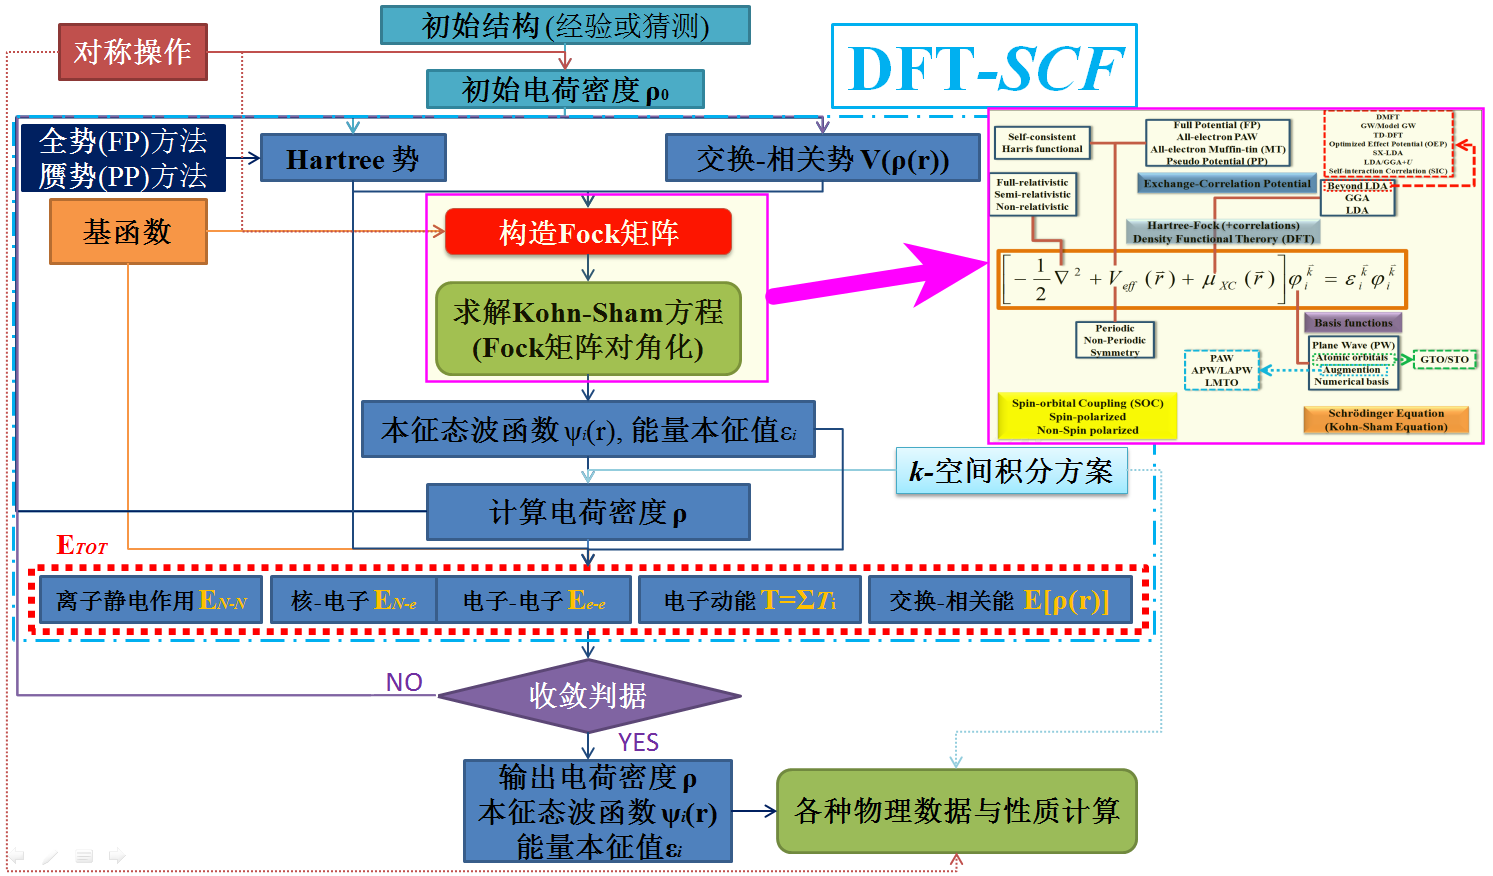
\includegraphics[height=2.80in,width=4.95in,viewport=5 3 1490 870,clip]{Figures/DFT-SCF_2.png}
%\caption{\tiny \textrm{Pseudopotential for metallic sodium, based on the empty core model and screened by the Thomas-Fermi dielectric function.}}%(与文献\cite{EPJB33-47_2003}图1对比)
\label{DFT-SCF-2}
\end{figure}
}

\section{固体能带计算方法}       %Bookmark
\frame
{
%\frametitle{The methods on band structure calculation}
\frametitle{固体能带计算方法}
%\vskip 10pt
%\textrm{The mainly difference of all these methods below: the basis sets and the construction of the potential}
\vskip 10pt
常用的固体能带计算方法
\begin{itemize}%[+-| alert@+>]
%\begin{enumerate}%[+-| alert@+>]
\setlength{\itemsep}{12pt}
%  \item \textrm{Plane wave and the pseudo-potential}
	\item	平面波方法
	\item	正交平面波\textrm{(The orthogonalized plane wave, OPW)}和赝势\textrm{(Pseudo-potential, PP)}方法\upcite{Singh,PRB41-7892_1990,JPCM6-8245_1994}
	\item	缀加平面波\textrm{(Augmented plane wave, APW)}方法
	\item	\textrm{MT}轨道\textrm{(Muffin-tin orbitals, MTO)}方法\upcite{LMTO_Book}
	\item	投影子缀加波\textrm{(Projector Augmented Wave, PAW)}方法\upcite{PRB50-17953_1994,PRB59-1758_1999}
\end{itemize}
\vskip 5pt 各种方法的\textcolor{red}{主要区别}:~\textcolor{blue}{势函数的处理}与\textcolor{blue}{所选基函数类型}不同
}

\subsection{赝势理论}       %Bookmark
%\section{Induction on DFT and solid-state physics}       %Bookmark
\frame
{
%\frametitle{The methods on band structure calculation}
	\frametitle{由\textrm{OPW~}到赝势}
%\vskip 10pt
%\textrm{The mainly difference of all these methods below: the basis sets and the construction of the potential}
\begin{itemize}
%\setlength{\itemsep}{5pt}
	\item 完全平面波基组\\{\fontsize{7.5pt}{5.5pt}\selectfont{少数平面波就可以很好地描述波函数在原子间的行为,近核波函数则需要大量平面波展开}}%。因此完全平面波基组虽然方便,但求体系本征态对角化的矩阵非常巨大,计算变得异常耗时。
	\item 正交平面波(\textrm{Orthogonalized plane wave, OPW})方法\\{\fontsize{7.5pt}{5.5pt}\selectfont{价电子用与芯层波函数正交的平面波展开
		\begin{displaymath}
			\phi_{\textrm{OPW}}^{\vec k+\vec G}(\vec r)=\phi_{\textrm{PW}}^{\vec k+\vec G}(\vec r)-\sum_c\langle\varphi_c|\phi_{\textrm{PW}}^{\vec k+\vec G}\rangle\varphi_c(\vec r)
		\end{displaymath}}}
	{\fontsize{7.5pt}{5.5pt}\selectfont{构造赝波函数
		\begin{displaymath}
			\tilde{\phi}_v(\vec r)=\phi_v(\vec r)+\sum_c\langle\varphi_c|\tilde{\phi}_v\rangle\varphi_c(\vec r)
		\end{displaymath}
	代入\textrm{Schr\"odinger}方程
		$$\hat H|\tilde{\phi}_v\rangle-\sum_c\langle\varphi_c|\tilde{\phi}_v\rangle\hat H|\varphi_c\rangle=\varepsilon_v|\tilde{\phi}_v\rangle-\varepsilon_v\sum_c\langle\varphi_c|\tilde{\phi}_v\rangle|\varphi_c\rangle$$
		可有$$\hat H|\tilde{\phi}_v\rangle+\textcolor{blue}{V^R}|\tilde{\phi}_v\rangle=\textcolor{blue}{\varepsilon_v}|\tilde{\phi}_v\rangle$$
		这里排斥势是$$V^R(\vec r,\vec r^{\prime})=\sum_c(\varepsilon_v-\varepsilon_c)|\varphi_c(\vec r^{\prime})\rangle\langle\varphi_c(\vec r)|$$}}
\end{itemize}
}

\frame
{
	\frametitle{由\textrm{OPW~}到赝势}
	\textrm{Phillips-Kleinman}指出,赝势($V^{e\!f\!f}$)-赝波函数(可用$\phi_{PW}^{\vec k+\vec G}$展开)满足\textrm{Schr\"odinger}方程%\upcite{PR116-287_1959}
	$$\bigg(-\dfrac12\nabla^2+\textcolor{red}{V^{e\!f\!f}}\bigg)|\tilde{\phi}_v\rangle=\textcolor{blue}{\varepsilon_v}|\tilde{\phi}_v\rangle$$
	其中$\textcolor{red}{V^{e\!f\!f}}=V(\vec r)+\textcolor{blue}{V^R}$
	\begin{itemize}
		\item 赝势-赝波函数的本征值$\varepsilon_v$与真实体系的价电子能量本征值等价
		\item 赝势$\textcolor{red}{V^{e\!f\!f}}$比$V(\vec r)$平滑得多,并且$\textcolor{blue}{V^R}$是非局域的排斥势
			\begin{displaymath}
				\begin{aligned}
					\textcolor{blue}{V^R}f(\vec r)=&\sum_c(\varepsilon_v-\varepsilon_c)\varphi_c(\vec r)\int\varphi_c^{\ast}(\vec r^{\prime})f(\vec r^{\prime})\mathrm{d}\vec r^{\prime} \\
					=&\int V^R(\vec r,\vec r^{\prime})f(\vec r^{\prime})\mathrm{d}\vec r^{\prime}
				\end{aligned}
			\end{displaymath}
%			这里$$V^R(\vec r,\vec r^{\prime})=\sum_c(\varepsilon_v-\varepsilon_c)|\varphi_c(\vec r^{\prime})\rangle\langle\varphi_c(\vec r)|$$
	\end{itemize}
}

\frame
{
\frametitle{赝势的评估}
赝势(\textrm{Pseudo Potential, PP})方法是在正交平面波的基础上发展起来的,构造出平缓的势函数代替核的强吸引作用和芯层电子的排斥作用,用平缓的函数取代波函数近核时的震荡。
\begin{itemize}
\setlength{\itemsep}{5pt}
	\item 赝势-平面波方法,只需要少量平面波可展开赝波函数,大大提升了计算效率;但是赝波函数不能很好地反映与电子近核行为有关的性质。
	\item 赝势的构造并不唯一,考核构造赝势的两大指标:~\\“柔软程度”\textrm{(Soft)}与“可移植性”\textrm{(transferability)}
\end{itemize}
\begin{figure}[h!]
\centering
\vspace*{-0.10in}
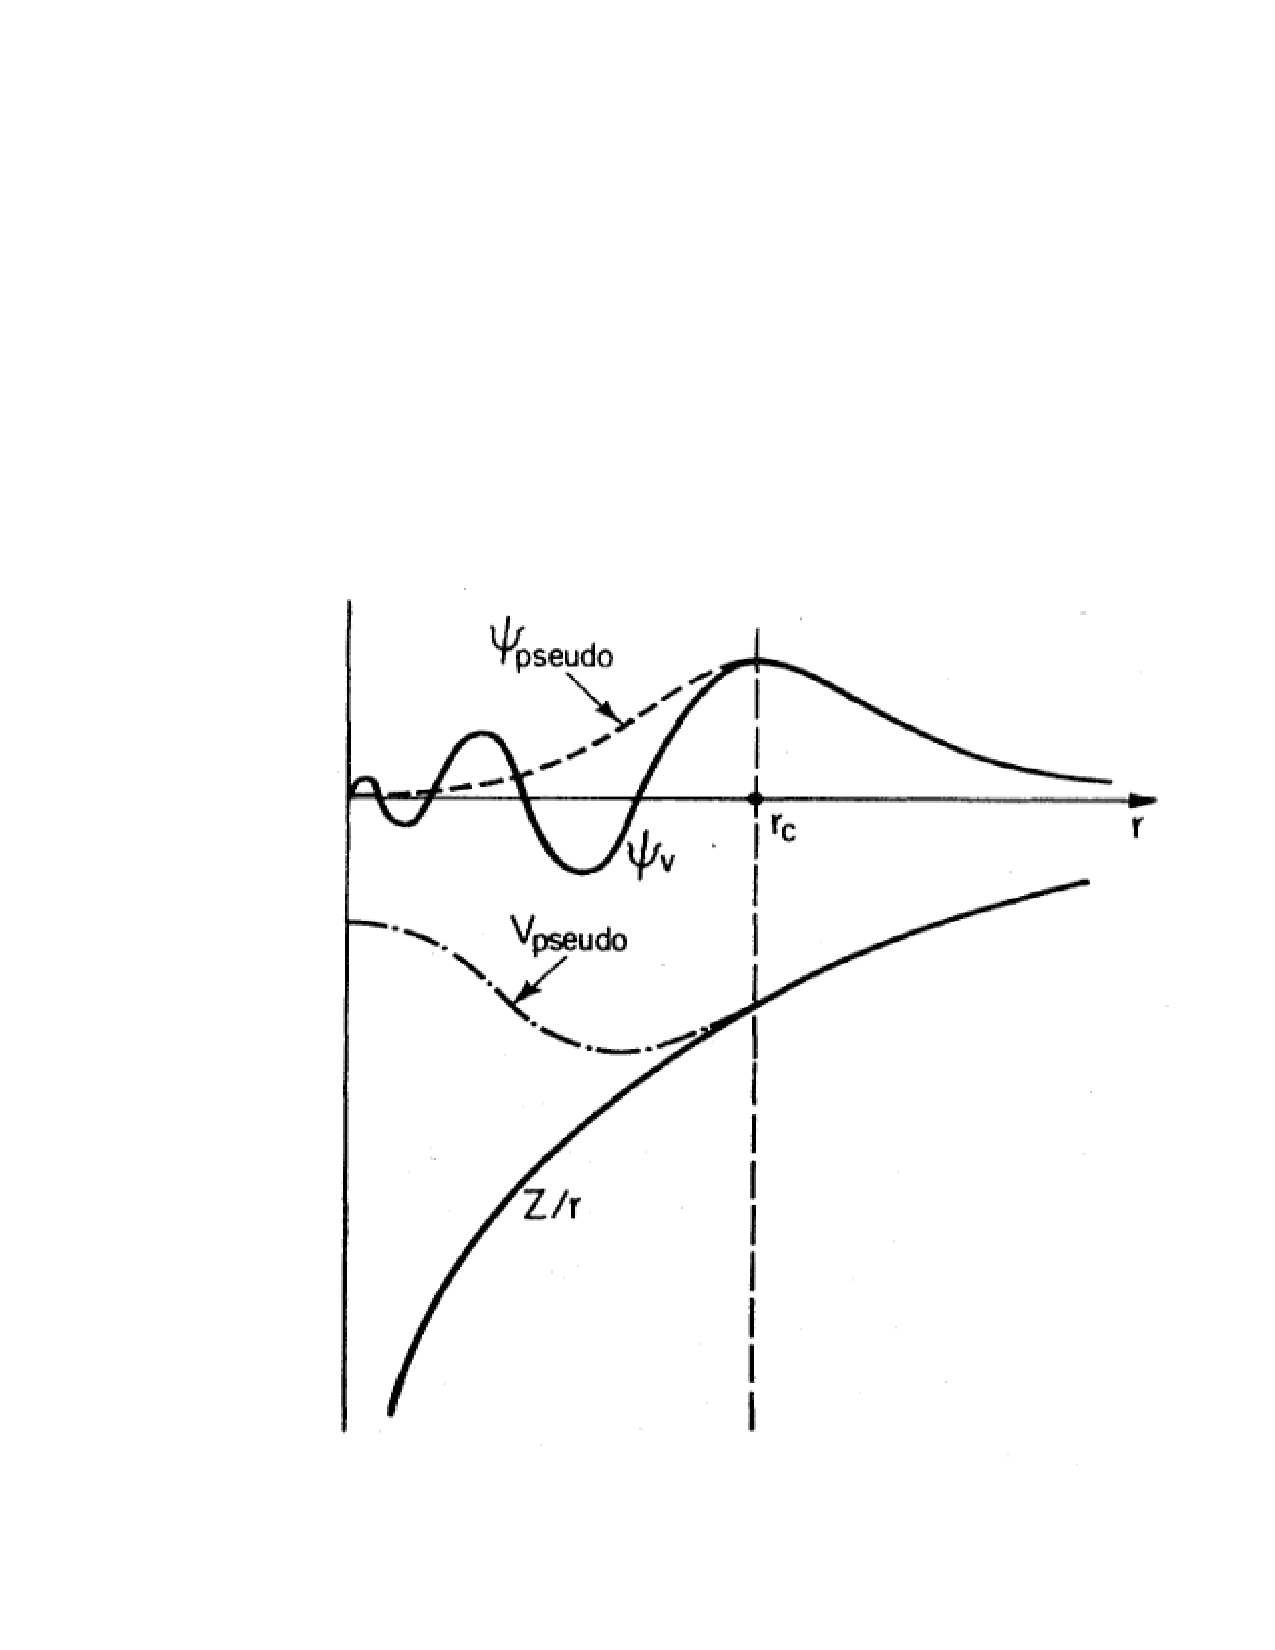
\includegraphics[height=1.35in,width=1.40in,viewport=154 100 562 508,clip]{Figures/Pseudo.pdf}
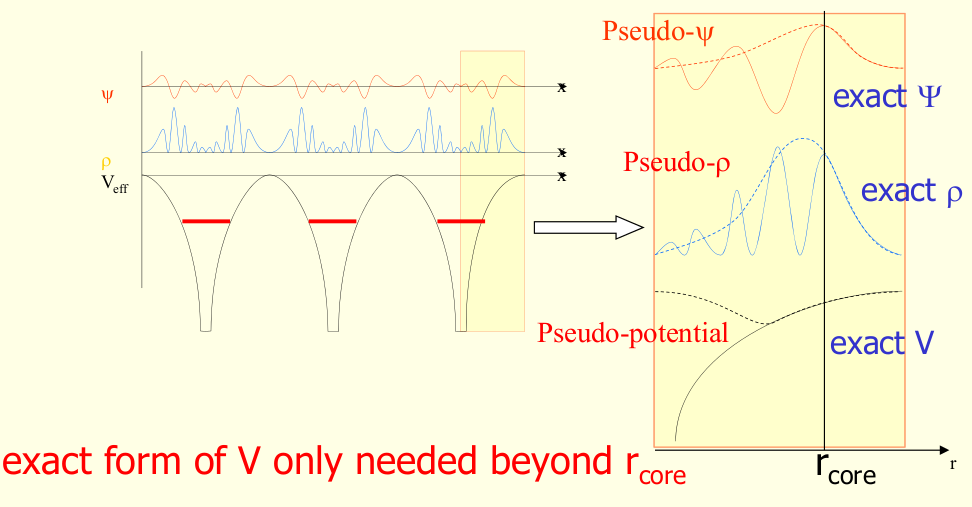
\includegraphics[height=1.35in,width=2.55in,viewport=1 1 980 500,clip]{Figures/Pseudo-2.png}
\caption{\tiny \textrm{The Pseudo wave function and Pseudo potential.}}%(与文献\cite{EPJB33-47_2003}图1对比)
\label{Pseudo_Potential-Wave}
\end{figure}
}

\frame
{
	\frametitle{第一原理赝势}
		由第一原理求解出全电子波函数(径向部分)$P_{n,l}(r)$
			\begin{displaymath}
				\bigg[-\dfrac12\dfrac{\mathrm{d}^2}{\mathrm{d}r^2}+\dfrac{l(l+1)}{2r^2}+V(\rho,r)\bigg]P_{n,l}(r)=\varepsilon_{n,l}P_{n,l}(r)
			\end{displaymath}
			这里$V(\rho,r)$是自洽单电子势
			$$V(\rho,r)=-\frac{Z}r+V_{\mathrm H}(\rho,r)+V_{XC}^{\mathrm{LDA}}(\rho(r))$$
			$V_{\mathrm H}(\rho,r)$是\textrm{Hartree}势,$V_{XC}^{\mathrm{LDA}}(\rho(r))$是交换-相关势

			由此构造赝波函数$P_l^{\mathrm{PP}}(r)$,满足
			$$P_l^{\mathrm{PP}}(r)=P_l^{\mathrm{AE}}(r),\quad r>r_{l}^c$$
			进而构造赝势$V_{\mathrm{src},l}^{\mathrm{PP}}(r)$
			$$V_{\mathrm{src},l}^{\mathrm{PP}}(r)=\varepsilon_l-\dfrac{l(l+2)}{2r^2}+\dfrac{1}{2P_l^{\mathrm{PP}}(r)}\dfrac{\mathrm{d}^2}{\mathrm{d}r^2}P_l^{\mathrm{PP}}(r),\quad r<r_{l}^c$$
}

\frame
{
	\frametitle{模守恒\textrm{(Norm-conserving)}条件}
%	构造赝势确定参数的边界(构造条件)
	\begin{enumerate}
		\item 价电子赝波函数的能量本征值与对应全电子波函数能量本征值相等:~$\varepsilon_l^{\mathrm{PP}}=\varepsilon_l^{\mathrm{AE}}$
		\item 价电子赝波函数与真实电子波函数的径向部分在截断半径$r_{c,l}$外相同:~$\psi_l^{\mathrm{PP}}(r)=\psi_l^{\mathrm{AE}}(r),\quad r>r_{l}^c$
		\item 价电子赝波函数与真实电子波函数的对数导数在截断半径$r_{c,l}$处相等:~$D_l^{\mathrm{PP}}(r)=D_l^{\mathrm{AE}}(r),\quad r\geqslant r_{l}^c$\\
		这里$D_l(\varepsilon,r)=r\frac{\psi_l^{\prime}(\varepsilon,r)}{\psi_l(\varepsilon,r)}=r\dfrac{\mathrm{d}}{\mathrm{d}r}\ln\psi_l(\varepsilon,r)$
		\item 价电子赝波函数与真实电子波函数在截断半径$r_{l}^c$内的积分电荷相等(\textcolor{red}{模守恒条件})
			$$Q_l=\int_0^{r_{l}^c}\mathrm{d}rr^2|\psi_l^{\mathrm{PP}}(r)|^2=\int_0^{r_{l}^c}\mathrm{d}rr^2|\psi_l^{\mathrm{AE}}(r)|^2$$
		\item 价电子赝波函数与真实电子波函数的对数导数一阶能量导数$\mathrm{d}D_l(\varepsilon,r)/\mathrm{d}\varepsilon$在截断半径$r_{l}^c$处及以外相等
	\end{enumerate}
}

\frame
{
	\frametitle{模守恒\textrm{(Norm-conserving)}条件}
\begin{figure}[h!]
\centering
\vspace*{-0.10in}
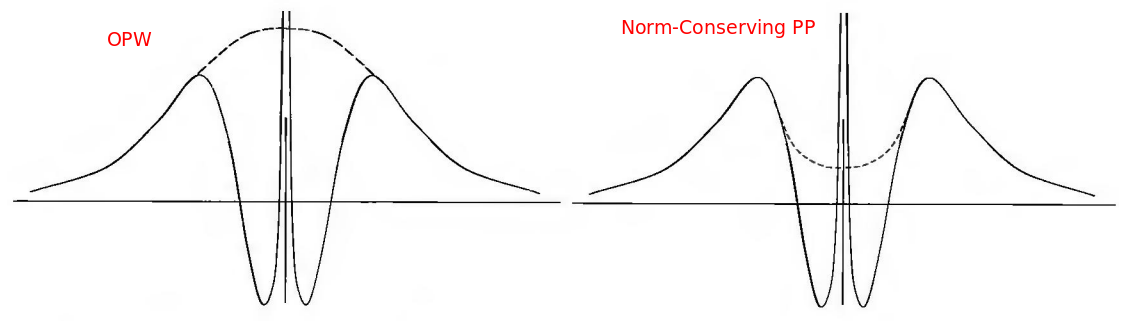
\includegraphics[height=1.30in,width=4.17in,viewport=0 0 1150 350,clip]{Figures/Pseudo-OPW_NCPP.png}
\caption{\tiny \textrm{Schematic example of a valence function that has the character of a $3s$ orbital near the nucleus and two examples of smooth functions (dashed lines) that equal the full wave-function outside the core region. Left: the smooth part of the valence function defined by OPW-like equation; Right: a smooth pseudo-function that satisfies the norm-conservation condition.}}%(与文献\cite{EPJB33-47_2003}图1对比)
\label{Pseudo-OPW_NCPP}
\end{figure}
}

\frame
{
	\frametitle{赝势去屏蔽}
	第一原理赝势建立了赝波函数与对应赝势的一一对应关系,但该赝势包含了电子屏蔽(原子、离子环境)信息,去屏蔽后的赝势对环境依赖更低,“可移植性”更好
	$$V_{\mathrm{ion},l}^{\mathrm{PP}}(r)=V_{\mathrm{src},l}^{\mathrm{PP}}(r)-V_{\mathrm{H},l}^{\mathrm{PP}}(r)-V_{XC,l}^{\mathrm{PP}}(r)$$
	去屏蔽过程中,特别需要注意$V_{XC,l}^{\mathrm{PP}}(r)$的处理
	$$V_{XC,l}^{\mathrm{PP}}(r)=V_{XC}^{\mathrm{PP}}([n_l^{\mathrm{PP}}],r)+\big[V_{XC}^{\mathrm{PP}}([n_l^{\mathrm{PP}}+n^{core}],r)-V_{XC}^{\mathrm{PP}}([n_l^{\mathrm{PP}}],r)\big]$$
}

\frame
{
\frametitle{超软赝势}
\begin{itemize}
\setlength{\itemsep}{5pt}
	\item 赝势构造的模守恒条件
%		\begin{displaymath}
%			\int_0^{r_c}\mathrm{d}\vec r\varphi^{\ast PS}(\vec r)\varphi^{PS}(\vec r)=\int_0^{r_c}\mathrm{d}\vec r\varphi^{\ast}(\vec r)\varphi(\vec r)
%		\end{displaymath}
	很好地解决了赝势可移植性问题,但对$1s$、$2p$、$3d$等轨道,模守恒方案构造的赝势过于“硬”,所需平面波基组依然非常大
	\item 超软\textrm{(Ultra-soft)}赝势,解除模守恒条件,实现对第一、第二周期元素的高效计算
\end{itemize}
\begin{figure}[h!]
\vspace*{-0.10in}
\centering
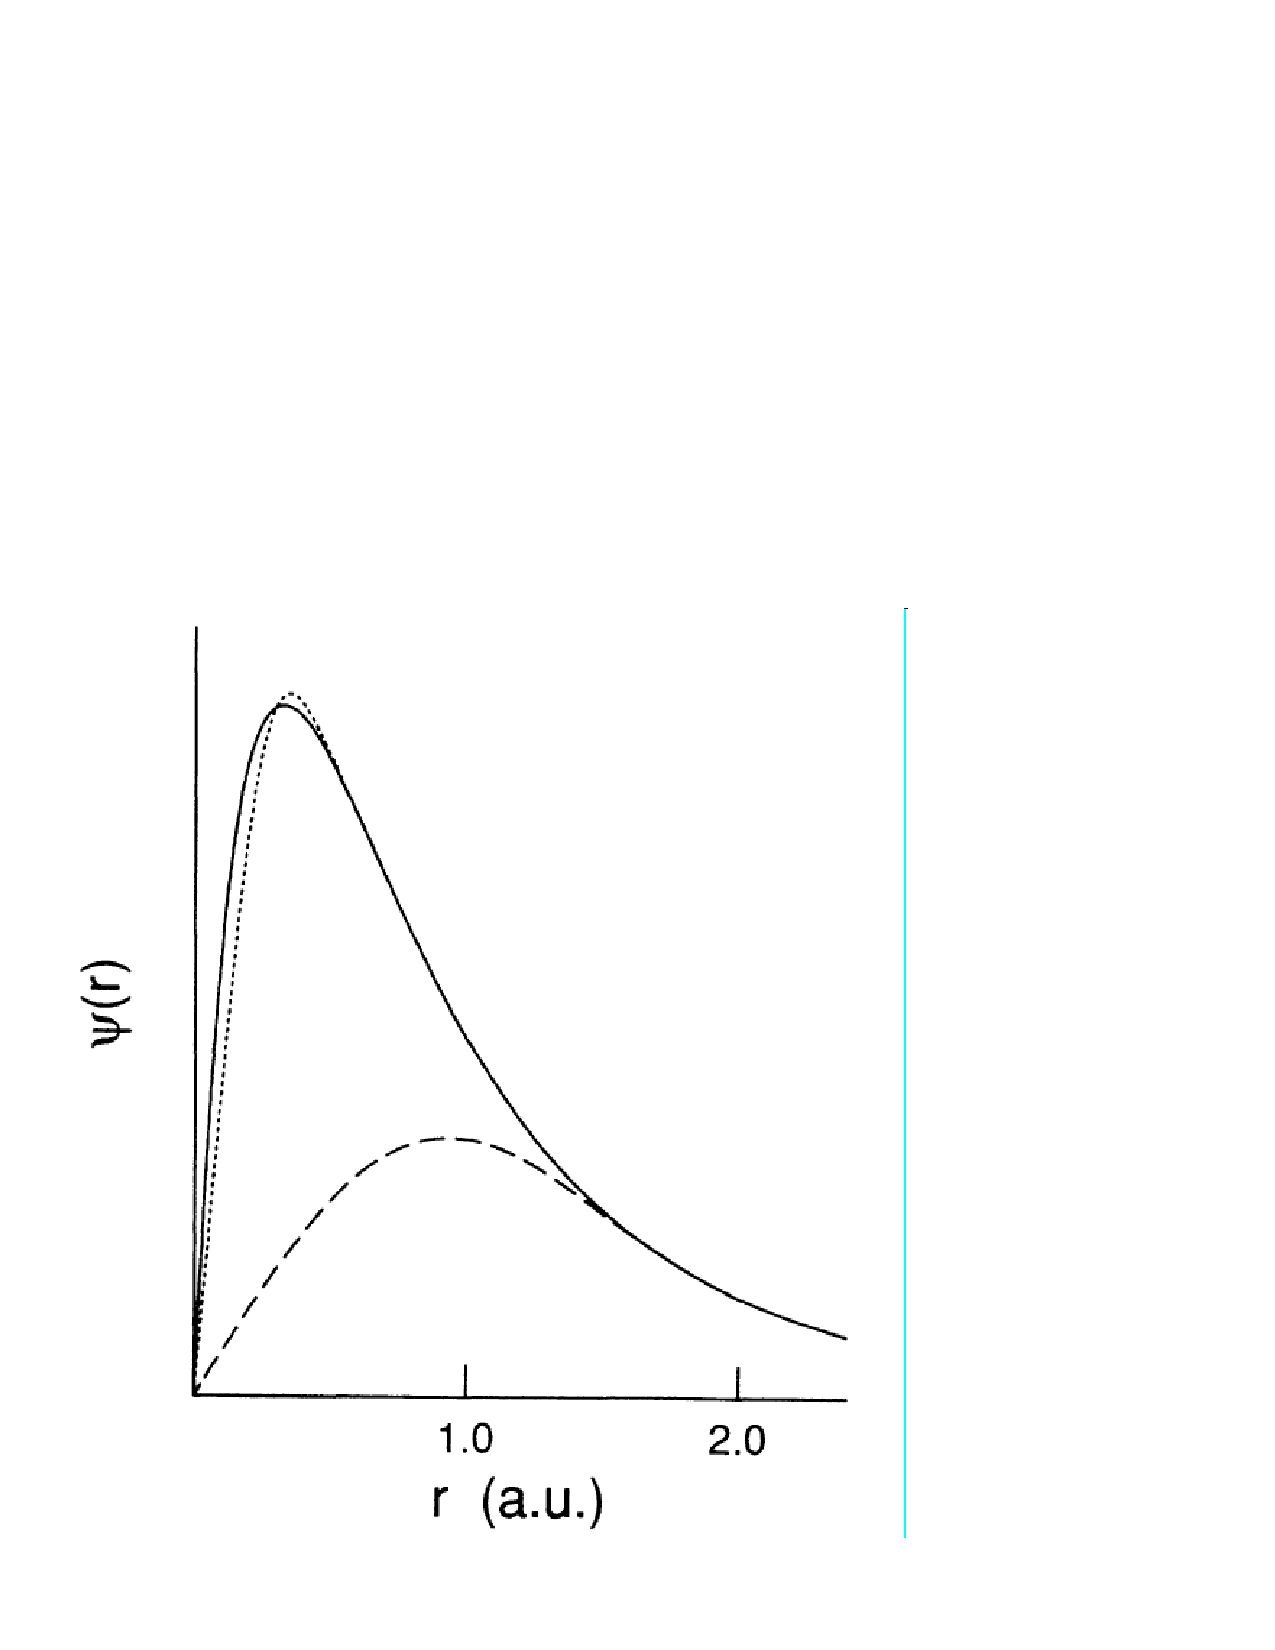
\includegraphics[height=1.35in,width=1.40in,viewport=30 55 415 500,clip]{Figures/Norm-US-wave.pdf}
\caption{\tiny \textrm{Oxygen 2} \textit{p} \textrm{radical wave function (solid), NC-pseudo-wave (dotted) and US-pseudo-wave (dashed).}}%(与文献\cite{EPJB33-47_2003}图1对比)
\label{Norm-US-wave}
\end{figure}
}

\frame
{
\frametitle{补偿电荷与多极矩}
根据电动力学定理:\\\textcolor{blue}{如果球\textrm{S}内的电荷密度分布$\rho(\vec r)$,在球外某点$\vec r$产生的势是由电荷密度的多极矩确定}:
\begin{figure}[h!]
\vspace*{-15pt}
\centering
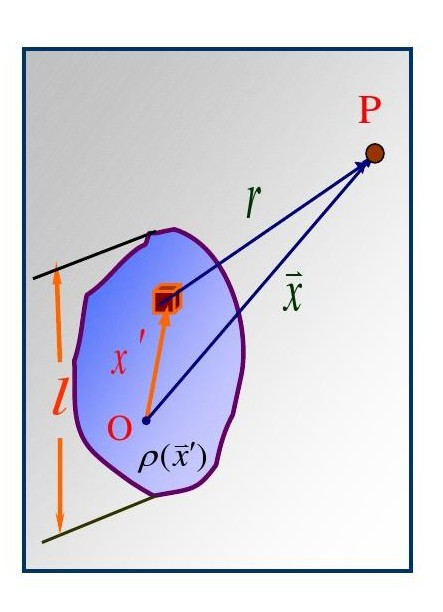
\includegraphics[height=1.25in,width=1.32in,viewport=1 22 507 575,clip]{Figures/potential_multipole.jpg}
%\caption{\tiny \textrm{From Muffin-tin Potential to Full Potential}}%(与文献\cite{EPJB33-47_2003}图1对比)
\label{Potential-multipole}
\end{figure}
\begin{displaymath}
	V(\vec r)=\sum_{l=0}^{\infty}\sum_{m=-l}^{l}\dfrac{4\pi}{2l+1}q_{lm}\dfrac{Y_{lm}(\hat{\vec r})}{r^{l+1}}
\end{displaymath}
其中多极矩$q_{lm}$由下式计算
\begin{displaymath}
	q_{lm}=\int_SY_{lm}^{\ast}(\hat{\vec r})r^l\rho(\vec r)\mathrm{d}^3r
\end{displaymath}
}

\frame
{
\frametitle{超软赝势的构造}
\textrm{Vanderbilt}建议构造赝波函数时放弃模守恒约束条件,只要求价电子赝波函数与真实电子波函数的径向部分在截断半径$r_{l}^c$外相同,由此得到的赝势显然非\textrm{Hermitian},但是通过构造\\\textcolor{blue}{\textrm{Hermitian}重叠算符}
\begin{displaymath}
	\mathbf{S}=\mathbf{1}+\sum_{i,j}Q_{ij}|\beta_j\rangle\langle\beta_i|
\end{displaymath}
以及\textcolor{blue}{\textrm{Hermitian}赝势算符}
\begin{displaymath}
	\tilde V^{\mathrm{NL}}=\sum_{i,j}\mathbf{D}_{i,j}|\beta_j\rangle\langle\beta_i|
\end{displaymath}
这里\textcolor{blue}{
\begin{displaymath}
	\mathbf{D}_{ij}=B_{ij}+\varepsilon_iQ_{ij}
\end{displaymath}}
模守恒约束下的标准本征值方程将变成广义本征值方程
\begin{displaymath}
	(T+V_{\mathrm{loc}}+\tilde V^{\mathrm{NL}}-\varepsilon\mathbf{S})|\phi\rangle=0
\end{displaymath}
}

\frame
{
\frametitle{超软赝势的特点}
\textrm{Vanderbilt}的超软赝势构造方案最大的优点是
\begin{itemize}
	\item \textcolor{purple}{解除模守恒约束}:~有助于增加赝波函数的截断半径,系统提高赝势的柔软程度
	\item \textcolor{purple}{引入多个参考能量$\varepsilon_l$}:~使得模守恒条件下只在特定参考能量$\varepsilon$处成立的对数导数连续条件,扩展到参考能量$\varepsilon_l$区间范围内,这大大提高了赝势的适用范围(可移植性)
\end{itemize}

相应的,超软赝势计算中,电子密度表达形式为
\begin{displaymath}
	n(r)=\sum_nf_n|\phi_n(r)|^2+\sum_{n,ij}f_n\langle\phi_n|\beta_j\rangle\langle\beta_i|\phi_n\rangle Q_{ij}(r)
\end{displaymath}
这里补偿电荷$Q_{ij}(r)$定义为
\begin{displaymath}
	Q_{ij}(r)=\phi_i^{\mathrm{AE}}(r)\phi_j^{\mathrm{AE}}(r)^{\ast}-\phi_i^{\mathrm{US}}(r)\phi_j^{\mathrm{US}}(r)^{\ast}
\end{displaymath}
}

\subsection{\rm{APW~}与\rm{LAPW~}方法}
\frame
{
\frametitle{\textrm{APW}方法}
\begin{figure}[h!]
\centering
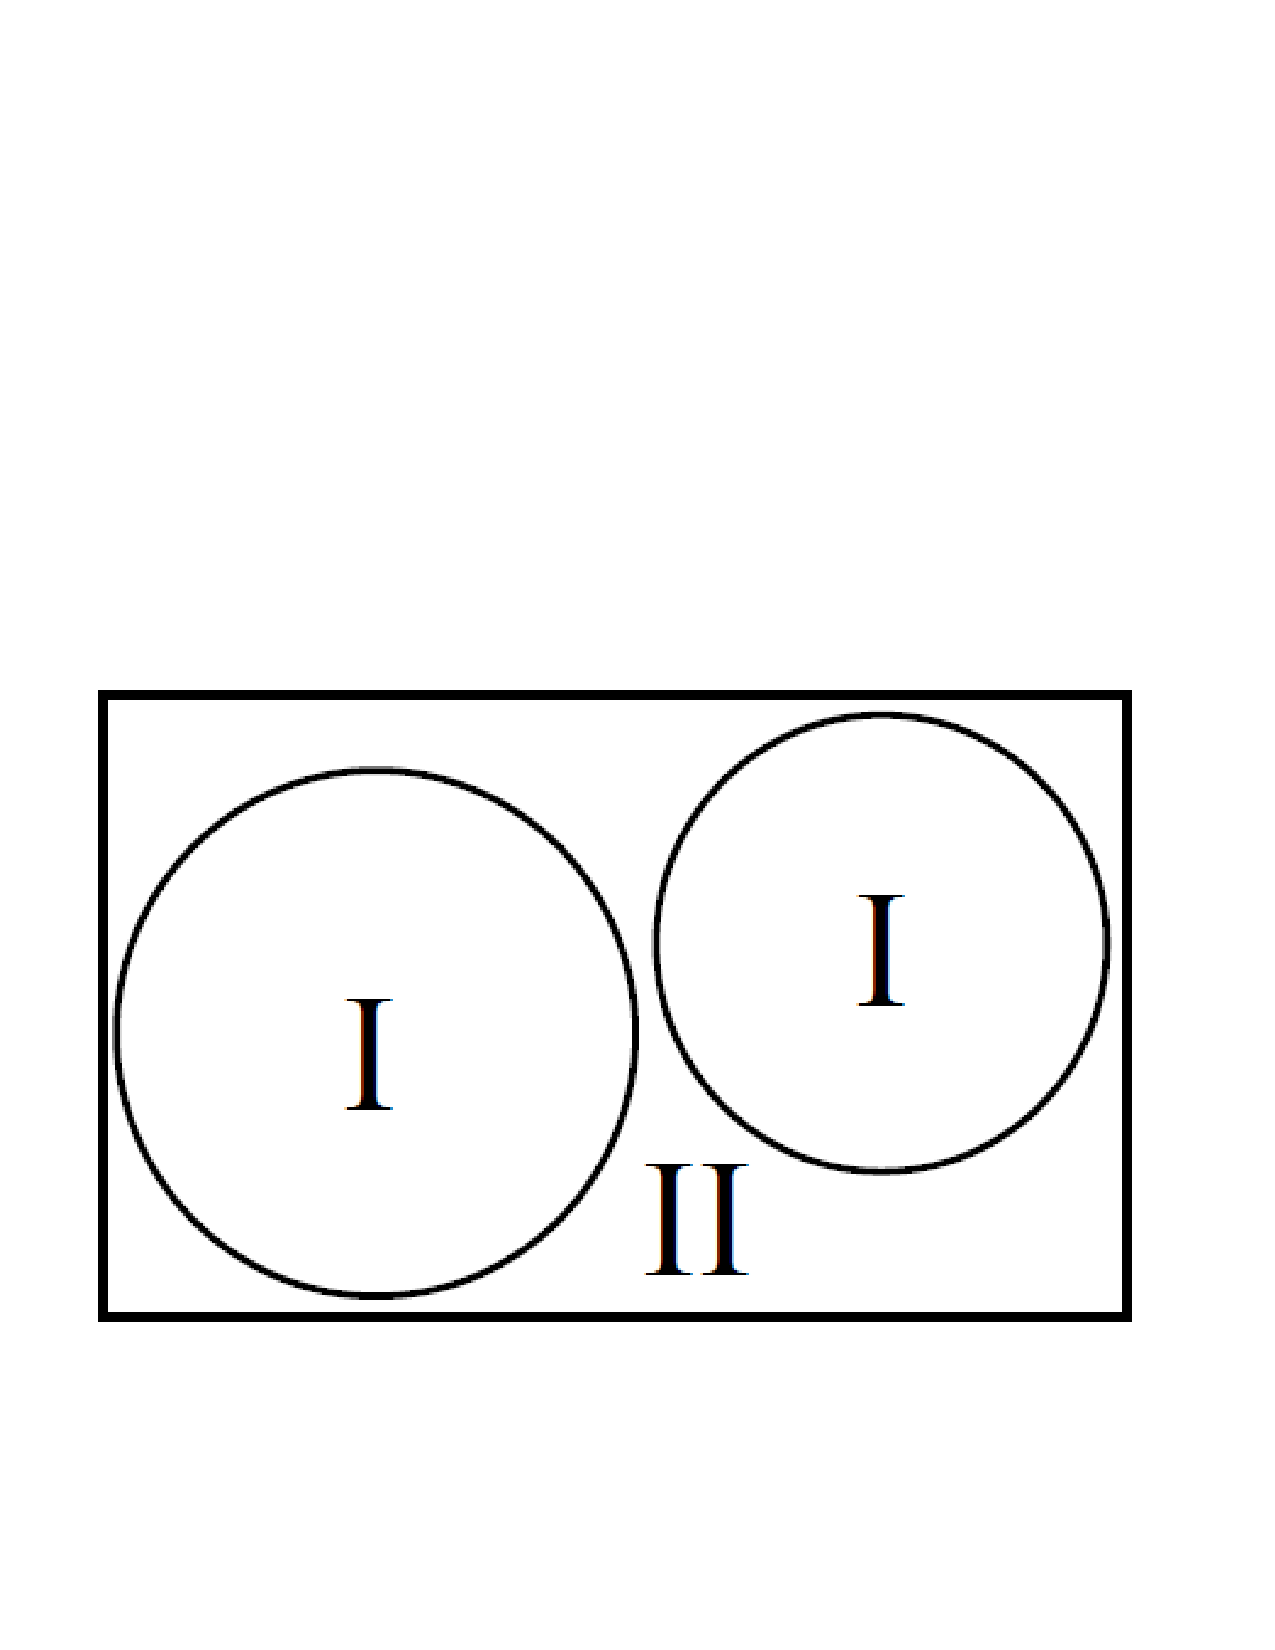
\includegraphics[height=1.10in,width=1.80in,viewport=40 150 545 465,clip]{Figures/Muffin_tin.pdf}
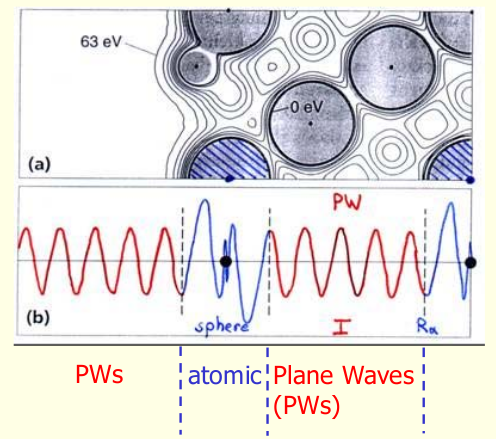
\includegraphics[height=1.10in,width=1.45in,viewport=1 20 485 435,clip]{Figures/APW.png}
\caption{\tiny \textrm{Partitioning of the unit cell into atomic spheres(I) and an interstitial region(II)}}%(与文献\cite{EPJB33-47_2003}图1对比)
\label{Muffin_tin-2}
\end{figure}
\begin{displaymath}
\hskip -28pt\footnotesize \varphi(\vec k_j,\vec r)=\left\{
  \begin{aligned}
    &\Omega^{-1/2}\exp[i\vec k_j\cdot\vec r],&|\vec r-\vec r_s|>R_{\mathrm{MT}}^s\\
    &\sum_{lm}A_{lm}u_l(|\vec r-\vec r_s|,E)Y_{lm}(\widehat{\vec r-\vec r_s}),&|\vec r-\vec r_s|\leqslant R_{\mathrm{MT}}^s
  \end{aligned}
\right.
\end{displaymath}
}

\frame
{
	\frametitle{空间两部分函数在球面上的衔接}
	\textrm{Huygens}原理:~\textcolor{blue}{平面波可以在各个原子球中心用球谐函数展开}:
	\begin{displaymath}
		\mathrm{e}^{\mathrm{i}\vec k\cdot\vec r}=4\pi\sum_{l=0}^{\infty}\sum_{m=-l}^l\mathrm{i}^lj_l(|\vec k|r)Y_{lm}^{\ast}(\hat{\vec k})Y_{lm}(\hat{\vec r})
	\end{displaymath}
	其中$j_l(|\vec k|r)$是$l$-阶球\textrm{Bessel}函数,$\hat{\vec k}$和$\hat{\vec r}$分别是矢量$\vec k$和$\vec r$与直角坐标$z$-轴的夹角$\theta$和$\varphi$

	要求空间中不同区域函数在球面上连续,可调参数$A_{lm}^{\vec k}$可为下式确定
\begin{displaymath}
	A_{lm}^{\vec k}=4\pi\mathrm{e}^{\mathrm{i}\vec k\cdot\vec r_s}\mathrm{i}^lY_{lm}^{\ast}(\hat{\vec k})j_l(|\vec k|R_{MT}^s)/u_l(R_{MT}^s,E)
\end{displaymath}
\textrm{APW}的问题:\textcolor{blue}{球面参数$A_{lm}^{\vec k}$对能量$E$依赖,由此构造的久期方程\footnote{\fontsize{7.2pt}{6.2pt}\selectfont{久期方程\textrm{secular~equation},\textrm{secular}来自拉丁语\textrm{saeculum},本意为一代人、一个时期、一个时代、一个世界等意思。其名词在拉丁语中就作为世纪讲。汉译\textrm{secular}为久期,是取\textrm{long-term}的意思(实为慢,\textrm{slow~in~comparison~to~the~annual~motion}的意思),与期待\textrm{(expectation)}无关。}}非线性的}
}

\frame
{
\frametitle{\textrm{LAPW}方法}
%\small\textrm{APW}方法的困难,久期方程不能化成广义本征值方程的形式(久期方程对能量$E$是非线性的)为了克服这一困难,人们提出线性化方法,
\textrm{O.~K.~Andersen~}提出\textrm{LAPW}方法\upcite{Singh}:将$u_l(r,E)$在某一合适的$E_l$值附近对$E$的一阶微商{$\left.\dfrac{\textrm{d}u_l(r,E)}{\textrm{d}E}\right|_{E_l}\equiv\dot u_l(r,E_l)$}\\代入\textrm{APW}基函数中可得\textrm{LAPW}方法的基函数:
{\fontsize{7.5pt}{3.3pt}\selectfont
$$\hskip -14pt \varphi(\vec k_j,\vec r)=\left\{
  \begin{aligned}
    &\Omega^{-1/2}\exp[i\vec k_j\cdot\vec r],&|\vec r-\vec r_s|>R_{\mathrm{MT}}^s\\
    &\sum_{lm}[A^{\vec k_j}_{lm}u_l(|\vec r-\vec r_s|,E_l)+B^{\vec k_j}_{lm}\dot u_l(|\vec r-\vec r_s|,E_l)]Y_{lm}(\widehat{\vec r-\vec r_s}),&|\vec r-\vec r_s|\leqslant R_{\mathrm{MT}}^s
  \end{aligned}
\right.$$
%$$\Psi_{\vec k}(\vec r)=\int_{\Omega}\tilde G_{\vec k}(\vec r-\vec r\,^\prime;E)V(\vec r\,^\prime)\Psi_{\vec k}(\vec r\,^\prime)\textrm{d}\vec r\,^\prime$$
根据基函数在\textrm{MT}球面上连续到一阶,确定系数$A^{\vec k}_{lm}$,$B^{\vec k}_{lm}$的值。}
\begin{figure}[h!]
	\vskip -3pt
\centering
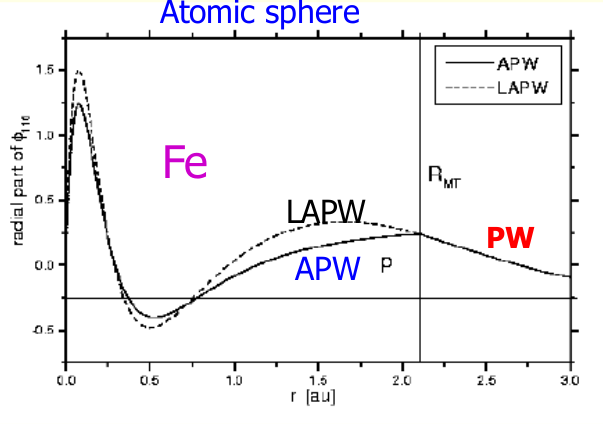
\includegraphics[height=1.10in,width=1.88in,viewport=1 20 585 435,clip]{Figures/WIEN2k-LAPW.png}
\caption{\tiny \textrm{Partitioning of the unit cell into atomic spheres(I) and an interstitial region(II)}}%(与文献\cite{EPJB33-47_2003}图1对比)
\label{Muffin_tin-3}
\end{figure}
}

\subsection{\rm{MTO~}与\rm{LMTO~}方法}
\frame
{
\frametitle{\textrm{MTO}方法}
\textrm{MTO (Muffin-tin Orbial)}方法是\textrm{Andersen}于\textrm{1971}年提出的局域缀加基函数方案\upcite{Andersen_Book}
%\textrm{MTO}的
\vskip 5pt
\textcolor{blue}{目的:~用最小基组方法解析电子结构}
\begin{itemize}
	\item \textcolor{red}{物理图像}:~和\textrm{APW}方法类似,要求基函数在\textrm{MT}球内、外分区域表示,并且在球面上连续
	\item \textcolor{red}{数学形式}:~基函数是最小优化基组
\end{itemize}
\begin{figure}[h!]
	\vspace{-5pt}
\centering
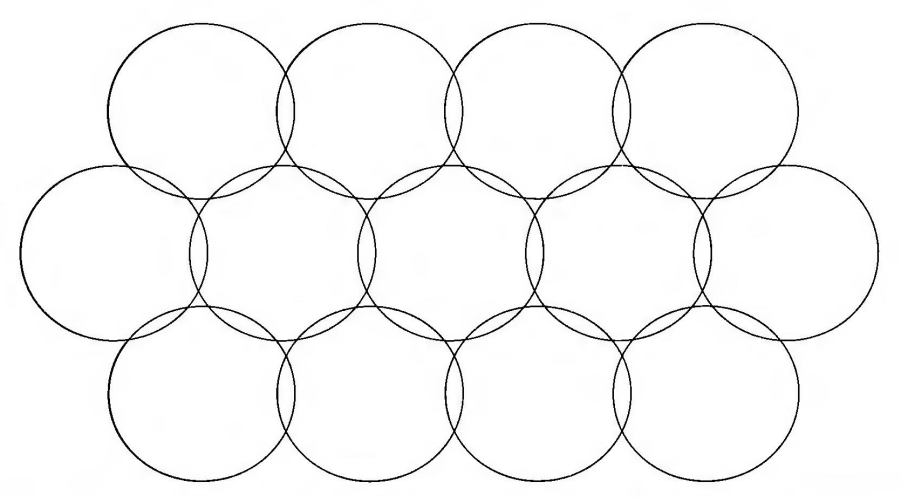
\includegraphics[height=1.20in,width=2.42in,viewport=5 0 1005 495,clip]{Figures/Atomic_sphere-appro.png}
\caption{\fontsize{6.2pt}{4.2pt}\selectfont\textrm{Atomic sphere approximation (ASA) in which the MT spheres are chosen to have the same volume as the Wigner-Seitz cell, which leads to overlapping spheres.}}
\label{Atomic_sphere-appro}
\end{figure}
}

\frame
{
	\frametitle{\textrm{MTO}方法的基函数}
\begin{figure}[h!]
	\vspace{-13pt}
\centering
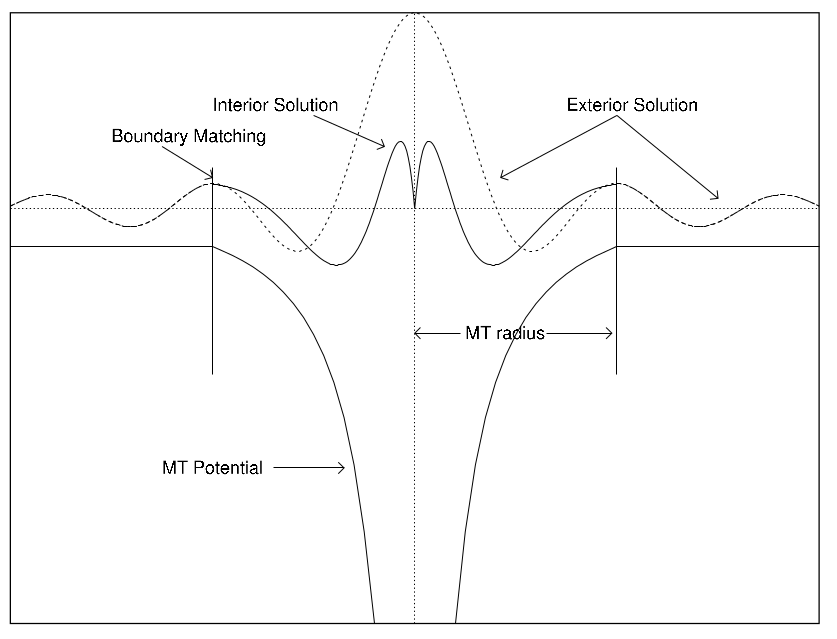
\includegraphics[height=1.25in,width=1.95in,viewport=0 0 845 635,clip]{Figures/MTO-envelope-1.png}
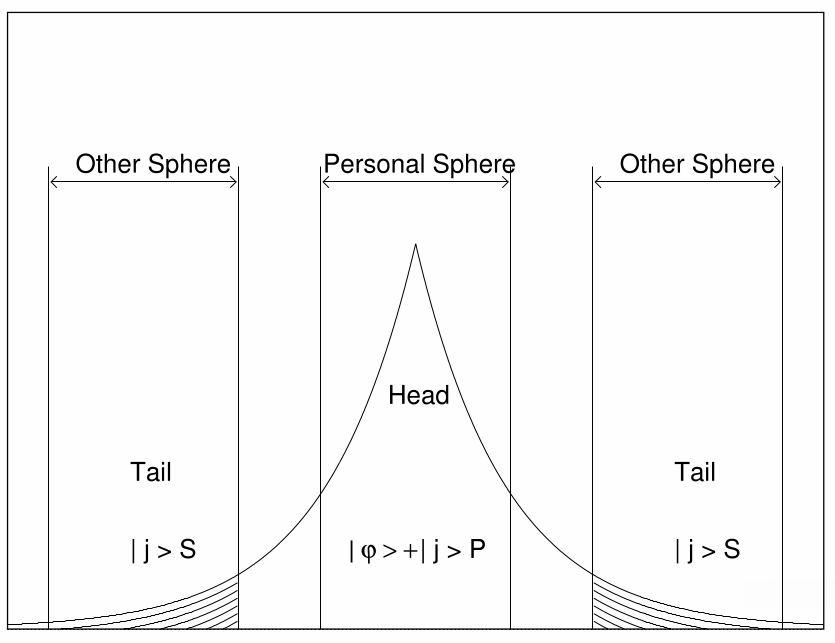
\includegraphics[height=1.25in,width=1.95in,viewport=0 0 885 635,clip]{Figures/MTO-envelope-2.png}
\caption{\tiny \textrm{The radial function of MTO expressed in different region.}}%(与文献\cite{EPJB33-47_2003}图1对比)
\label{MTO-envelope}
\end{figure}
当$q_0=0$时,构成最简单的\textrm{MTO}基函数
		\begin{displaymath}
			\hspace*{-12pt}\chi_L^{\mathrm{MTO}}(\varepsilon,0,\vec r)=\mathrm{i}^lY_L(\hat{\vec r})u_l(\varepsilon,S)\left\{
			\begin{aligned}
				&\dfrac{u_l(\varepsilon,r)}{u_l(\varepsilon,S)}-\dfrac{D_l(\varepsilon)+l+1}{2l+l}\left(\dfrac rS\right)^l&\, r\leqslant S\\
				&+\dfrac{l-D_l(\varepsilon)}{2l+1}\left(\dfrac Sr\right)^{l+1}&\, r>S
			\end{aligned}\right.
		\end{displaymath}
}

\frame
{
	\frametitle{\textrm{MTO}轨道的“尾部抵消”}
\begin{figure}[h!]
	\vspace*{-0.7in}
\centering
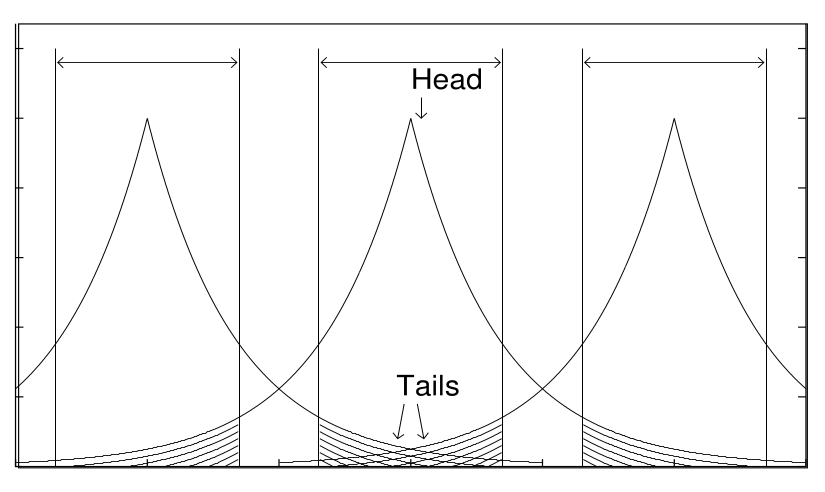
\includegraphics[height=2.55in,width=3.15in,viewport=0 0 845 635,clip]{Figures/MTO-Tail_cancellation.png}
\caption{\tiny \textrm{The wavefunction in the spere at the origin is the sum of the ``head function'' in that sphere plus the tails from neighboring spheres. The schematic illustration of the ``tail cancellation'' of the MTO.}}%(与文献\cite{EPJB33-47_2003}图1对比)
\label{MTO-tail-candellation}
\end{figure}
}

\frame
{
	\frametitle{\textrm{LMTO}方法}
	与\textrm{LAPW}方法类似,在给定能量$\varepsilon_v$和衰减常数$q_0$附近,\textrm{LMTO}的基函数球内部分用函数$\psi_l(\varepsilon_v,r)$及其对能量导数$\dot\psi(\varepsilon_v,r)$表示\\
\textcolor{blue}{\textrm{LMTO}与\textrm{MTO}基函数的区别}
	\begin{itemize}
		\item 球内部分的$\psi(\varepsilon,r)$是主要部分:~由$\psi(\varepsilon_v,r)$和$\dot\psi(\varepsilon_v,r)$线性组合
		\item 球内来自其它\textrm{MT}球的函数尾部贡献被$\dot\psi(\varepsilon_v,r)$的线性组合替代
	\end{itemize}
	由此根据物理直觉,可以把\textrm{LMTO}基函数的形式表示成
		\begin{displaymath}
			\hspace*{-12pt}\chi_L^{\mathrm{LMTO}}(\varepsilon,q_0,\vec r)=\mathrm{i}^lY_L(\hat{\vec r})\left\{
			\begin{aligned}
				&u_l(\varepsilon,r)-q_0\cot(\eta_l(\varepsilon))J_l(q_0r)&\, r\leqslant S\\
				&q_0N_l(q_0r)&\, r>S
			\end{aligned}\right.
		\end{displaymath}
		实际应用中,选定函数$J_l$和$N_l$与球\textrm{Bessel}函数$j_l$和\textrm{Neumann}函数$n_l$相似
}

\frame
{
	\frametitle{\textrm{LMTO~.vs.~LAPW}}
\begin{figure}[h!]
\centering
\vspace*{-0.15in}
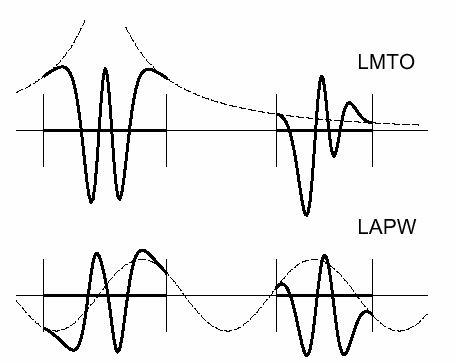
\includegraphics[height=2.50in,width=3.30in,viewport=0 0 440 350,clip]{Figures/LMTO-vs-LAPW.png}
\caption{\fontsize{5.5pt}{4.2pt}\selectfont{\textrm{Schematic illustration of LMTO vs LAPW.}}}%(与文献\cite{EPJB33-47_2003}图1对比)
\label{LMTO-vs-LAPW}
\end{figure}
}

\subsection{\rm{PAW}方法}
\frame
{
	\frametitle{\textrm{PAW}方法概要}
\begin{itemize}
	\item 与芯层态正交的全部价电子构成的\textrm{Hilbert}空间%,价电子彼此的正交使得波函数在\textrm{Muffin-tin}球内振荡
	\item 作\textcolor{red}{线性空间变换},全电子波函数$|\Psi\rangle$与赝波函数$|\tilde\Psi\rangle$满足:
		$$|\Psi\rangle=\mathbf{\tau|}\tilde\Psi\rangle$$
%	$$\tau=\mathbf{1}+\sum_{\mathrm R}\hat\tau_{\mathrm R}$$
	\item 在原子核附近的$r_c$范围内,波函数用原子分波函数展开:
	$$|\Psi\rangle=|\tilde\Psi\rangle+\sum_i(|\phi_i\rangle-|\tilde\phi_i\rangle)\langle\tilde p_i|\tilde\Psi\rangle$$
	\item 在$r_c$外$|\tilde\Psi\rangle$与$|\Psi\rangle$变换前后保持不变,因此线性变换$\mathbf{\tau}$可表示为:
	$$\mathbf{\tau}=\mathbf{1}+\sum_i(|\phi_i\rangle-|\tilde\phi_i\rangle)\langle\tilde p_i|$$
\end{itemize}
其中$|\tilde p_i\rangle$是\textrm{MT}球内的投影函数\\
$i$表示原子位置$\vec R$、原子轨道($l,m$)和能级$\epsilon_k$的指标。
}

\frame
{
%	\frametitle{\textrm{PAW}原子数据集}
	\frametitle{\textrm{PAW}方法的基本思想}
\begin{figure}[h!]
\centering
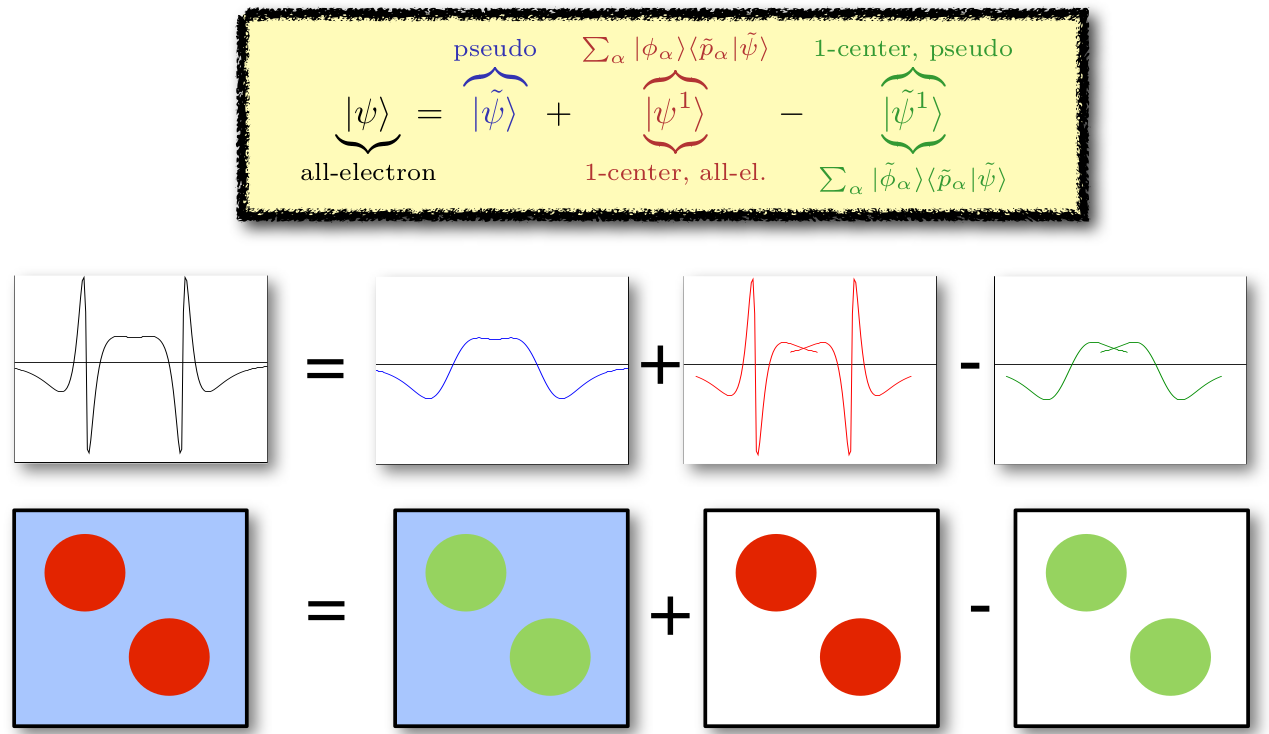
\includegraphics[height=2.3in,width=4.0in,viewport=0 0 1280 745,clip]{Figures/PAW-baseset.png}
\caption{\tiny \textrm{The Augmentation of PAW.}}%(与文献\cite{EPJB33-47_2003}图1对比)
\label{PAW_baseset}
\end{figure}
}

\frame
{
\frametitle{\textrm{PAW}方法的基本思想}
	在赝波函数$|\tilde\Psi\rangle$表象下,算符期望值计算满足$$\langle A \rangle=\langle\Psi|\mathbf{A}|\Psi\rangle=\langle\tilde\Psi|\mathbf{\tau}^{\dag}\mathbf{A}\mathbf{\tau}|\tilde\Psi\rangle=\langle\tilde\Psi|\tilde{\mathrm{A}}|\tilde\Psi\rangle$$
\begin{itemize}
	\item 一般赝算符$\tilde A$表示为
		$$\tilde A=\mathbf{A}+\sum_i|\tilde p_i\rangle(\langle\phi_i|\mathbf{A}|\phi_i\rangle-\langle\tilde\phi_i|\mathbf{A}|\tilde\phi_i\rangle)\langle\tilde p_i|$$
	\item 赝重叠算符$\tilde O$表示为
		$$\tilde O=\mathbf{1}+\sum_i|\tilde p_i\rangle(\langle\phi_i|\phi_i\rangle-\langle\tilde\phi_i|\tilde\phi_i\rangle)\langle\tilde p_i|$$
\end{itemize}
}

\frame
{
\frametitle{\textrm{PAW}方法密度计算}
在\textrm{PAW}框架下,将密度算符$|\vec r\rangle\langle\vec r|$代入,可知密度表达式为
$$n(\vec r)=\tilde n(\vec r)+n^1(\vec r)-\tilde n^1(\vec r)$$
这里
$$\tilde n(\vec r)=\sum_nf_n\langle\tilde\Psi_n|\vec r\rangle\langle\vec r|\tilde\Psi_n\rangle$$ 
$$n^1(\vec r)=\sum_{n,(i,j)}f_n\langle\tilde\Psi_n|\tilde p_i\rangle\langle\phi_i|\vec r\rangle\langle\vec r|\phi_j\rangle\langle\tilde p_j|\tilde\Psi_n\rangle$$
$$\tilde n^1(\vec r)=\sum_{n,(i,j)}f_n\langle\tilde\Psi_n|\tilde p_i\rangle\langle\tilde\phi_i|\vec r\rangle\langle\vec r|\tilde\phi_j\rangle\langle\tilde p_j|\tilde\Psi_n\rangle$$
}

%\frame
%{
%	\frametitle{\textrm{PAW Augmentation}}
%\begin{figure}[h!]
%\centering
%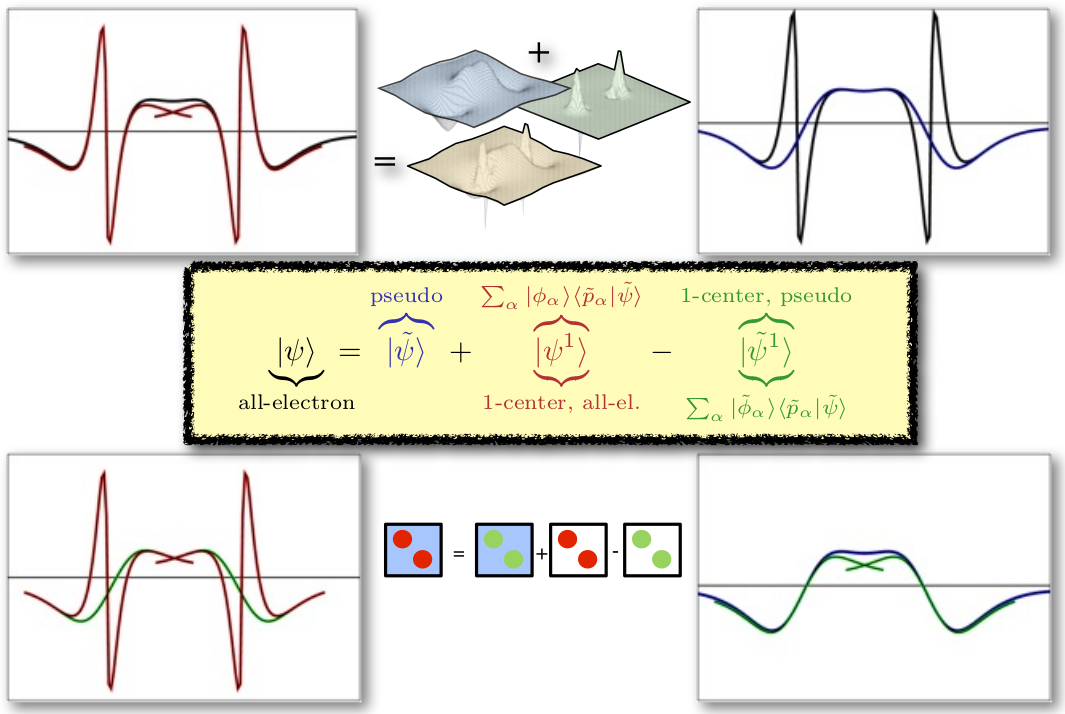
\includegraphics[height=2.3in,width=4.0in,viewport=0 0 1100 745,clip]{Figures/PAW-projector.png}
%\caption{\tiny \textrm{The projector of PAW.}}%(与文献\cite{EPJB33-47_2003}图1对比)
%\label{PAW_projector}
%\end{figure}
%}

\frame
{
\frametitle{电荷密度的重新分解}
\textrm{PAW}方法提出后有很长一段时间没有能够得到广泛应用,直到\textrm{G. Kresse}等将\textrm{Bl\"ochl}的原始方案中电荷密度计算方案重新组合后,明确了\textrm{PAW}方法与\textrm{USPP}方法的内在联系。
\begin{itemize}
	\item 芯层电荷与核电荷构成离子实电荷:$n_{Zc}=n_Z+n_c$
\end{itemize}
\begin{figure}[h!]
\centering
\vspace{-10.5pt}
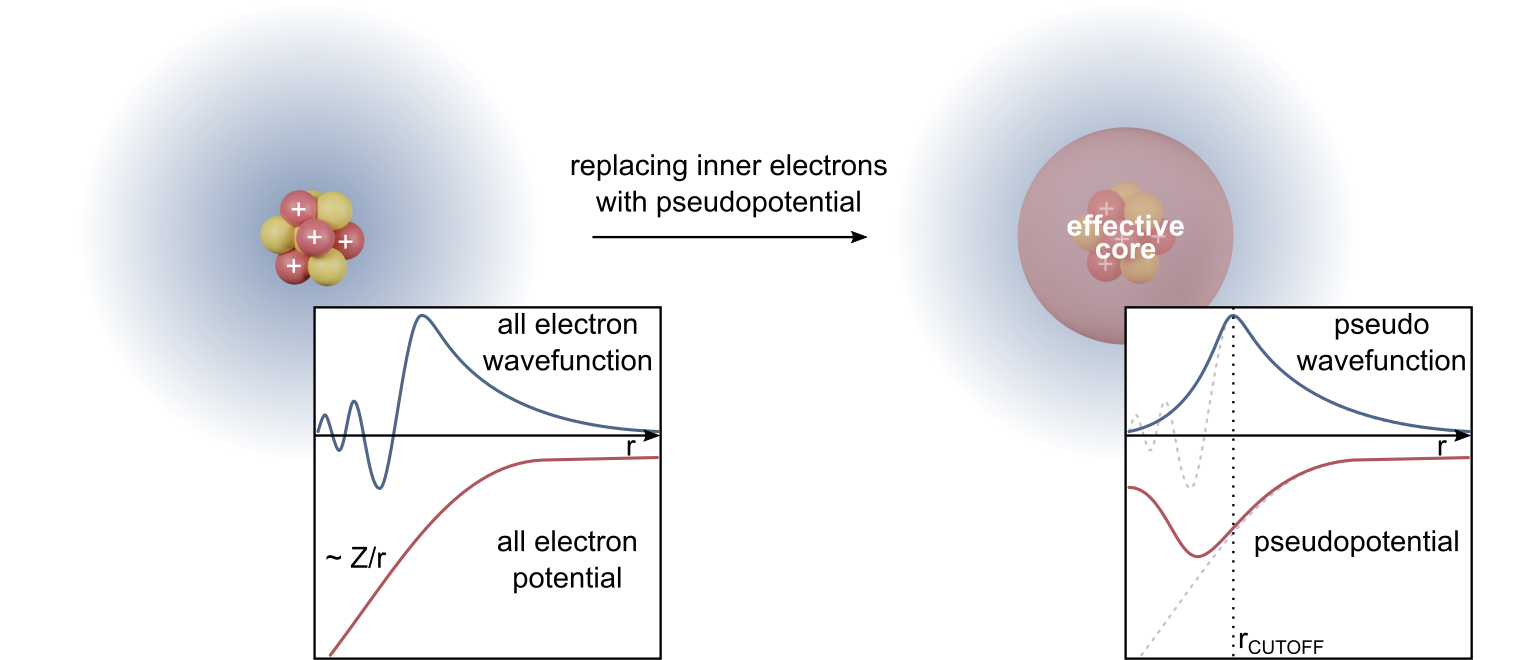
\includegraphics[height=1.5in,width=3.0in,viewport=0 0 380 190,clip]{Figures/Pseudo-potential_charge.png}
\caption{\tiny \textrm{The difference of the electron-density distributing from P.~Bl\"ochl  and from G.~Kresse.}}%(与文献\cite{EPJB33-47_2003}图1对比)
\label{PAW_Pseudo-Charge}
\end{figure}
}

\frame
{
	\frametitle{固体计算方法总结}
\begin{figure}[h!]
\centering
\vspace*{-0.25in}
%\hspace*{-0.80in}
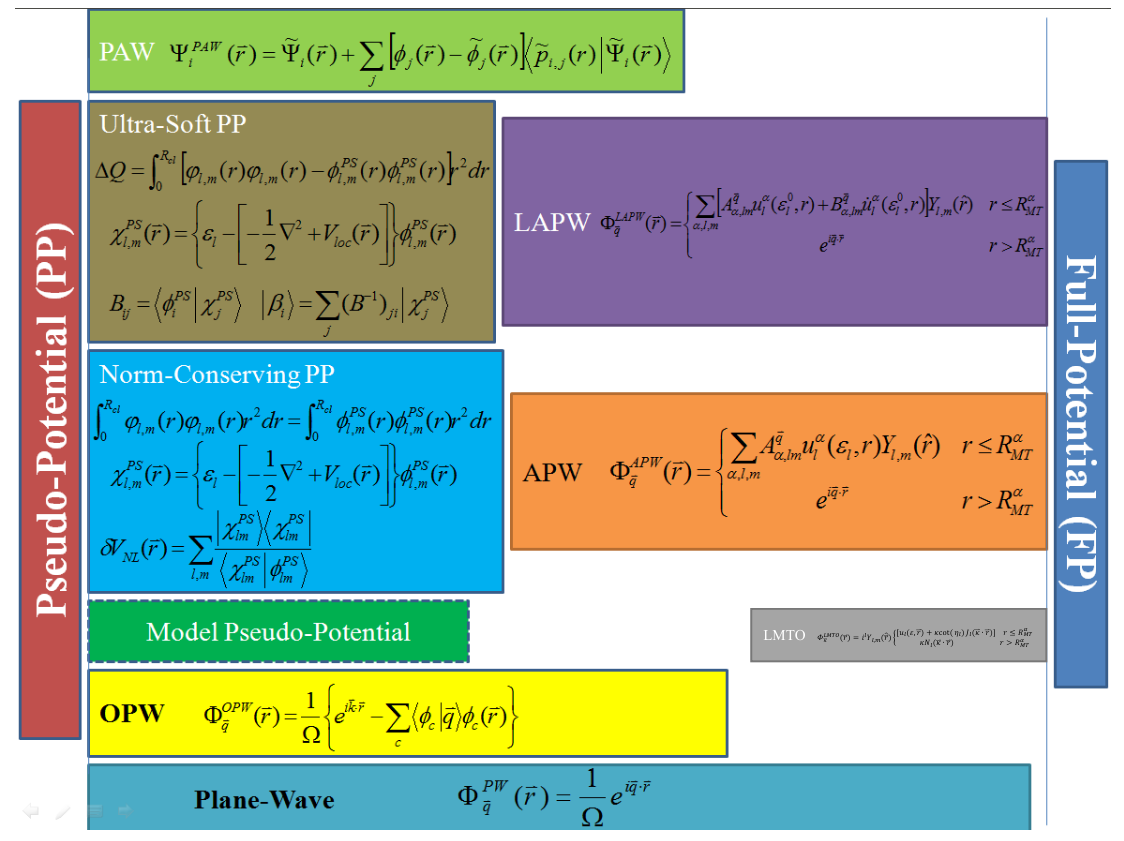
\includegraphics[height=2.80in,width=4.10in,viewport=0 0 1150 850,clip]{Figures/Pseudo-Full_Potential-2.png}
%\caption{\tiny \textrm{Pseudopotential for metallic sodium, based on the empty core model and screened by the Thomas-Fermi dielectric function.}}%(与文献\cite{EPJB33-47_2003}图1对比)
\label{Pseudo-Full_Poential}
\end{figure}
}

		\frame[allowframebreaks]
{
\frametitle{主要参考文献}
\begin{thebibliography}{99}
{\tiny
        \bibitem{Singh}\textrm{D. J. Singh. \textit{Plane Wave, PseudoPotential and the LAPW method} (Kluwer Academic, Boston,USA, 1994)}					%
	\bibitem{PRB41-7892_1990}\textrm{D. Vanderbilt. \textit{Phys. Rev.} B, \textbf{41} (1990), 7892} 
	\bibitem{JPCM6-8245_1994}\textrm{G. Kresse and J. Hafner. J. Phys: \textit{Condens. Matter}, \textbf{6} (1994), 8245}
	\bibitem{LMTO_Book}\textrm{H. Skriver. \textit{The LMTO method} (Springer, New York, USA, 1984)}
	\bibitem{PRB50-17953_1994}\textrm{P. E. Bl\"ochl. \textit{Phys. Rev.} B, \textbf{50} (1994), 17953}
	\bibitem{PRB59-1758_1999}\textrm{G. Kresse and D. Joubert \textit{Phys. Rev.} B, \textbf{59} (1999), 1758}
	\bibitem{Andersen_Book}\textrm{O. K. Andersen. \textit{Computational Methods in Band Theory} (Plenum, New York, USA, 1971)}
	\bibitem{Nemoshkalenko-Antonov}\textrm{V. V. Nemoshkalenko and V. N. Antonov. \textit{Computational Methods in Solid State Physics} (Gordon and Breach Science Publisher, Amsterdam, The Netherlands, 1998)}
	\bibitem{Xie-Lu}谢希德、陆栋\:主编, {\textit{固体能带理论}}\:复旦大学出版社, 上海, 1998
	\bibitem{Elect_Stru}\textrm{Richard. M. Martin. \textit{Electronic Structure: Basic Theory and Practical Methods} (Cambridge University Press, Cambridge, England, 2004)}
	\bibitem{Comp_Phys}\textrm{J. M. Thijssen. \textit{Computational Physics}~\textrm{(2nd Edition)} (Cambridge University Press, Cambridge, England, 2007)}
}
\end{thebibliography}
%\nocite*{}
}

\frame
{
	\frametitle{固体计算软件概览}
\begin{figure}[h!]
\centering
\vspace*{-0.05in}
%\hspace*{-0.80in}
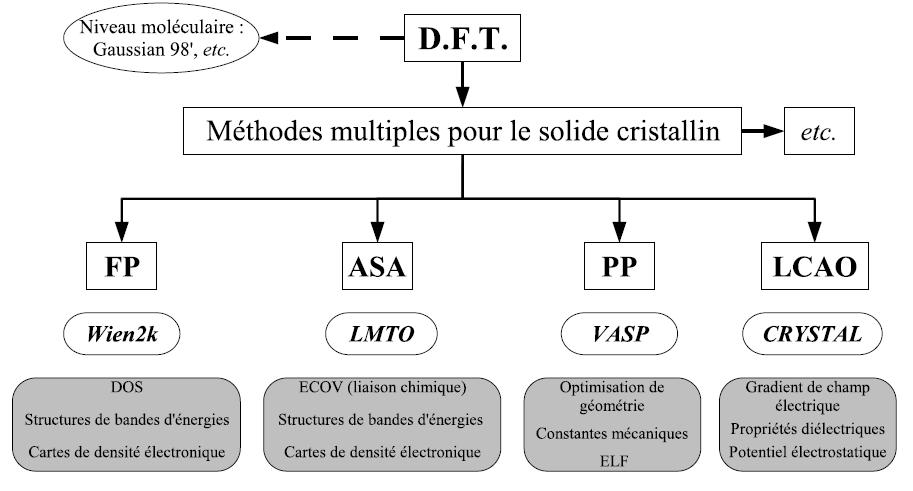
\includegraphics[height=2.30in,width=4.00in,viewport=0 0 920 500,clip]{Figures/DFT-Software.jpg}
%\caption{\tiny \textrm{Pseudopotential for metallic sodium, based on the empty core model and screened by the Thomas-Fermi dielectric function.}}%(与文献\cite{EPJB33-47_2003}图1对比)
\label{Abinitio-Softwares}
\end{figure}
}

\section{计算示例:~\rm{Materials~Studio}建模}
\frame
{
	\frametitle{\textrm{MS}的架构}
\begin{figure}[h!]
\centering
\vspace*{-0.10in}
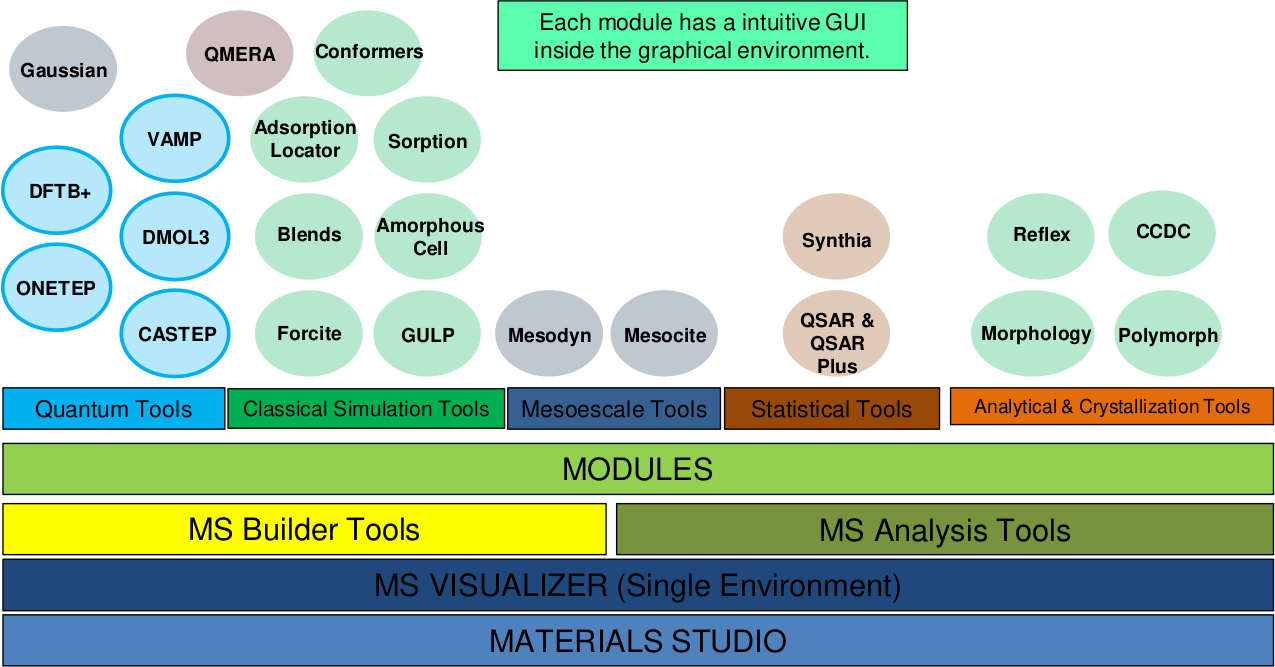
\includegraphics[height=2.20in,width=4.15in,viewport=0 0 1275 667,clip]{Figures/MS-main_Struct.png}
\caption{\tiny \textrm{The main structure of Materials studio.}}%(与文献\cite{EPJB33-47_2003}图1对比)
\label{MS-main-structure}
\end{figure}
}

\subsection{\rm{Materials Studio}的界面框架}
\frame
{
	\frametitle{\textrm{MS}的界面框架}
\begin{figure}[h!]
\centering
\vspace*{-0.31in}
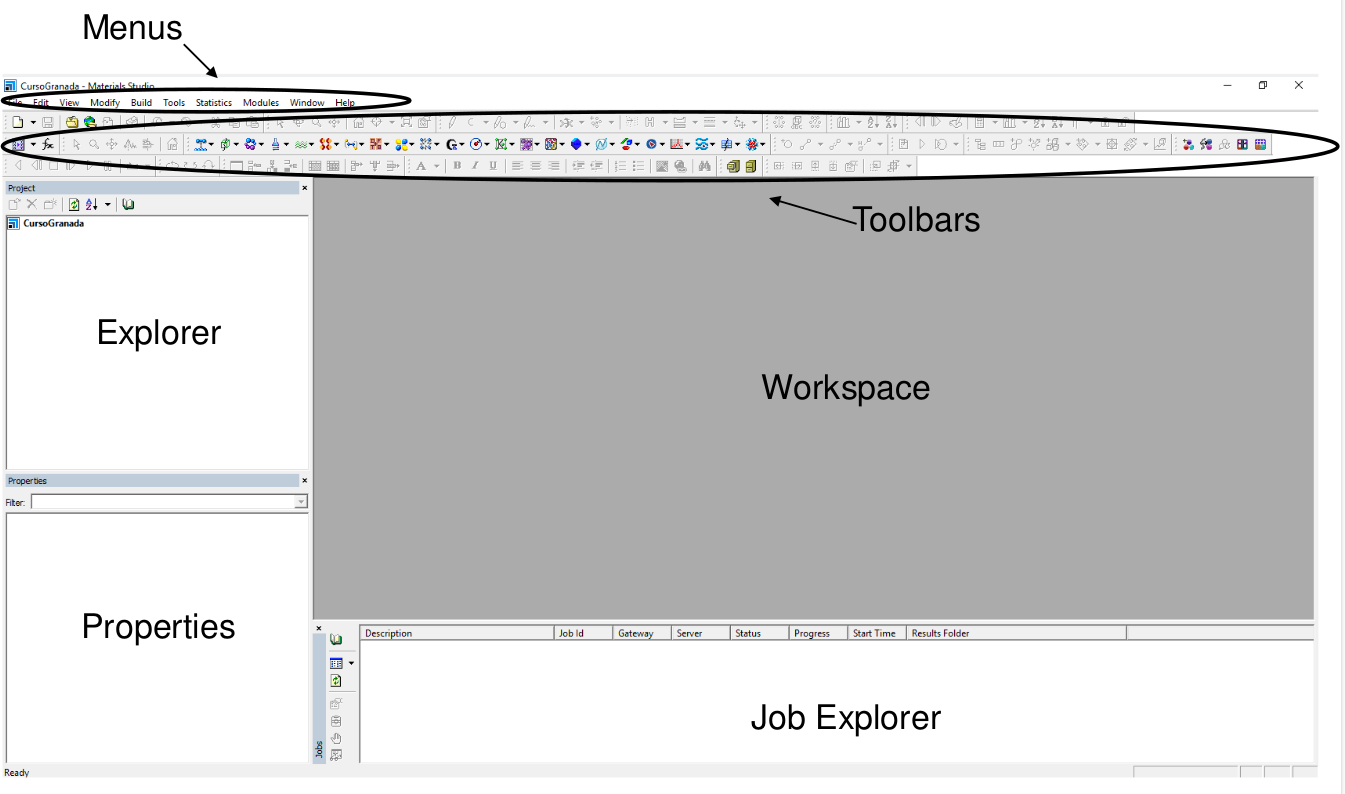
\includegraphics[height=2.45in,width=4.10in,viewport=0 0 1340 800,clip]{Figures/MS-Frame.png}
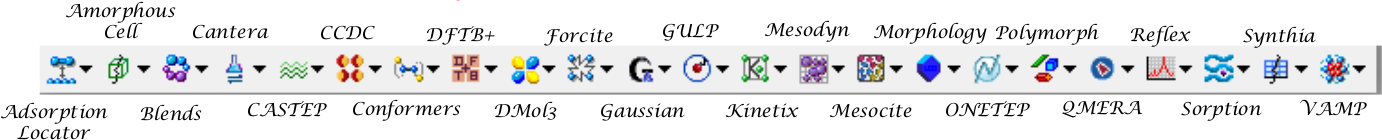
\includegraphics[height=0.45in,width=4.15in,viewport=0 0 1400 147,clip]{Figures/MS-Frame_calculators.png}
\caption{\tiny \textrm{The frame of Materials studio.}}%(与文献\cite{EPJB33-47_2003}图1对比)
\label{MS-Frame}
\end{figure}
}

%\subsection{\rm{Materials Studio:~Building}}
%\frame
%{
%	\frametitle{\textrm{MS:~Building Modules}}
%\begin{figure}[h!]
%\centering
%%\vspace*{-0.10in}
%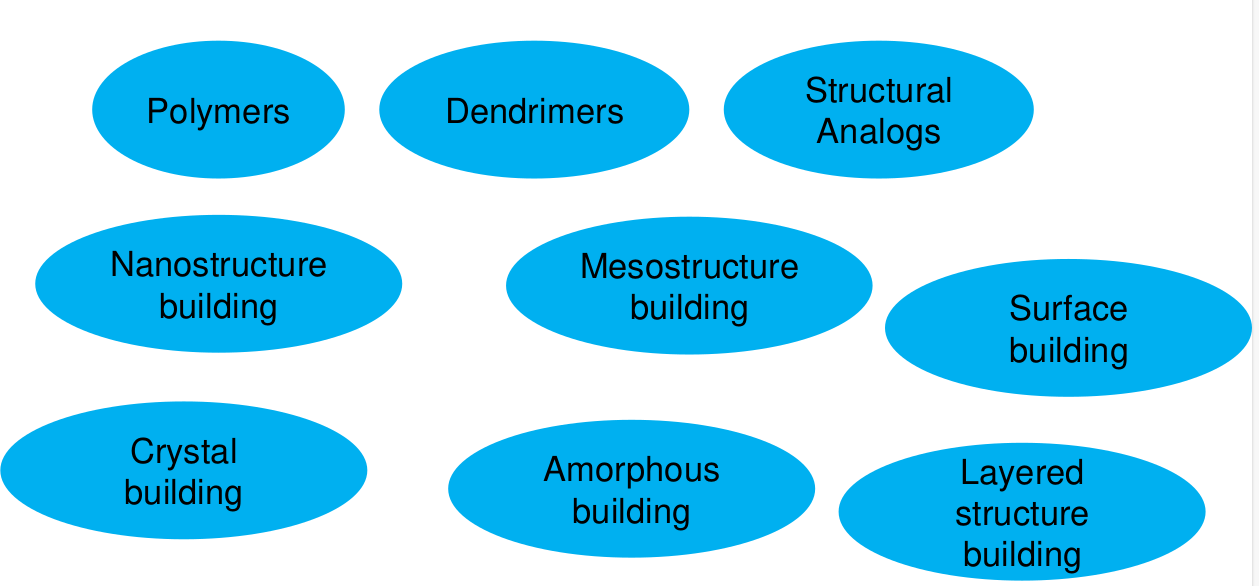
\includegraphics[height=1.90in,width=4.10in,viewport=0 0 1259 586,clip]{Figures/MS-Building_tools.png}
%\caption{\tiny \textrm{The Building tools in Materials studio.}}%(与文献\cite{EPJB33-47_2003}图1对比)
%\label{MS-Building-tools}
%\end{figure}
%}

%\subsection{\rm{Materials Studio:~Calculator}}
%\frame
%{
%	\frametitle{\textrm{MS:~Calculator}}
%\begin{figure}[h!]
%\centering
%\vspace*{-0.15in}
%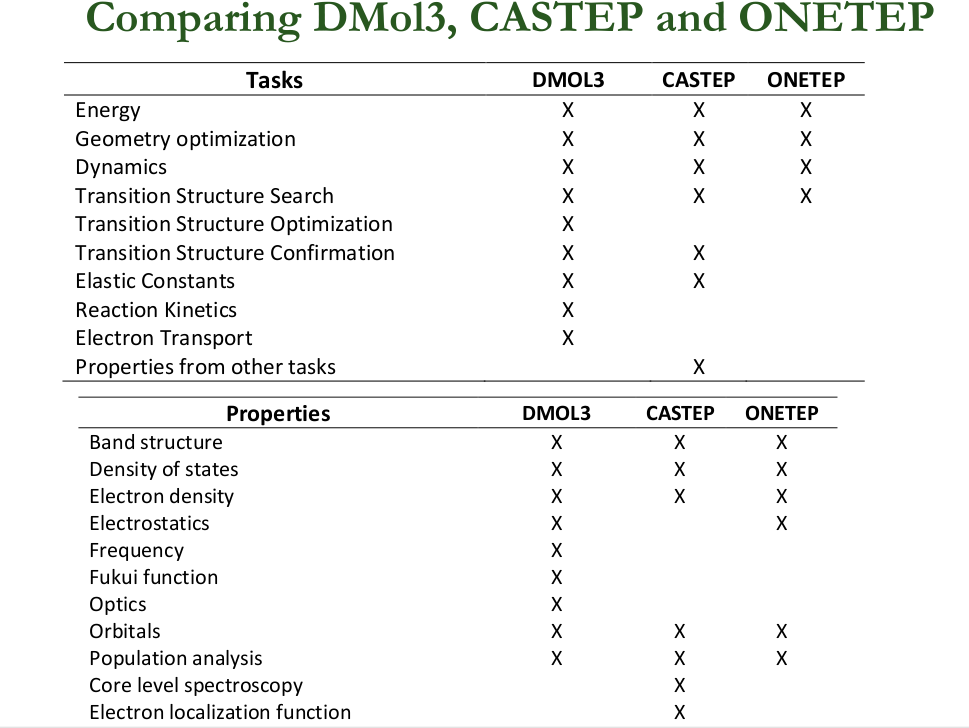
\includegraphics[height=2.75in,width=3.80in,viewport=0 0 969 728,clip]{Figures/MS-Caluculator-compare-2.png}
%\caption{\tiny \textrm{Comparing of Calculators in Materials studio.}}%(与文献\cite{EPJB33-47_2003}图1对比)
%\label{MS-Calculator-compare-2}
%\end{figure}
%}
%
%\frame
%{
%	\frametitle{\textrm{MS:~Calculator}}
%\begin{figure}[h!]
%\centering
%%\vspace*{-0.10in}
%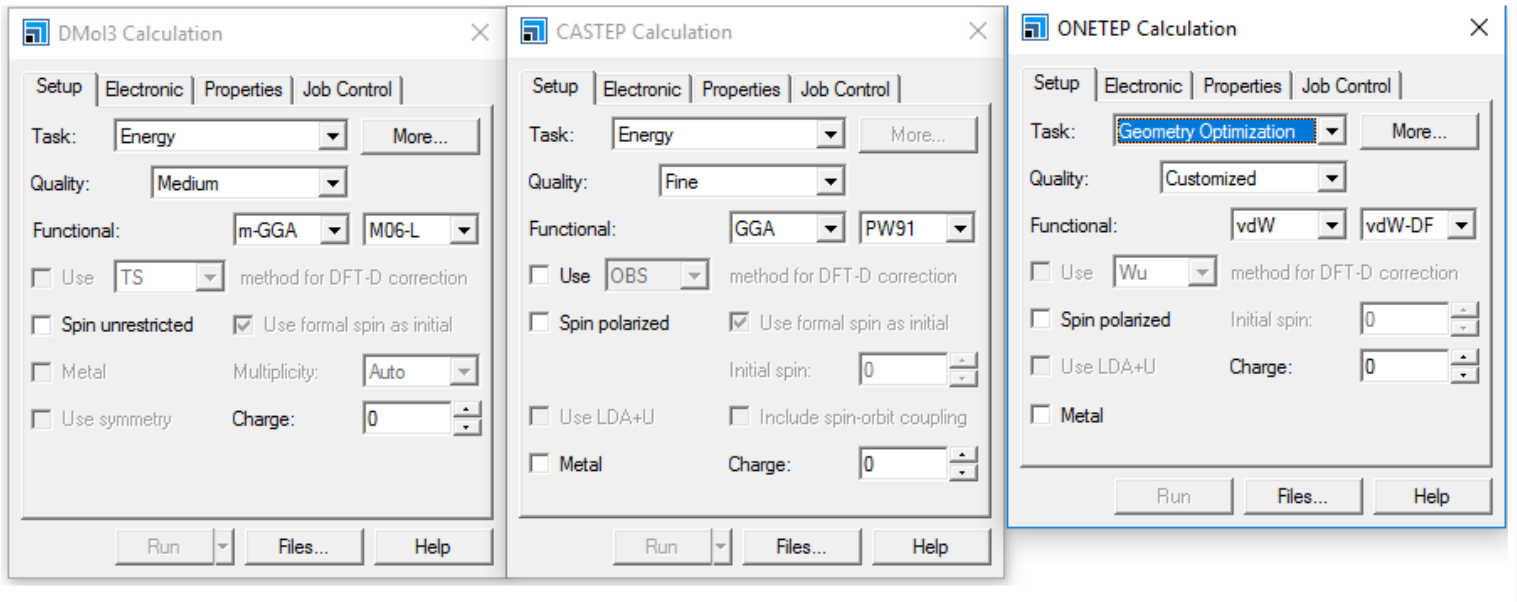
\includegraphics[height=1.50in,width=4.10in,viewport=0 0 1517 602,clip]{Figures/MS-Caluculator-compare-1.png}
%\caption{\tiny \textrm{Calculators in Materials studio:~parameters.}}%(与文献\cite{EPJB33-47_2003}图1对比)
%\label{MS-Calculator-compare-1}
%\end{figure}
%}
%
%\frame
%{
%	\frametitle{\textrm{MS:~XC-functionals}}
%\begin{figure}[h!]
%\centering
%\vspace*{-0.10in}
%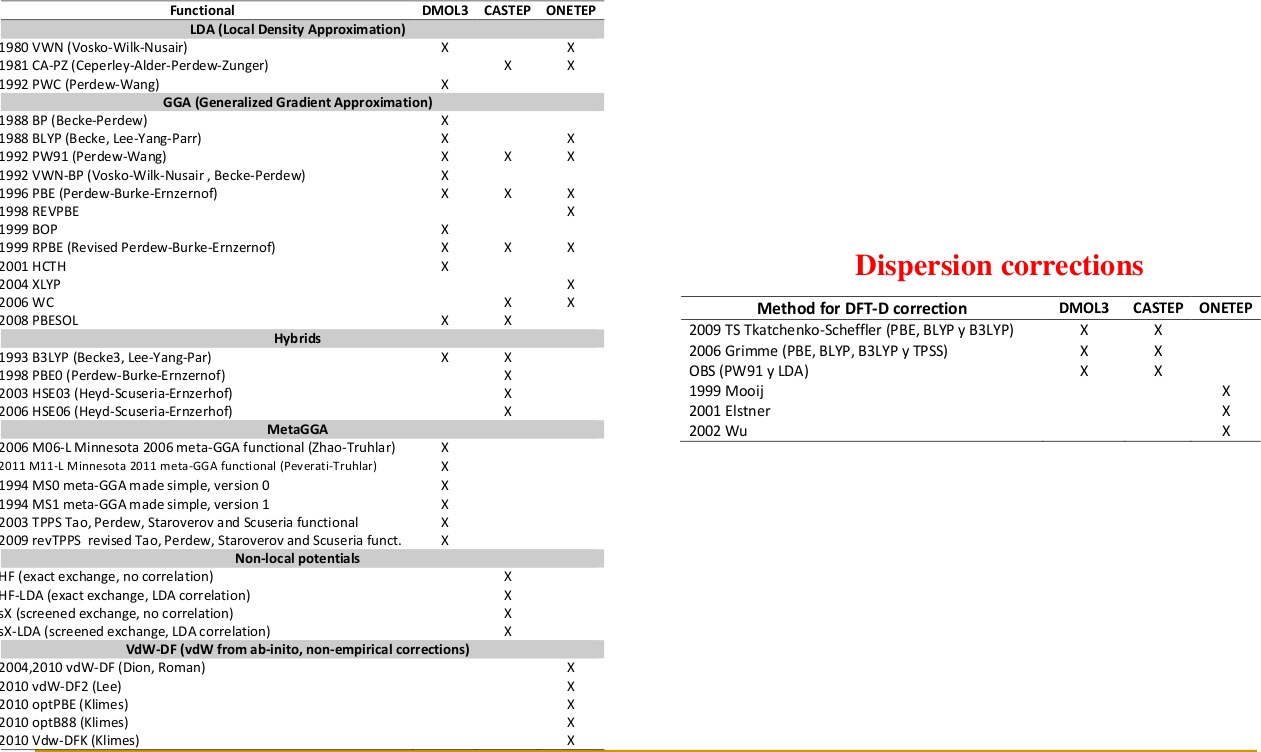
\includegraphics[height=2.50in,width=4.10in,viewport=0 0 1261 752,clip]{Figures/MS-xc_functional-compare.png}
%\caption{\tiny \textrm{XC-functionals in Materials studio.}}%(与文献\cite{EPJB33-47_2003}图1对比)
%\label{MS-xc_functional-compare}
%\end{figure}
%}
%
\frame
{
	\frametitle{\textrm{MS}的界面框架:~\textrm{Indigo}}
\begin{figure}[h!]
\centering
\vspace*{-0.28in}
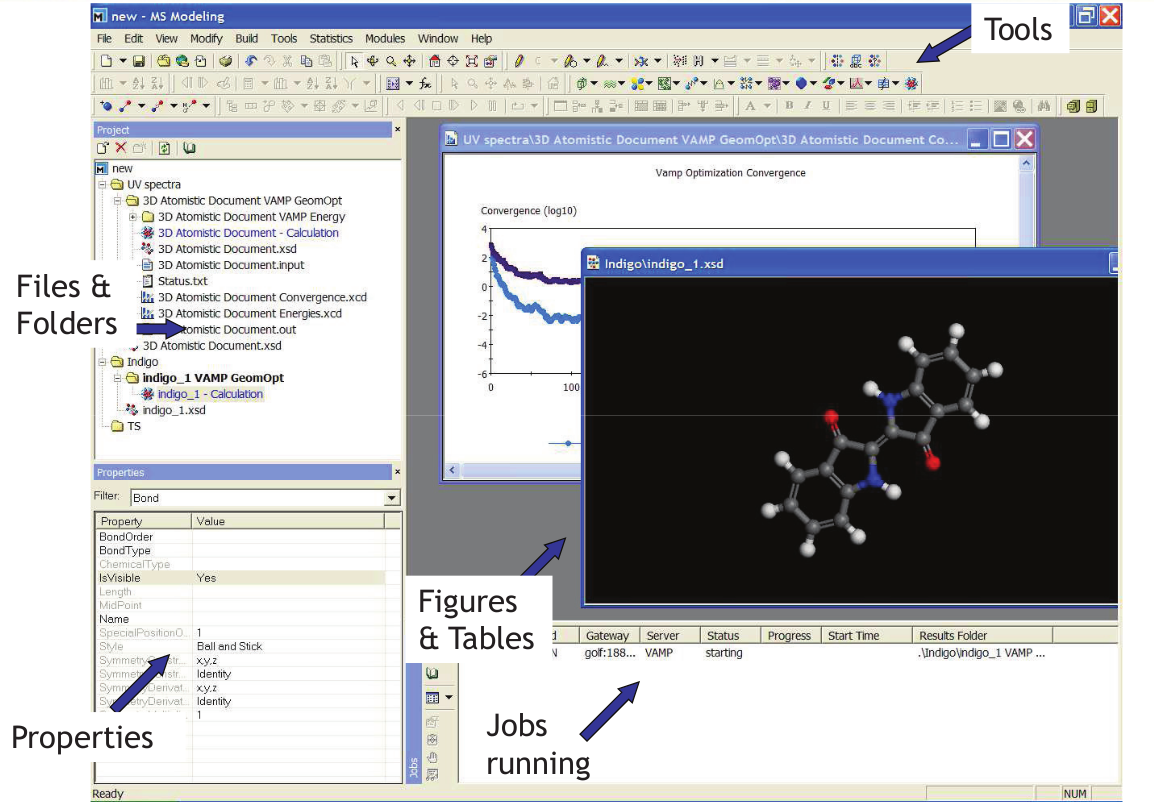
\includegraphics[height=2.85in,width=4.15in,viewport=0 0 1140 800,clip]{Figures/MS-Frame_example.png}
\caption{\tiny \textrm{The frame of Materials studio:~Example Indigo.}}%(与文献\cite{EPJB33-47_2003}图1对比)
\label{MS-Frame_example}
\end{figure}
}

\subsection{\rm{Materials Studio:~Quick Start}}
\frame
{
	\frametitle{\textrm{MS:~Quick Start-01}}
\begin{figure}[h!]
\centering
\vspace*{-0.21in}
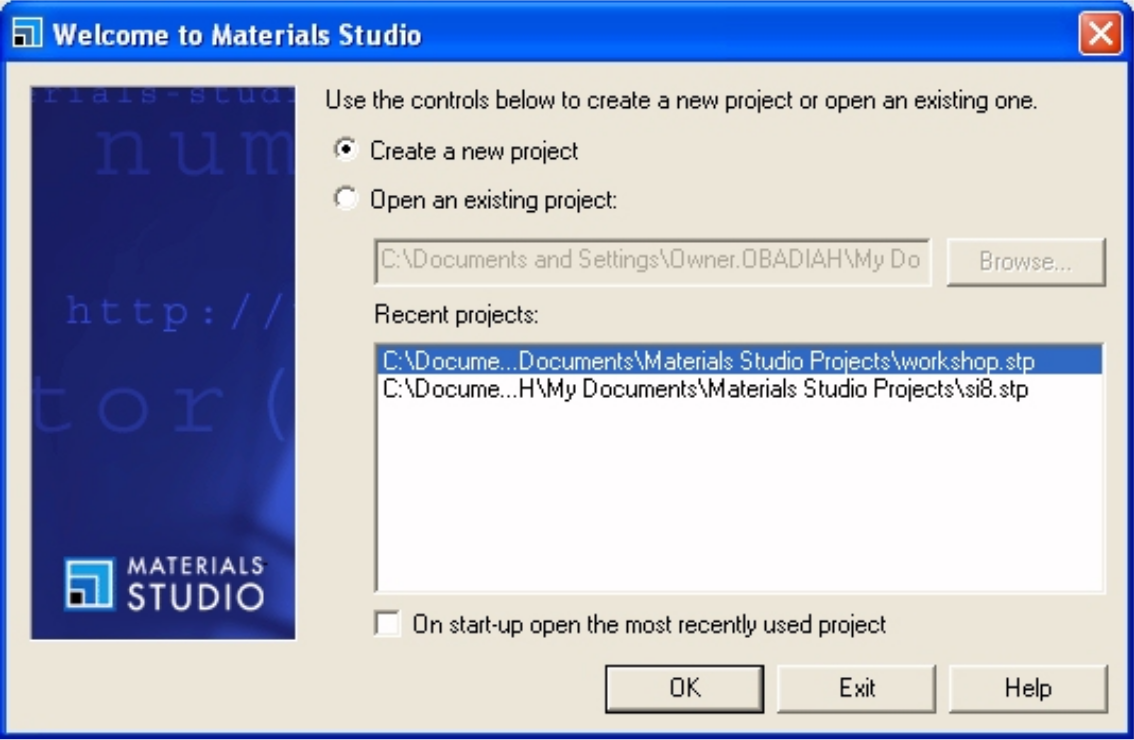
\includegraphics[height=2.70in,width=4.10in,viewport=0 0 1134 740,clip]{Figures/MS-New_Project-01.png}
\caption{\tiny \textrm{Quick Start for Materials studio:~Step-01.}}%(与文献\cite{EPJB33-47_2003}图1对比)
\label{MS-Quick_Start-01}
\end{figure}
}

\frame
{
	\frametitle{\textrm{MS:~Quick Start-02}}
\begin{figure}[h!]
\centering
\vspace*{-0.10in}
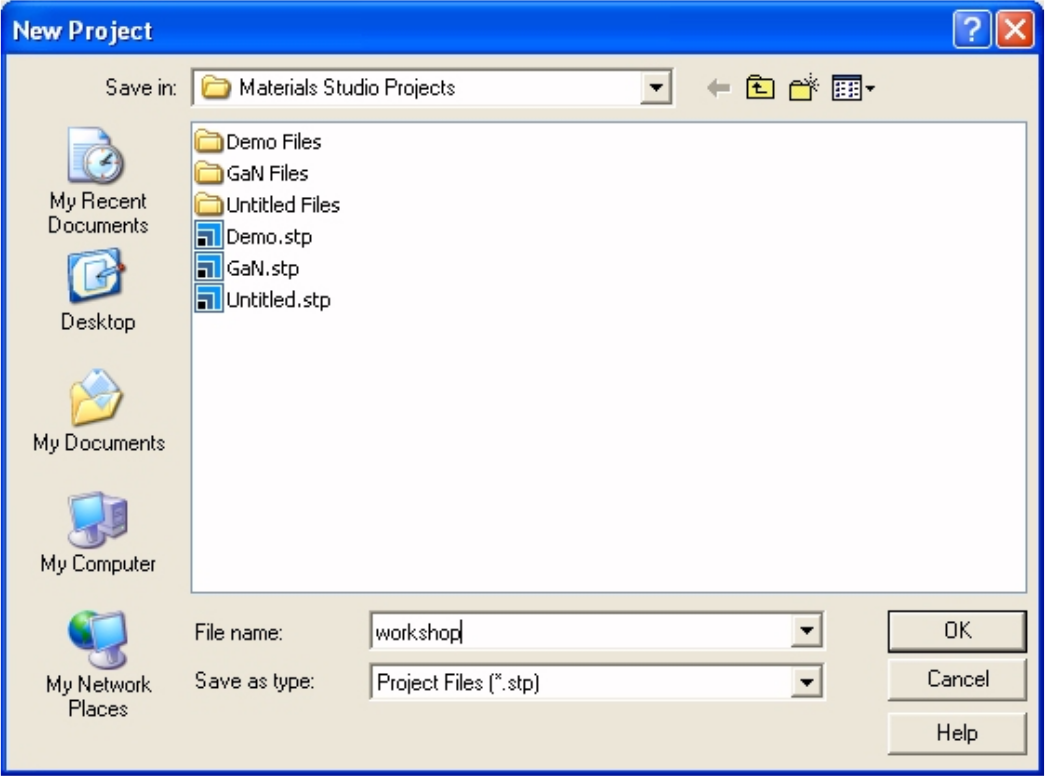
\includegraphics[height=2.70in,width=4.00in,viewport=0 0 1045 776,clip]{Figures/MS-New_Project-02.png}
\caption{\tiny \textrm{Quick Start for Materials studio:~Step-02.}}%(与文献\cite{EPJB33-47_2003}图1对比)
\label{MS-Quick_Start-02}
\end{figure}
}

\frame
{
	\frametitle{\textrm{MS:~Quick Start-03}}
\begin{figure}[h!]
\centering
\vspace*{-0.10in}
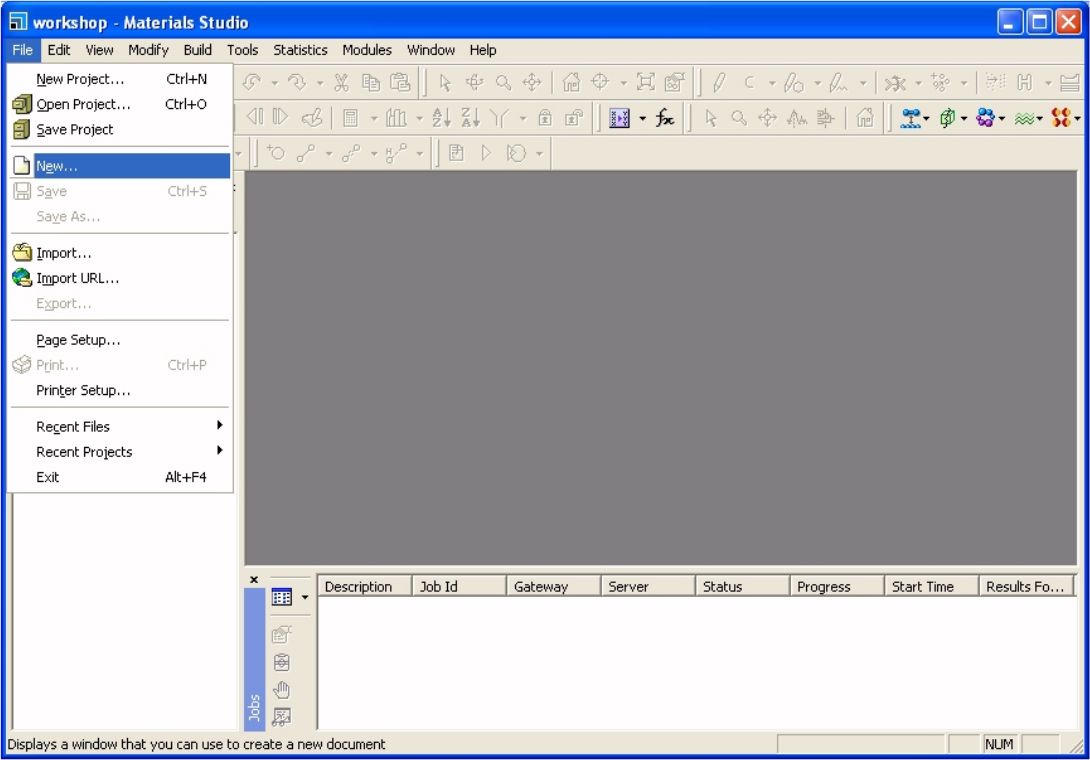
\includegraphics[height=2.68in,width=4.00in,viewport=0 0 1090 760,clip]{Figures/MS-New_Project-03.png}
\caption{\tiny \textrm{Quick Start for Materials studio:~Step-03.}}%(与文献\cite{EPJB33-47_2003}图1对比)
\label{MS-Quick_Start-03}
\end{figure}
}

\subsection{\rm{Materials Studio:~Modelling}}
\frame
{
	\frametitle{\textrm{MS:~Quick Start-Modelling-01}}
\begin{figure}[h!]
\centering
\vspace*{-0.10in}
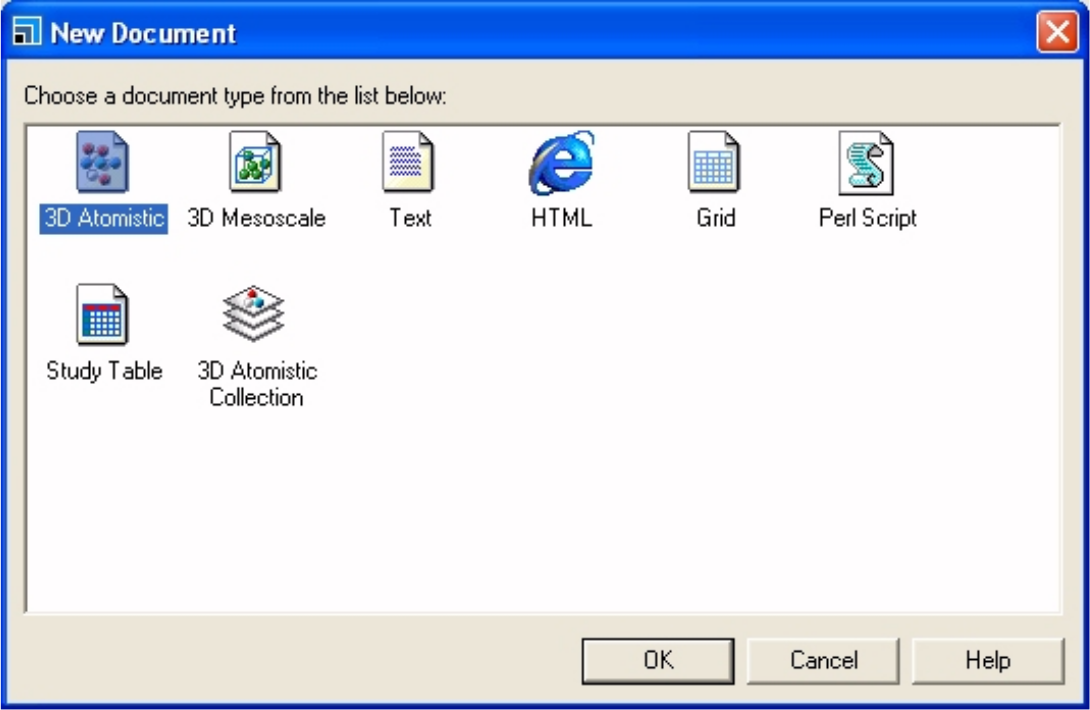
\includegraphics[height=2.60in,width=4.00in,viewport=0 0 1090 710,clip]{Figures/MS-New_Project-04.png}
\caption{\tiny \textrm{Quick Start for Materials studio:~Modelling-01.}}%(与文献\cite{EPJB33-47_2003}图1对比)
\label{MS-Quick_Start-Modelling-01}
\end{figure}
}

\frame
{
	\frametitle{\textrm{MS:~Quick Start-Modelling-02}}
\begin{figure}[h!]
\centering
\vspace*{-0.10in}
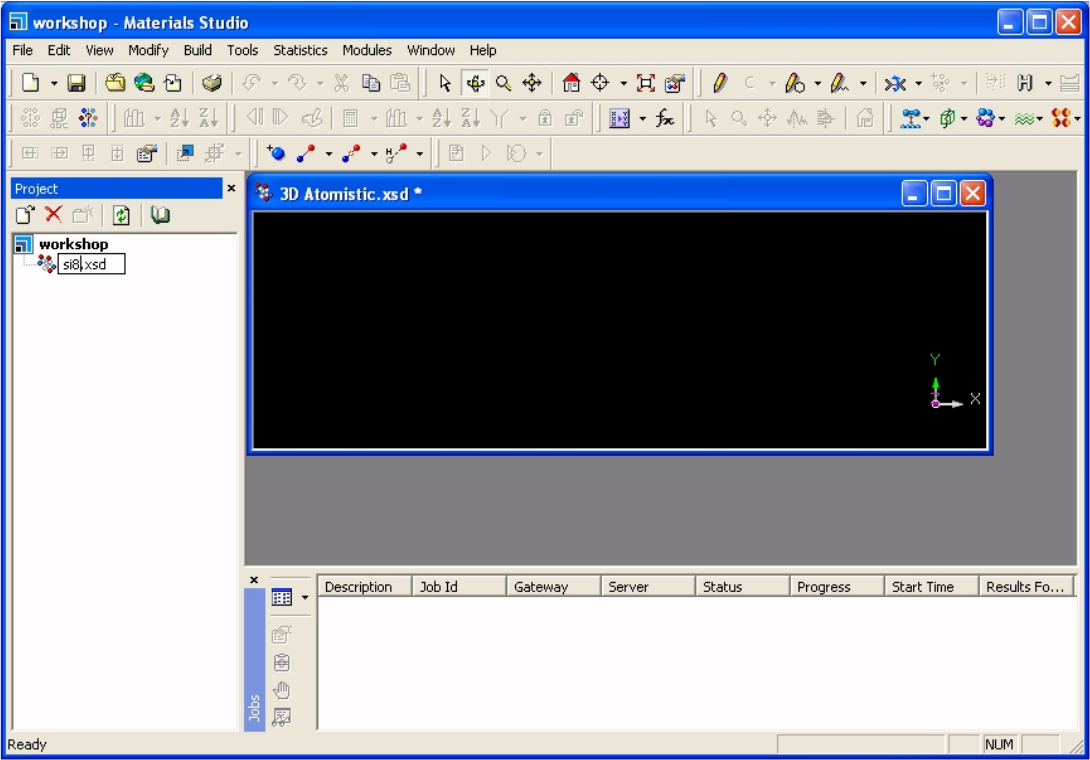
\includegraphics[height=2.68in,width=4.00in,viewport=0 0 1090 760,clip]{Figures/MS-New_Project-05.png}
\caption{\tiny \textrm{Quick Start for Materials studio:~Modelling-02.}}%(与文献\cite{EPJB33-47_2003}图1对比)
\label{MS-Quick_Start-Modelling-02}
\end{figure}
}

\frame
{
	\frametitle{\textrm{MS:~Modelling Crystal-01}}
\begin{figure}[h!]
\centering
\vspace*{-0.10in}
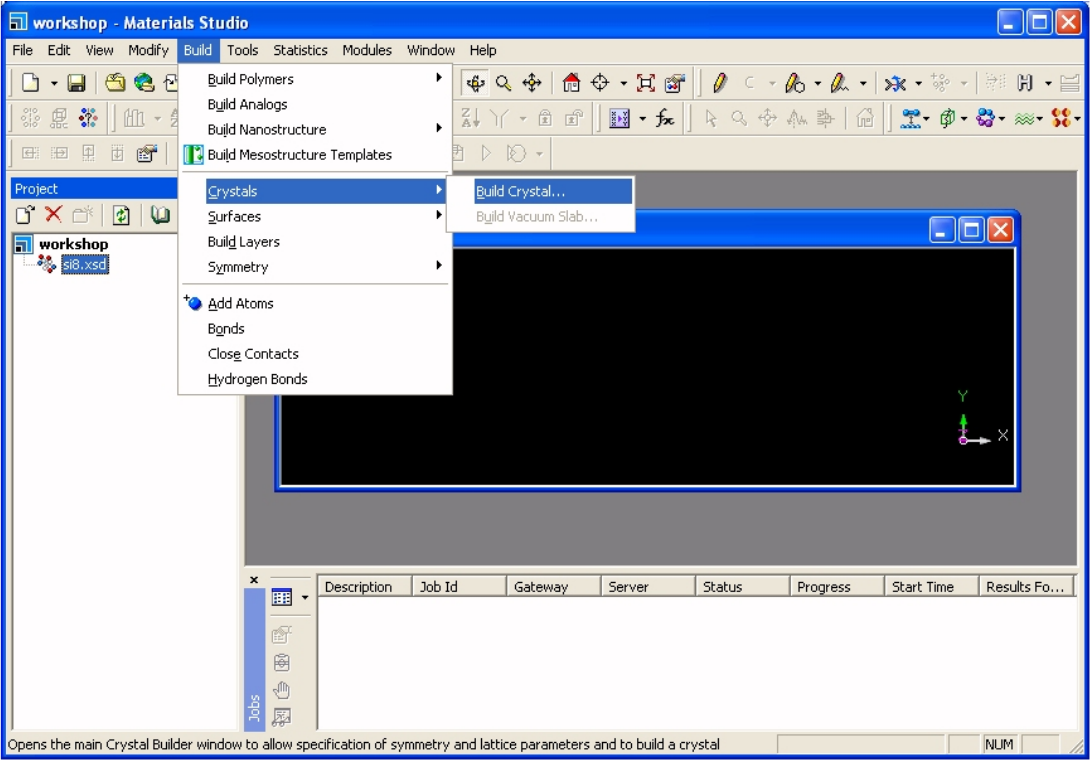
\includegraphics[height=2.68in,width=4.00in,viewport=0 0 1090 760,clip]{Figures/MS-New_Project-06.png}
\caption{\tiny \textrm{Modelling crystal by Materials studio.}}%(与文献\cite{EPJB33-47_2003}图1对比)
\label{MS-Modelling-Crystal-01}
\end{figure}
}

\frame
{
	\frametitle{\textrm{MS:~Modelling Crystal-02}}
\begin{figure}[h!]
\centering
\vspace*{-0.15in}
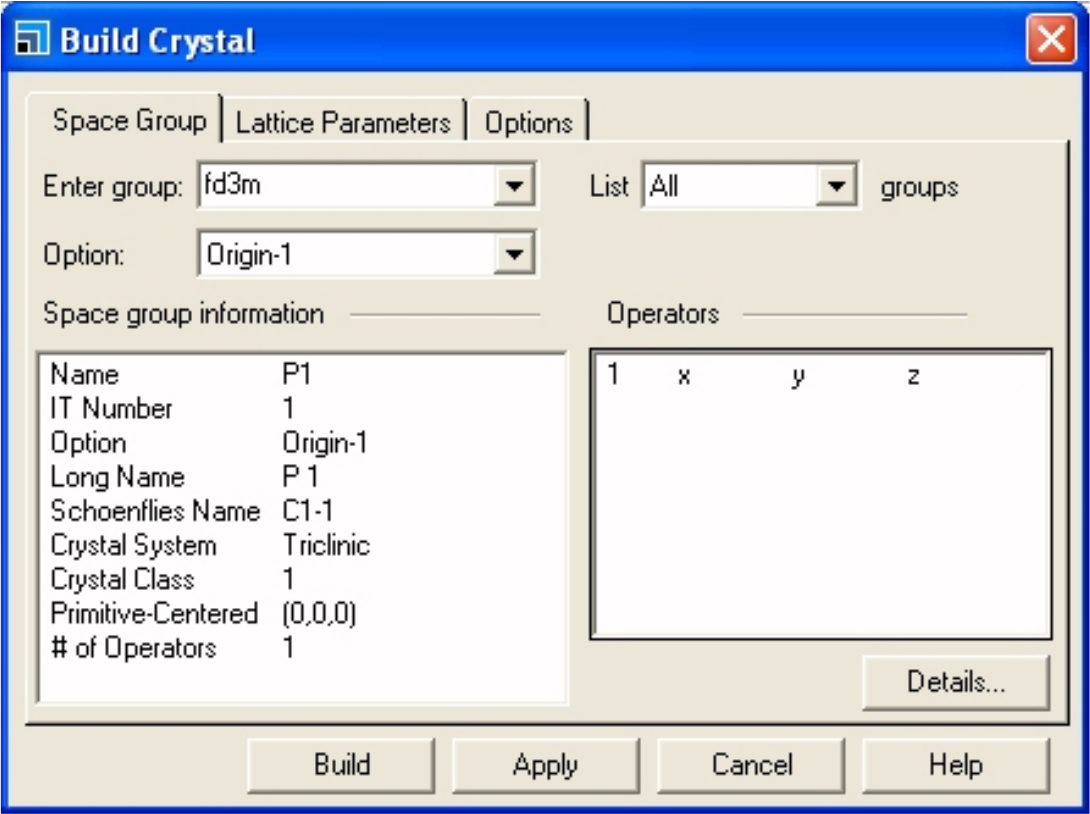
\includegraphics[height=2.75in,width=4.00in,viewport=0 0 1090 814,clip]{Figures/MS-New_Project-07.png}
\caption{\tiny \textrm{Modelling crystal by Materials studio:~Parameters.}}%(与文献\cite{EPJB33-47_2003}图1对比)
\label{MS-Modelling-Crystal-02}
\end{figure}
}

\frame
{
	\frametitle{\textrm{MS:~Modelling Crystal-03}}
\begin{figure}[h!]
\centering
\vspace*{-0.15in}
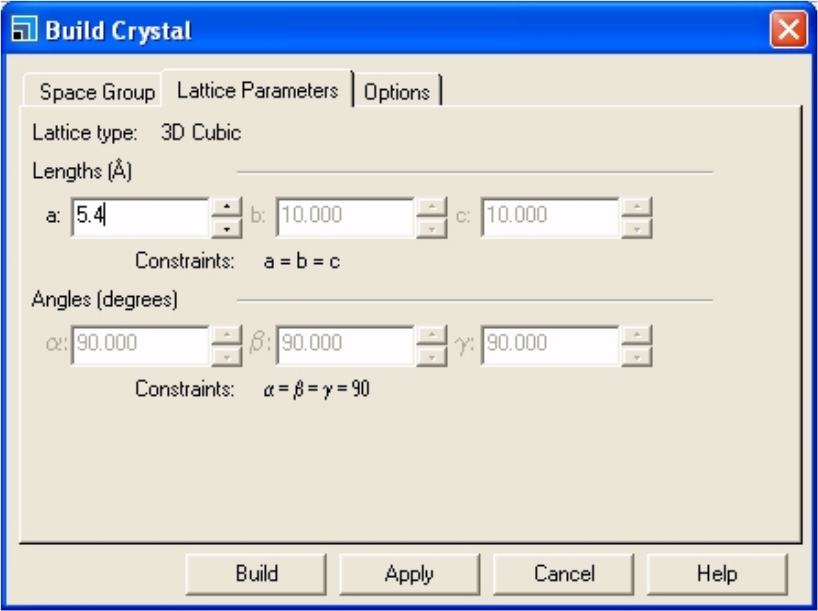
\includegraphics[height=2.75in,width=3.70in,viewport=0 0 818 616,clip]{Figures/MS-New_Project-08.png}
\caption{\tiny \textrm{Modelling crystal by Materials studio:~Lattice-parameters.}}%(与文献\cite{EPJB33-47_2003}图1对比)
\label{MS-Modelling-Crystal-03}
\end{figure}
}

\frame
{
	\frametitle{\textrm{MS:~Modelling Crystal-04}}
\begin{figure}[h!]
\centering
\vspace*{-0.10in}
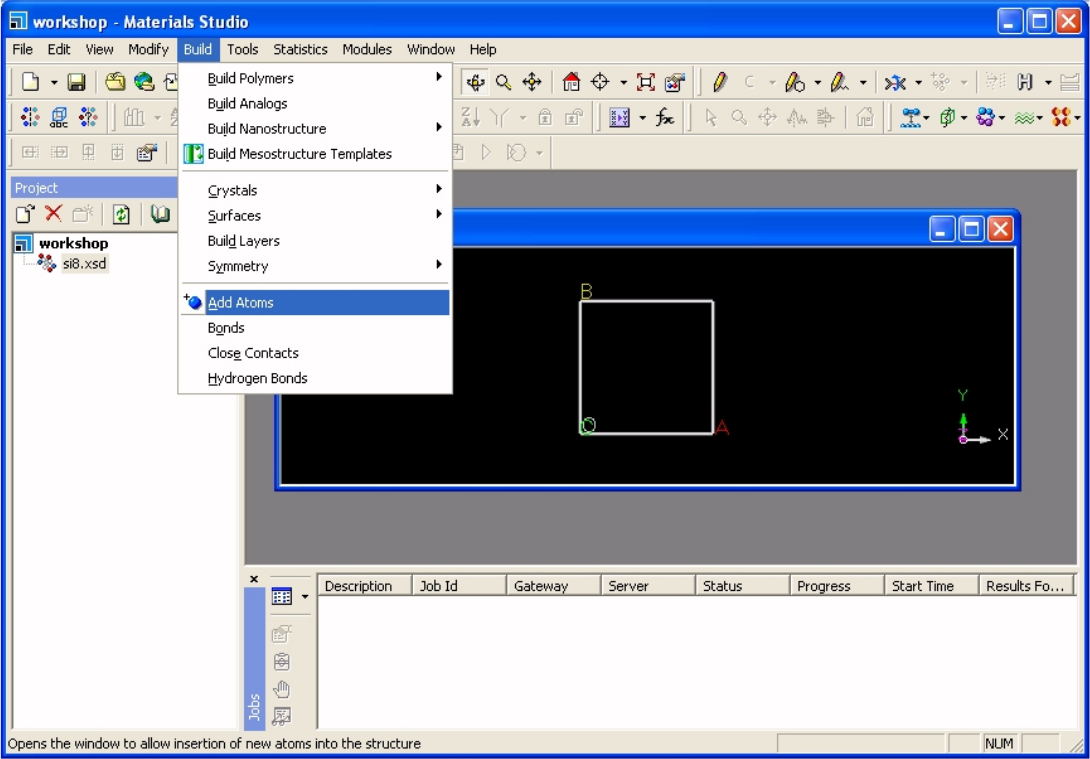
\includegraphics[height=2.70in,width=4.00in,viewport=0 0 1090 759,clip]{Figures/MS-New_Project-09.png}
\caption{\tiny \textrm{Modelling crystal by Materials studio:~Elements.}}%(与文献\cite{EPJB33-47_2003}图1对比)
\label{MS-Modelling-Crystal-04}
\end{figure}
}

\frame
{
	\frametitle{\textrm{MS:~Modelling Crystal example:~Si}}
\begin{figure}[h!]
\centering
\vspace*{-0.10in}
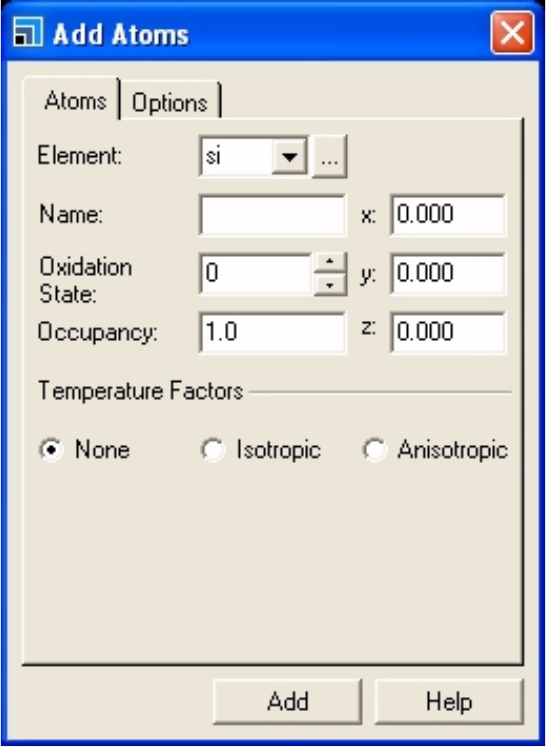
\includegraphics[height=2.70in,width=2.30in,viewport=0 0 546 747,clip]{Figures/MS-New_Project-10-Si_example.png}
\caption{\tiny \textrm{Modelling crystal by Materials studio:~Si.}}%(与文献\cite{EPJB33-47_2003}图1对比)
\label{MS-Modelling-Crystal-05}
\end{figure}
}

\frame
{
	\frametitle{\textrm{MS:~Modelling Crystal example:~Si}}
\begin{figure}[h!]
\centering
\vspace*{-0.10in}
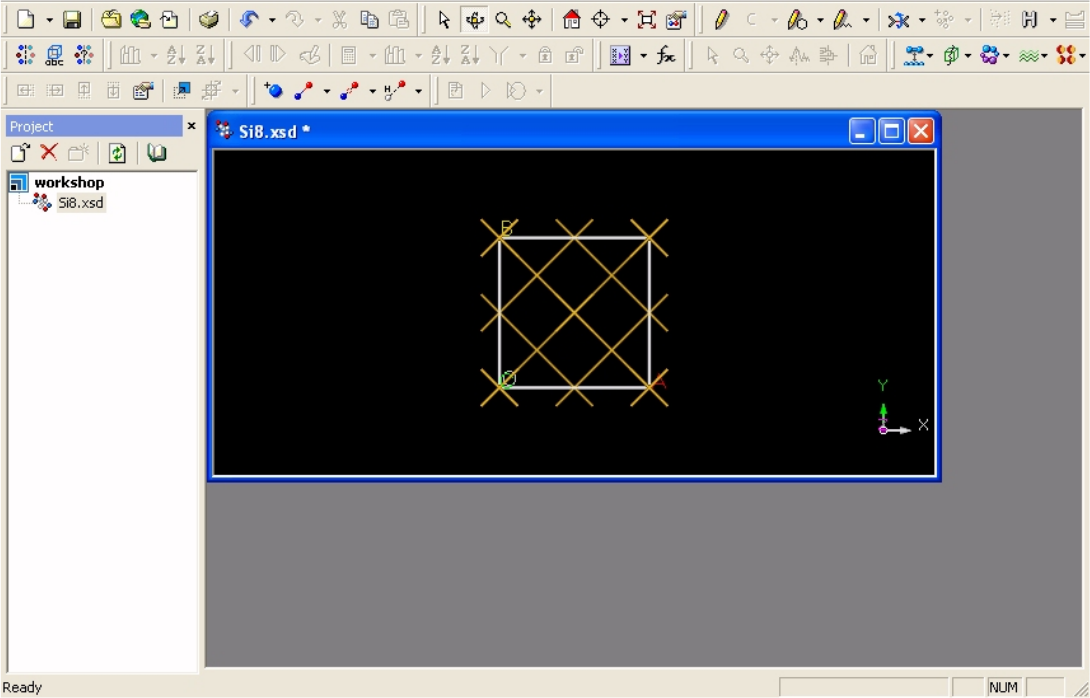
\includegraphics[height=2.65in,width=4.00in,viewport=0 0 1090 698,clip]{Figures/MS-New_Project-11-Si_crystal.png}
\caption{\tiny \textrm{Modelling crystal by Materials studio:~Si.}}%(与文献\cite{EPJB33-47_2003}图1对比)
\label{MS-Modelling-Crystal-06}
\end{figure}
}

\subsection{\rm{Materials Studio:~Calculation}}
\frame
{
	\frametitle{\textrm{MS:~CASTEP Calculation example:~Si}}
\begin{figure}[h!]
\centering
\vspace*{-0.10in}
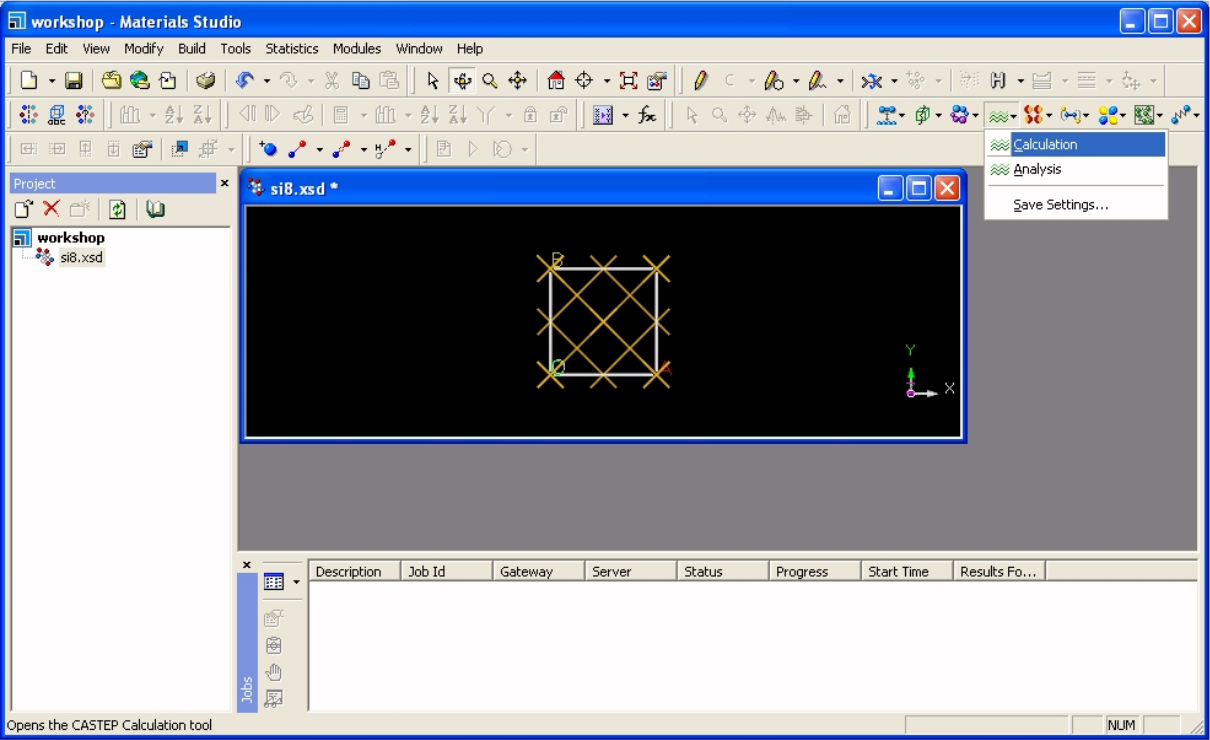
\includegraphics[height=2.62in,width=4.00in,viewport=0 0 1210 740,clip]{Figures/MS-CASTEP-01-Si.png}
\caption{\tiny \textrm{CASTEP Calculation by Materials studio:~Si.}}%(与文献\cite{EPJB33-47_2003}图1对比)
\label{MS-CASTEP-Calculation-01}
\end{figure}
}

\frame
{
	\frametitle{\textrm{MS:~CASTEP Calculation example:~Si}}
\begin{figure}[h!]
\centering
%\vspace*{-0.10in}
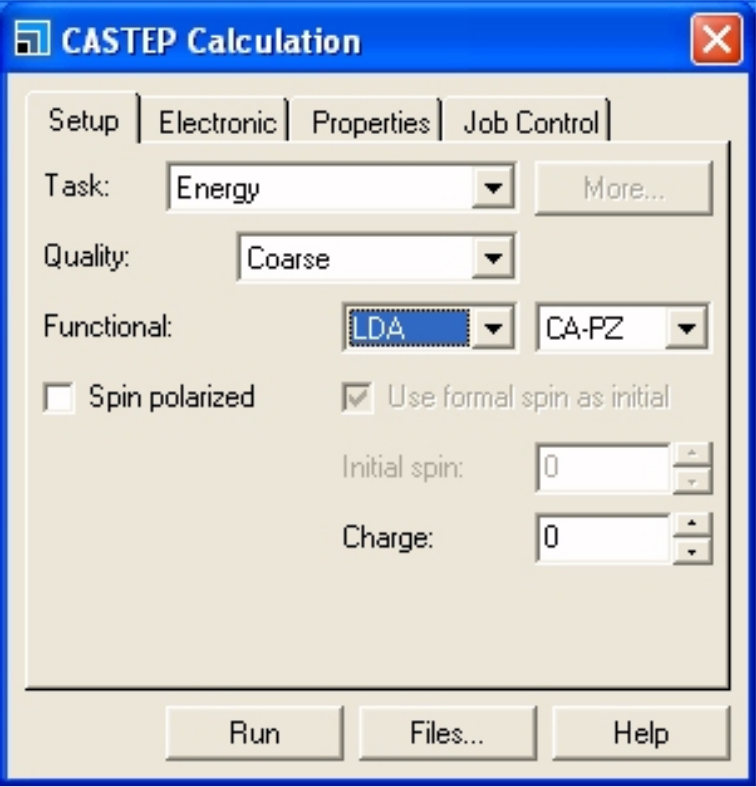
\includegraphics[height=2.05in,width=1.95in,viewport=0 0 756 787,clip]{Figures/MS-CASTEP-02-Si-parameter-1.png}
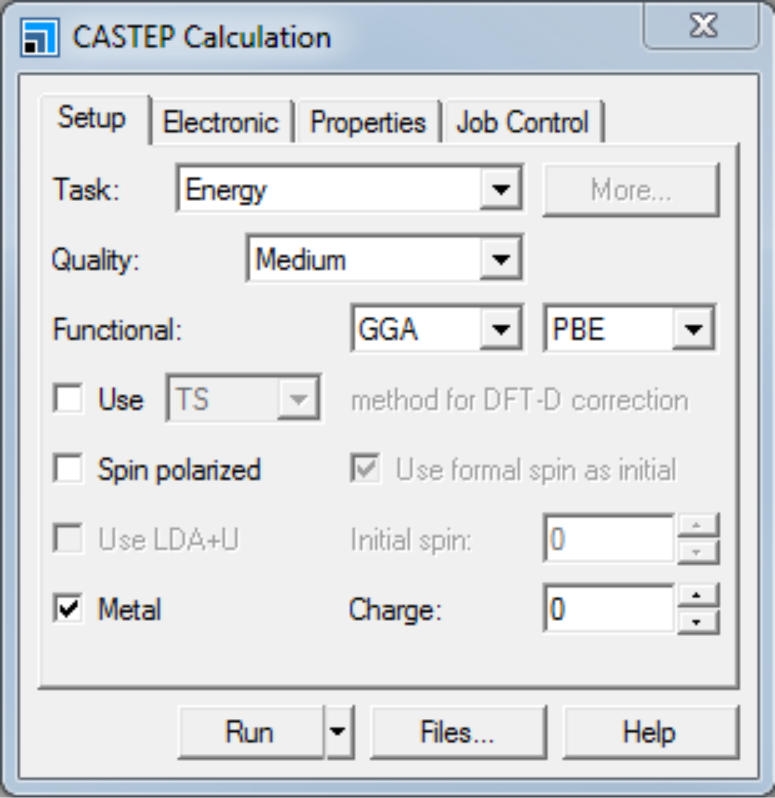
\includegraphics[height=2.05in,width=1.95in,viewport=0 0 775 798,clip]{Figures/MS-CASTEP-02-Si-parameter-2.png}
\caption{\tiny \textrm{CASTEP Calculation by Materials studio:~Parameter.}}%(与文献\cite{EPJB33-47_2003}图1对比)
\label{MS-CASTEP-Calculation-02}
\end{figure}
}

\frame
{
	\frametitle{\textrm{MS:~CASTEP Calculation example:~Si}}
\begin{figure}[h!]
\centering
\vspace*{-0.10in}
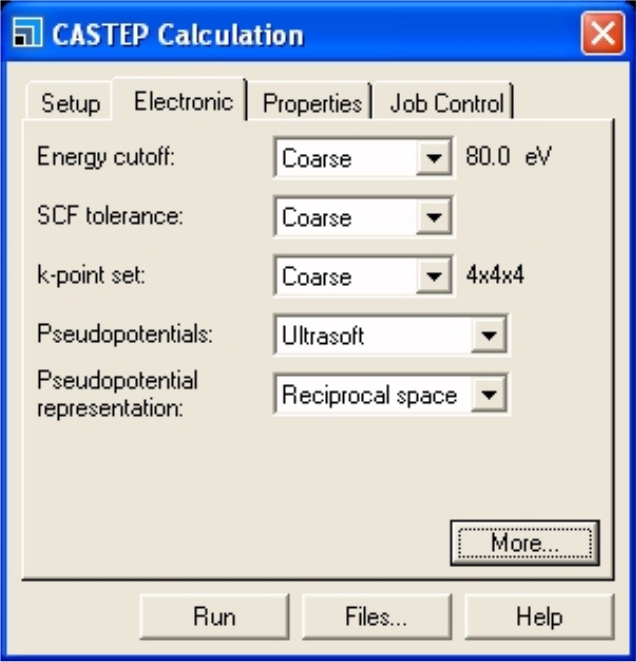
\includegraphics[height=2.15in,width=1.95in,viewport=0 -50 650 700,clip]{Figures/MS-CASTEP-13-Si-Calculat-Electron-step.png}
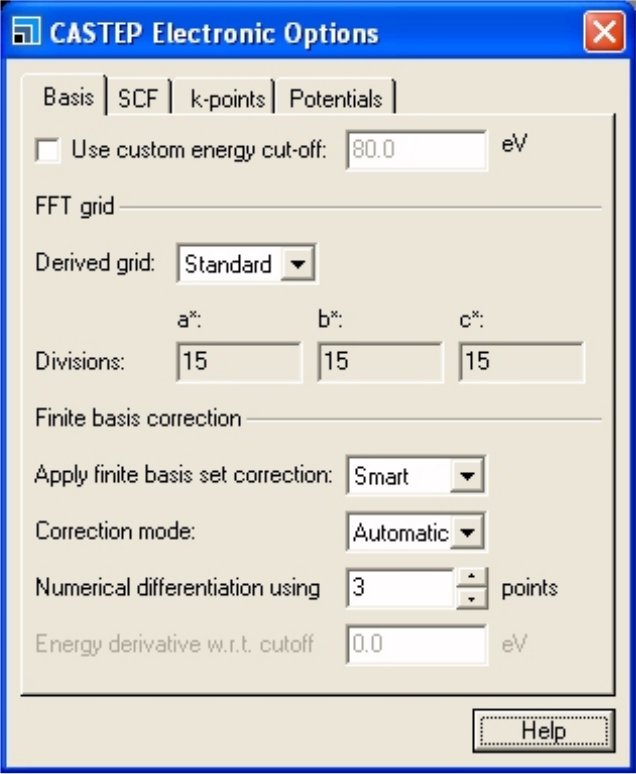
\includegraphics[height=2.15in,width=1.95in,viewport=0 0 636 774,clip]{Figures/MS-CASTEP-13-Si-Calculat-Electron-detail.png}
\caption{\tiny \textrm{CASTEP Calculation by Materials studio:~Electron-step.}}%(与文献\cite{EPJB33-47_2003}图1对比)
\label{MS-CASTEP-Calculation-electron}
\end{figure}
}

\frame
{
	\frametitle{\textrm{MS:~CASTEP Calculation example:~Si}}
\begin{figure}[h!]
\centering
%\vspace*{-0.10in}
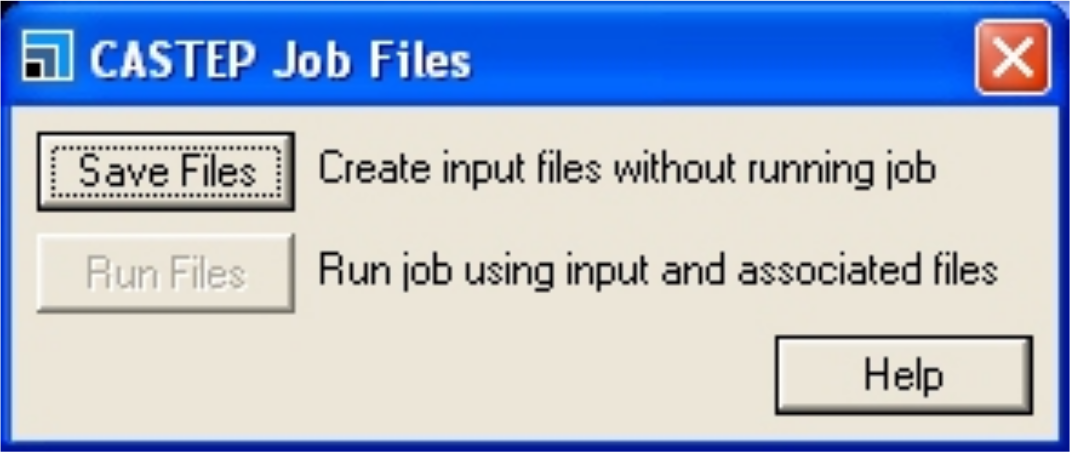
\includegraphics[height=1.15in,width=3.30in,viewport=0 0 1070 452,clip]{Figures/MS-CASTEP-03-Si-input-1.png}
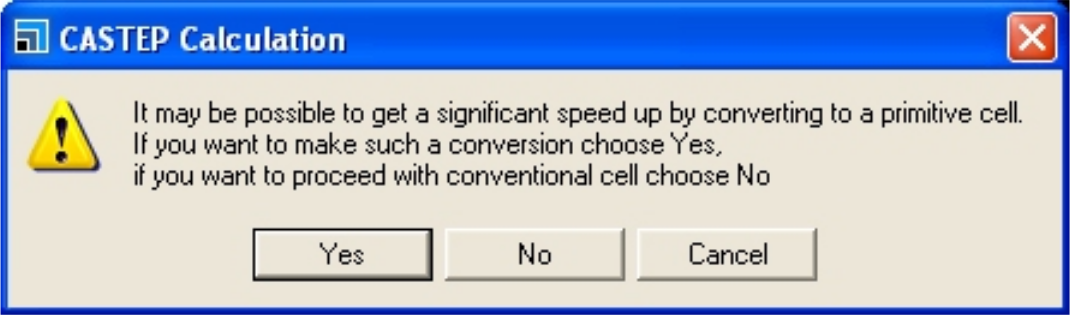
\includegraphics[height=1.15in,width=4.00in,viewport=0 0 1070 355,clip]{Figures/MS-CASTEP-03-Si-input-2.png}
\caption{\tiny \textrm{CASTEP Calculation.}}%(与文献\cite{EPJB33-47_2003}图1对比)
\label{MS-CASTEP-Calculation-03}
\end{figure}
}

\frame
{
	\frametitle{\textrm{MS:~CASTEP Calculation example:~Si}}
\begin{figure}[h!]
\centering
\vspace*{-0.10in}
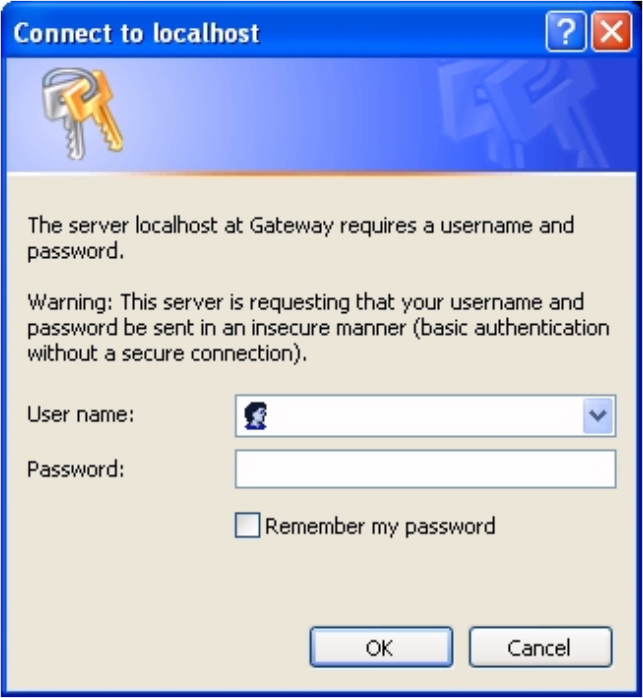
\includegraphics[height=2.65in,width=2.63in,viewport=0 0 643 698,clip]{Figures/MS-CASTEP-04-Si-sever.png}
\caption{\tiny \textrm{CASTEP Calculation by Materials studio:~Connect to localhost.}}%(与文献\cite{EPJB33-47_2003}图1对比)
\label{MS-CASTEP-Calculation-sever}
\end{figure}
}

\frame
{
	\frametitle{\textrm{MS:~CASTEP Calculation example:~Si}}
\begin{figure}[h!]
\centering
\vspace*{-0.10in}
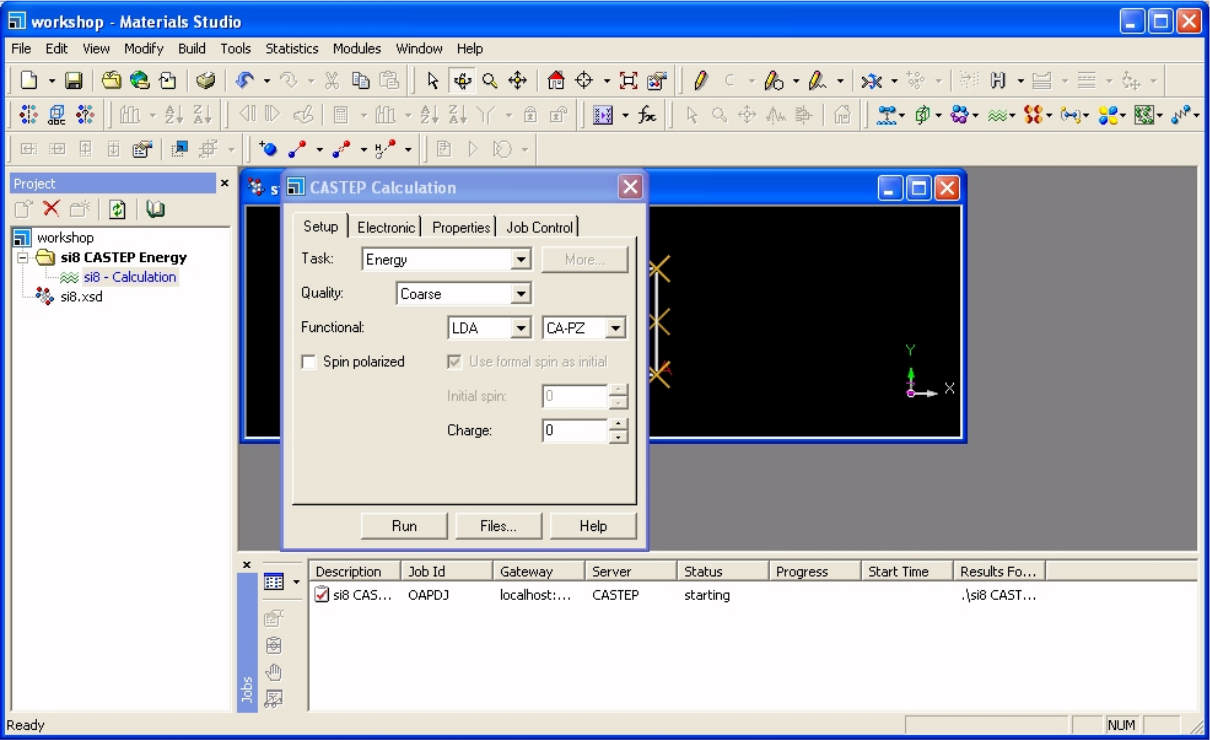
\includegraphics[height=2.60in,width=4.00in,viewport=0 0 1210 740,clip]{Figures/MS-CASTEP-05-Si-Calculat.png}
\caption{\tiny \textrm{CASTEP Calculation by Materials studio:~Run.}}%(与文献\cite{EPJB33-47_2003}图1对比)
\label{MS-CASTEP-Calculation-Run}
\end{figure}
}

\frame
{
	\frametitle{\textrm{MS:~CASTEP Calculation example:~Si}}
\begin{figure}[h!]
\centering
%\vspace*{-0.10in}
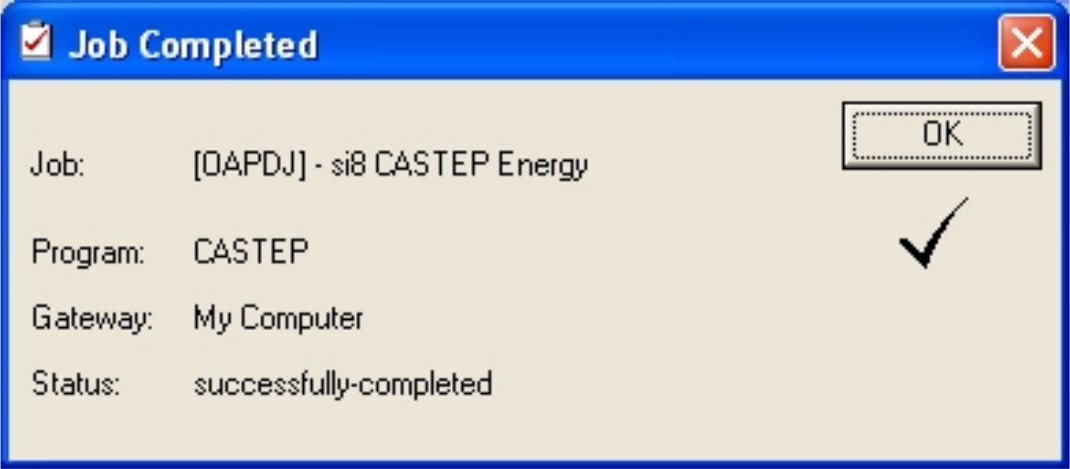
\includegraphics[height=1.50in,width=4.00in,viewport=0 0 1070 469,clip]{Figures/MS-CASTEP-06-Si-Calculat-finish.png}
\caption{\tiny \textrm{CASTEP Calculation by Materials studio:~Complete.}}%(与文献\cite{EPJB33-47_2003}图1对比)
\label{MS-CASTEP-Calculation-Complete}
\end{figure}
}

\frame
{
	\frametitle{\textrm{MS:~CASTEP Calculation example:~Si}}
\begin{figure}[h!]
\centering
\vspace*{-0.10in}
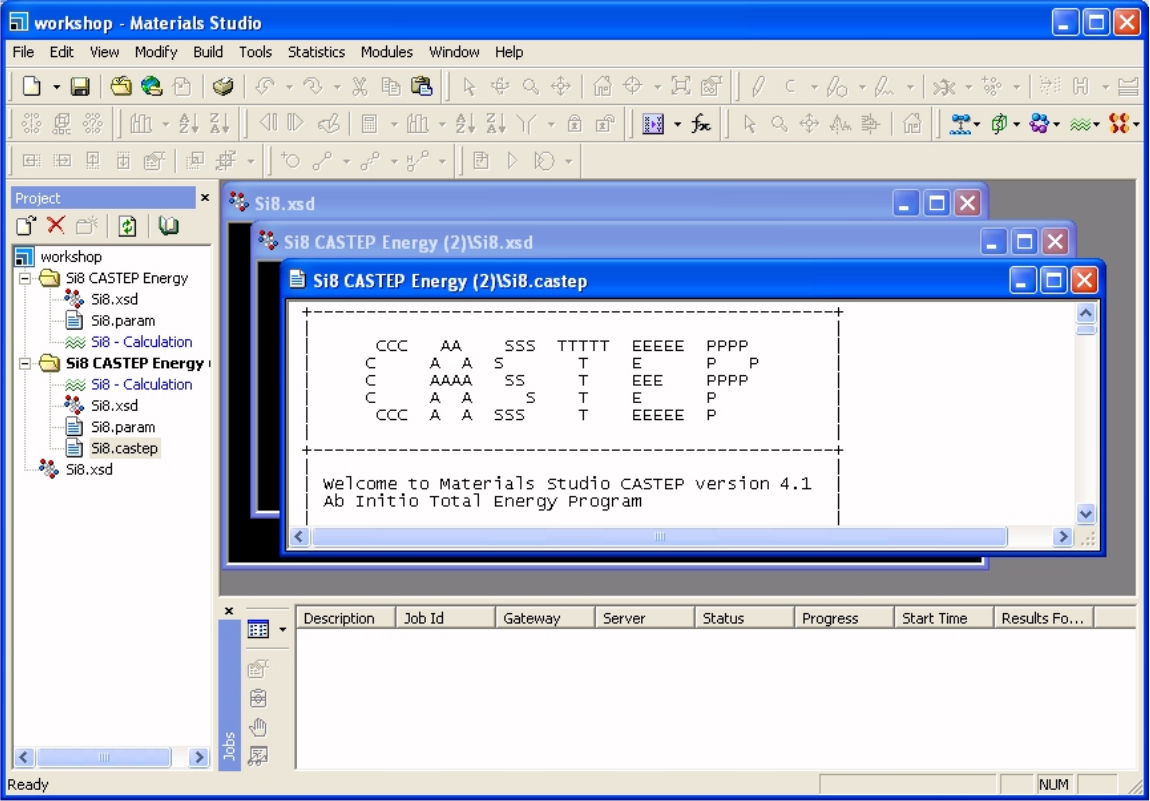
\includegraphics[height=2.66in,width=4.00in,viewport=0 0 1150 801,clip]{Figures/MS-CASTEP-07-Si-Calculat-data.png}
\caption{\tiny \textrm{CASTEP Calculation by Materials studio:~Finish.}}%(与文献\cite{EPJB33-47_2003}图1对比)
\label{MS-CASTEP-Calculation-data}
\end{figure}
}

\frame
{
	\frametitle{\textrm{MS:~CASTEP Calculation example:~Si}}
\begin{figure}[h!]
\centering
\vspace*{-0.10in}
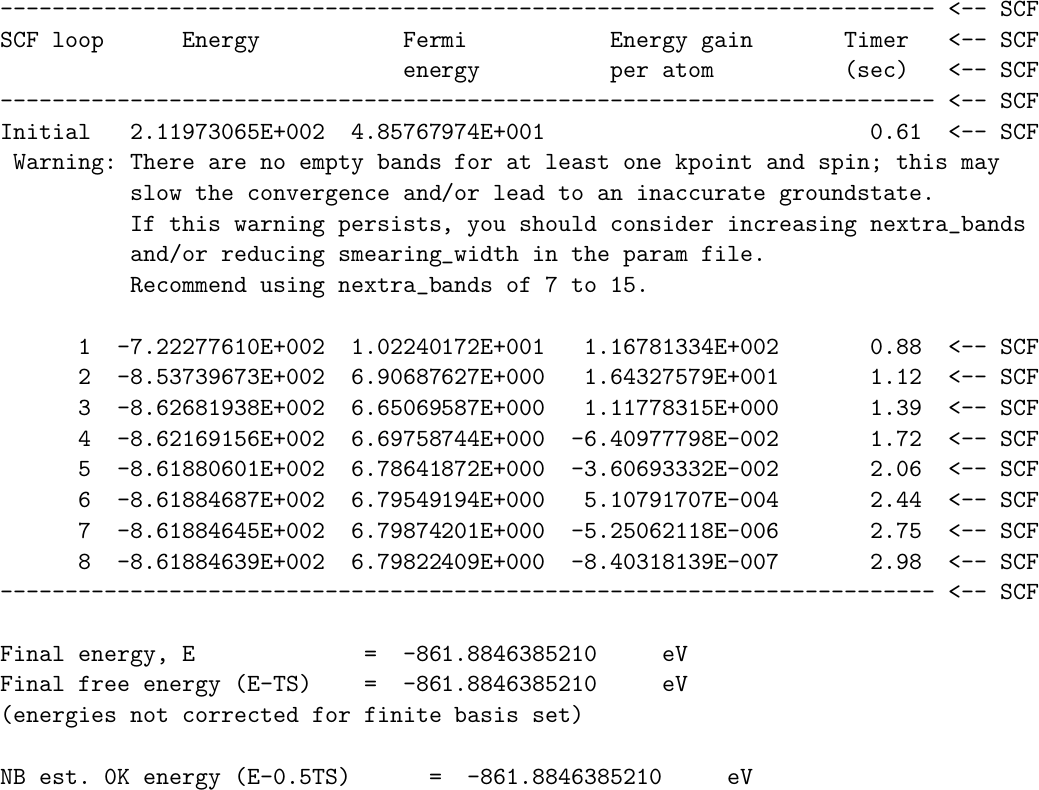
\includegraphics[height=2.60in,width=4.00in,viewport=0 0 1039 790,clip]{Figures/MS-CASTEP-08-Si-Calculat-SCF.png}
\caption{\tiny \textrm{CASTEP Calculation by Materials studio:~SCF.}}%(与文献\cite{EPJB33-47_2003}图1对比)
\label{MS-CASTEP-Calculation-SCF}
\end{figure}
}

\frame
{
	\frametitle{\textrm{MS:~CASTEP Analysis example:~Si}}
\begin{figure}[h!]
\centering
\vspace*{-0.10in}
\includegraphics[height=2.60in,width=4.00in,viewport=0 0 1210 742,clip]{Figures/MS-CASTEP-09-Si-Analysis.png}
\caption{\tiny \textrm{CASTEP Analysis by Materials studio.}}%(与文献\cite{EPJB33-47_2003}图1对比)
\label{MS-CASTEP-Analysis}
\end{figure}
}

\frame
{
	\frametitle{\textrm{MS:~CASTEP Analysis example:~Si}}
\begin{figure}[h!]
\centering
\vspace*{-0.10in}
\includegraphics[height=2.66in,width=2.30in,viewport=0 0 567 813,clip]{Figures/MS-CASTEP-10-Si-Analysis-parameter.png}
\caption{\tiny \textrm{CASTEP Analysis by Materials studio:~Parameter.}}%(与文献\cite{EPJB33-47_2003}图1对比)
\label{MS-CASTEP-Analysis-parameter}
\end{figure}
}

\frame
{
	\frametitle{\textrm{MS:~CASTEP Analysis example:~Si}}
\begin{figure}[h!]
\centering
\vspace*{-0.10in}
\includegraphics[height=2.60in,width=4.00in,viewport=0 0 1210 742,clip]{Figures/MS-CASTEP-11-Si-Analysis-charge.png}
\caption{\tiny \textrm{CASTEP Analysis by Materials studio:~Charge.}}%(与文献\cite{EPJB33-47_2003}图1对比)
\label{MS-CASTEP-Analysis-Charge}
\end{figure}
}

\frame
{
	\frametitle{\textrm{MS:~CASTEP Analysis example:~Si}}
\begin{figure}[h!]
\centering
\vspace*{-0.10in}
\includegraphics[height=2.60in,width=4.00in,viewport=0 0 1210 742,clip]{Figures/MS-CASTEP-11-Si-Analysis-display.png}
\caption{\tiny \textrm{CASTEP Analysis by Materials studio:~Display-style.}}%(与文献\cite{EPJB33-47_2003}图1对比)
\label{MS-CASTEP-Analysis-display}
\end{figure}
}

\frame
{
	\frametitle{\textrm{MS:~CASTEP Analysis example:~Si}}
\begin{figure}[h!]
\centering
%\vspace*{-0.10in}
\includegraphics[height=2.00in,width=1.95in,viewport=0 0 810 820,clip]{Figures/MS-CASTEP-12-Si-Analysis-display-parameter-1.png}
\includegraphics[height=2.00in,width=1.95in,viewport=0 0 802 822,clip]{Figures/MS-CASTEP-12-Si-Analysis-display-parameter-2.png}
\caption{\tiny \textrm{CASTEP Analysis by Materials studio:~Display-parameter.}}%(与文献\cite{EPJB33-47_2003}图1对比)
\label{MS-CASTEP-Analysis-display-parameter}
\end{figure}
}

\section{计算示例:~\rm{VASP}计算}
\frame
{
	\frametitle{\textrm{VASP}软件简介}
	\textrm{VASP}软件是维也纳大学\textrm{(Universit\"at Wien)}~\textrm{G. Kresse}等开发的第一原理模拟软件包
	\begin{itemize}
		\item \textrm{VASP}采用\textrm{PAW~(Projector Augmented-Wave)}方法,平衡了赝势方法和全电子计算优点,兼顾了计算的精度和效率
		\item \textrm{VASP}在实空间优化投影函数\textrm{(Projector)},将主要的计算过程变换到实空间完成,大大节省了内存的开销%,保证了计算精度和效率
		\item \textrm{VASP}通过引入多样的优化算法,提高了矩阵对角化和电荷密度搜索的效率
		\item 在\textrm{VASP}的并行计算中,有效均衡了各节点处理\textrm{FFT}变换负载和通信,提升了软件的并行效率
	\end{itemize}
	相比于其他第一原理计算软件,\textrm{VASP}从物理思想与方法、优化算法和并行计算实现等多个方面都有更为出色的性能
}

\frame
{
	\frametitle{\textrm{VASP}的开发团队}
\begin{figure}[h!]
\centering
\vspace*{-0.25in}
\includegraphics[height=2.70in,width=4.05in,viewport=330 130 1280 770,clip]{Figures/VASP_team.png}
\caption{\tiny \textrm{The development team of VASP.}}%(与文献\cite{EPJB33-47_2003}图1对比)
\label{VASP_team}
\end{figure}
}

\frame
{
	\frametitle{\textrm{VASP}的\textrm{Kohn-Sham}方程求解流程}
\begin{figure}[h!]
	\vspace{-0.2in}
\centering
%\includegraphics[height=2.7in,width=4.0in,viewport=0 0 1300 960,clip]{Figures/VASP_procedure-full.png}
%\includegraphics[height=2.1in,width=1.6in,viewport=0 0 480 630,clip]{Figures/VASP_procedure.png}
%\includegraphics[height=2.1in,width=2.3in,viewport=0 0 740 600,clip]{Figures/Ab-initio-Ene.png}
\includegraphics[height=2.75in,width=2.5in,viewport=0 0 480 630,clip]{Figures/VASP_procedure.png}
\caption{\tiny \textrm{The Flow of calculation for the KS-ground states.}}%(与文献\cite{EPJB33-47_2003}图1对比)
\label{PAW_baiseset}
\end{figure} 
}

\subsection{面心立方{\rm Pt}晶胞计算}\label{Sec:FCC-Pt}
%\subsubsection{\rm{POSCAR}}
\frame
{
	\frametitle{面心立方晶胞的结构}
	面心立方\textrm{(Face-centered Cubic, FCC)}结构的\textrm{Pt}晶体,晶胞参数为$a_0=3.975~\mathrm{\AA}$。每个面心立方中含有4个\textrm{Pt}原子
%面心立方\textrm{Pt}的晶胞中含有4个原子,在\textrm{POSCAR}文件中,四个原子分别置于原点和立方体的三个面心位置%。如图\ref{Pt_FCC:structure}所示。
\begin{figure}[h!]
\centering
\includegraphics[height=1.8in,viewport=350 210 840 640,clip]{Figures/VASP_train-FCC.png}
\caption{\fontsize{6.2pt}{5.2pt}\selectfont{\textrm{FCC-Pt}的空间结构.}}%(与文献\cite{EPJB33-47_2003}图1对比)
\label{Pt_FCC:structure}
\end{figure}
}

\frame
{
	\frametitle{面心立方晶胞的\textrm{POSCAR}}
\begin{figure}[h!]
\centering
\includegraphics[height=1.3in,width=4.0in,viewport=0 30 740 270,clip]{Figures/Pt_FCC-POSCAR.png}
\caption{\fontsize{6.2pt}{5.2pt}\selectfont{用于\textrm{VASP}计算的\textrm{FCC-Pt}的结构文件\textrm{POSCAR}.}}%(与文献\cite{EPJB33-47_2003}图1对比)
\label{Pt_FCC:POSCAR}
\end{figure}
本算例中,晶胞中第一个\textrm{Pt}原子位置固定,其余三个原子允许在各个维度方向自由移动\\
{\fontsize{7.0pt}{5.2pt}\selectfont{注意到第二个\textrm{Pt}原子在$x$方向上偏移面心立方位置0.01%(见图\ref{Pt_FCC:POSCAR}),
结构弛豫时,如要求保持面心立方对称性,可以预见,经过结构弛豫后,晶胞将回到正常的面心立方位置}}
}

%\subsection{输入文件}
\frame
{
\frametitle{\textrm{INCAR}}
%这里计算的是
%计算\textrm{FCC-Pt},除了\textrm{POTCAR}与\textrm{Pt}原子相同,其余输入原子依次讨论如下:~
%\subsubsection{\rm{INCAR}}
%,计算中不再考虑自旋极化,输入文件\textrm{INCAR}如图\ref{Pt_FCC:INCAR}所示:
\begin{figure}[h!]
\centering
\includegraphics[width=4.0in,viewport=0 0 720 292,clip]{Figures/Pt_FCC-INCAR.png}
\caption{\fontsize{6.2pt}{5.2pt}\selectfont{\textrm{FCC-Pt}的输入控制文件\textrm{INCAR}.}}%(与文献\cite{EPJB33-47_2003}图1对比)
\label{Pt_FCC:INCAR}
\end{figure}
{\fontsize{7.2pt}{5.2pt}\selectfont{对含有偶数个相同原子的晶格,自旋电子密度趋于相同,忽略自旋部分贡献}}
}
%\begin{itemize}
%	\item \textit{ENCUT}:~该参数在需要手工指定平面波\textrm{(Plane Wave, PW)}基组截断能时使用,一旦该参数被指定,由参数\textit{PREC}确定的截断能不再有效。这里\textit{ENCUT}~=~400\textrm{~eV},远高于\textrm{POTCAR}中推荐的能量截断值(\textit{ENMAX}~=~230.283\textrm{~eV}),这样做主要是考虑到后续模拟\textrm{Pt}表面吸附\textrm{O}时,\textit{ENMAX}为400\textrm{~eV},计算组分体系时,平面波截断能应选为不低于最高的\textit{ENMAX}之值。
%	\item \textit{PREC}:~一旦人工指定\textit{ENCUT},参数\textit{PREC}确定的是波函数和电荷密度的\textrm{FFT}变换的网格精度,因此\textit{PREC}也是影响计算精度的参数。绝大多数情况下,参数值\textrm{``normal''}的精度足以满足要求;~如果有更高的精度要求,可以设为\textit{PREC}=\textrm{Accurate}。
%	\item \textit{EDIFF}:~该参数确定的是电子步迭代收敛的截断值,\textrm{VASP}计算中,要求最近邻两个电子步的总能(自由能)和\textrm{Kohn-Sham}方程能量本征值都满足收敛标准,程序才会停止运行。因此对一般计算来说,收敛标准的默认值$1.0\times10^{-4}$,已是足够的高精度。
%	\item \textit{ALGO}:~该参数确定的是离子步嵌套的电子步矩阵迭代对角化算法,参数值\textrm{``fast''}是最常用的,要求除了在第一个离子步弛豫时,最初五个电子步迭代采用稳定的\textrm{Davidson}算法,后续电子步迭代采用\textrm{RMM-DIIS}算法;~其余离子步弛豫,则只有第一个电子步弛豫采用\textrm{Davidson}算法,其余电子步都采用\textrm{RMM-DIIS}算法。
%	\item \textit{EDIFFG}:~该参数确定的是离子步弛豫的收敛截断值。当截断值为正,则要求最近邻两个离子步的总能(自由能)满足收敛标准;~当截断值为负,则要求计算对象中的每个原子上的受力都小于该值的绝对值(因此是更严格的收敛标准),默认值为$0.02\mathrm{eV/\AA}$。在没有达到收敛标准之前,程序将不断移动原子的位置;~在达到收敛标准之后,将不再改变体系中原子的位移。
%\end{itemize}
%对于一个新的\textrm{VASP}计算任务,初始波函数(也称为初猜波函数)可以通过原子赝势构造,这是符合物理直觉的。从不同截断能或不同结构的计算态出发,无疑将会节省计算时间。其余参数留待后续计算中说明。当需要对比两个体系的总能时,要确保两个体系的精度参数要求相同,这些参数包括:~\textit{ENCUT}、\textit{PREC}、\textit{EDIFF}、\textit{EDIFFG}和\textit{ISMEAR}。
%\subsubsection{\rm{KPOINTS}}
\frame
{
	\frametitle{\textrm{KPOINTS}}
$\vec k$空间布点数为$9\times9\times9$,布点方案由\textrm{Monkhorst-Pack}方法生成,这是对于金属和导体非常适用的布点方法%。如图\ref{Pt_FCC:KPOINTS}所示。
\begin{figure}[h!]
\centering
\includegraphics[width=4.0in,viewport=0 0 330 118,clip]{Figures/Pt_FCC-KPOINTS.png}
\caption{\fontsize{6.2pt}{5.2pt}\selectfont{\textrm{VASP}计算\textrm{FCC-Pt}的输入文件\textrm{KPOINTS}.}}%(与文献\cite{EPJB33-47_2003}图1对比)
\label{Pt_FCC:KPOINTS}
\end{figure}
}
%\subsection{用shell脚本运行VASP计算}
%\subsubsection{脚本运行}
%这里学习用\textrm{shell}脚本来提交\textrm{VASP}运行任务,后面的练习也将用脚本提交任务。提交\textrm{VASP}计算的\textrm{shell}脚本(文件名为\textcolor{green}{\textrm{run.vasp}})的内容如图\ref{Pt_FCC:run}所示:
%\begin{figure}[h!]
%\centering
%\vskip -12pt
%\includegraphics[height=0.3in,viewport=0 0 380 45,clip]{Pt_FCC-run.png}
%\caption{\small 提交\textrm{VASP}计算任务\textrm{FCC-Pt}的\textrm{shell}脚本内容.}%(与文献\cite{EPJB33-47_2003}图1对比)
%\label{Pt_FCC:run}
%\end{figure}
%	\begin{itemize}
%		\item 命令形式\textcolor{magenta}{~\textrm{nohup}~[执行命令]~\&~}表示将执行命令提交为后台进程,这样即使当前用户在计算执行过程中执行别的计算命令甚至退出,也不会影响计算任务正常的执行。这里\textrm{``nohup''}是\textrm{``no hang-up''}的缩写。
%		\item 命令中\textcolor{magenta}{\textrm{mpirun~-np~8~}}表示此次\textrm{VASP}计算用8个\textrm{CPU}并行完成。
%		\item \textcolor{magenta}{\$\textrm{VASP\_RUN\_PATH~}}表示\textrm{VASP}的执行文件的路径。
%	\end{itemize}
%将该执行脚本和\textrm{VASP}计算的四个输入文件放在同一个目录下,加可执行权限:~\\
%\textcolor{magenta}{chmod~+x~run.vasp}\\% \# change the file mode to execution mode\\
%然后就可以运行如下命令执行\textrm{VASP}计算:\\
%	\textcolor{magenta}{./run.vasp }\\
%		计算过程中,通过\textrm{Hellman-Feynman}定理计算作用在每个离子步位置上的原子受力,离子步迭代过程直到全部原子的受力都满足收敛标准\textit{EDIFFG}($0.02\mathrm{eV/\AA}$)。在计算过程中,可以通过以下命令监控原子受力情况的变化:\\
%		\textcolor{magenta}{grep~\`~drift~\'~ OUTCAR}
%\subsubsection{\rm{nohup.out}}
%用\textcolor{magenta}{$\mathrm{nohup}~[\cdots]~\&$}提交的任务,计算过程会保存在输出文件\textrm{nohup.out}中,如图\ref{Pt_FCC:nohupout}所示。
%%\newpage
%\begin{figure}[h!]
%\centering
%\includegraphics[height=5.5in,viewport=0 20 620 730,clip]{Pt_FCC-nohupout.png}
%\caption{\small \textrm{VASP}计算\textrm{FCC-Pt}的输出文件\textrm{nohup.out}.}%(与文献\cite{EPJB33-47_2003}图1对比)
%\label{Pt_FCC:nohupout}
%\end{figure}
%
%因为参数\textit{ALGO}=\textrm{fast},因此第一次离子步弛豫中,最初5步电子步迭代的矩阵对角化是\textrm{Davidson}方法,然后是\textrm{RMM-DIIS}方法;~电子步迭代结束后,根据原子受力,将原子移动到新的位置(完成离子弛豫),在新的原子构型下开始电子步迭代,循环往复,直到满足收敛标准(\textit{EDIFF}和\textit{EDIFFG})。最后出现的\textrm{``writing wave functions''}表明运行结束。波函数将写入\textrm{WAVECAR}文件中(参照\textrm{INCAR}中的输出设置)。
%\subsection{计算结果}
%\subsubsection{\rm{CONTCAR}与结构弛豫}
\frame
{
	\frametitle{结构弛豫:~\textrm{CONCAR}}
\textrm{CONTCAR}文件记录的是结构弛豫完成时晶体中原子的位置%,本算例\textrm{FCC-Pt}弛豫后的\textrm{CONTCAR}内容如图\ref{Pt_FCC:CONTCAR}所示。
\begin{figure}[h!]
\centering
\includegraphics[width=4.0in,viewport=0 0 580 230,clip]{Figures/Pt_FCC-CONTCAR.png}
\caption{\fontsize{6.2pt}{5.2pt}\selectfont{\textrm{VASP}计算中记录\textrm{FCC-Pt}弛豫后结构的文件\textrm{CONTCAR}.}}%(与文献\cite{EPJB33-47_2003}图1对比)
\label{Pt_FCC:CONTCAR}
\end{figure}
{\fontsize{7.0pt}{5.2pt}\selectfont{显然,结构弛豫后,第二个原子由起始位置\textrm{(0.510000,~0.500000,~0.00000)}弛豫到\textrm{FCC}结构要求的原子位置(存在一定的数值误差)}}
}
\frame
{
	\frametitle{从\textrm{OUTCAR}中提取信息}
%\subsubsection{\rm{OUTCAR}}
%为监控
	离子步弛豫过程中体系总能量收敛情况%,可以使用以下命令检索输出文件\textrm{OUTCAR}:\\
%\textcolor{magenta}{\textrm{grep~~\'~energy~without~entropy~\'~~OUTCAR}}\\
%结果如图\ref{Pt_FCC:OUTCAR_totene}所示。
\begin{figure}[h!]
\centering
\includegraphics[width=4.0in,viewport=0 0 680 130,clip]{Figures/Pt_FCC-OUTCAR_totene.png}
\caption{\fontsize{6.2pt}{5.2pt}\selectfont{\textrm{VASP}计算\textrm{FCC-Pt}的弛豫过程的基态总能收敛情况.}}%(与文献\cite{EPJB33-47_2003}图1对比)
\label{Pt_FCC:OUTCAR_totene}
\end{figure}
{\fontsize{7.2pt}{5.2pt}\selectfont{离子步迭代收敛时的基态能量$\mathrm{E}_0$的值为~$-24.387\mathrm{~eV}$,换言之,当面心立方的晶胞参数为$3.975\mathrm{\AA}$时,体系中\textrm{Pt}原子的基态能量为$-24.387/4=-6.097\mathrm{eV/atom}$,比%\ref{Sec:atom-Pt}节计算的
孤立原子\textrm{Pt}的基态能量要低}}
}
%下一节我们将讨论晶胞参数的优化和影响\textrm{VASP}计算精度的重要参数的确定。
\subsection{收敛测试}\label{Sec:convergence}
\frame
{
	\frametitle{能量收敛测试}
对\textrm{DFT}迭代计算过程,随着迭代次数递增,体系总能(或自由能)会快速下降,随后进到逐渐平稳变化的区域,并伴随小的振荡,最终达到基态能量,%如图\ref{Fig:convergence}所示,
这个过程称为\textbf{收敛}。
\begin{figure}[h!]
	\vskip -5pt
\centering
\includegraphics[width=3.0in,viewport=0 33 740 600,clip]{Figures/Ab-initio-Ene.png}
\caption{\fontsize{6.2pt}{5.2pt}\selectfont{迭代计算中的能量收敛示意图,引自文献\cite{Comp_Phys}.}}%(与文献\cite{EPJB33-47_2003}图1对比)
\label{Fig:convergence}
\end{figure}
{\fontsize{7.0pt}{5.2pt}\selectfont{对于任何研究体系,首先必须保证迭代计算能收敛,然后才谈得上进行有意义的\textrm{DFT}计算。同时,面对一个全新的计算体系,合理的收敛测试也是非常必要的,否则难免遭遇为克服迭代计算收敛的困难,浪费过多计算资源和精力}}
}

%考虑到\textrm{DFT}计算的本质是变分过程,因此只有各种初始条件选择都比较合理,计算才可能收敛到正确的结果,否则很可能收敛到错误的结果。在收敛测试中,最重要的参数主要包括:
%\begin{itemize}
%	\item \textrm{INCAR}中的参数\textit{ENCUT}
%	\item \textrm{KPOINTS}中的$\vec k$空间布点数目
%\end{itemize}
%在正常收敛测试中,两个参数的数值都应该由小到大逐渐增加,这将有助于考察计算体系的总能是否随参数逐渐趋于收敛。
%\subsection{能量收敛测试}
%体系截断能的定义
%\begin{equation}
%	E_{\mathrm{cut}}\geqslant\dfrac12|\vec k+\vec G|^2
%	\label{eq:Ecut}
%\end{equation}
%换句话说,截断能确定的是平面波基波矢的上限。一般截断能的取值范围是$150\sim400\mathrm{~eV}$,其默认阈值由计算体系组成元素的\textrm{POTCAR}中\textit{ENMAX}和\textit{ENMIN}中的极大值和极小值确定。但是,在具体计算过程中,合理的截断能应该通过测试确定。本次练习使用的\textrm{shell}脚本中,将包含3个输入文件(\textrm{INCAR},\textrm{KPOINTS}和\textrm{POSCAR})的设置,并且有4个不同的截断能参数\textit{ENCUT}(200,~225,~250和350\textrm{~eV})。计算中$\vec k$空间布点数固定($9\times9\times9$)。由此可以同时确定\textit{ENCUT}的收敛情况和平衡态晶胞参数。
%\subsubsection{\rm{shell}脚本\rm{run.lattice}}
%这里给出一个\textrm{shell}脚本的范例(文件名\textcolor{green}{\textrm{run.lattice}}),如图\ref{Pt_FCC-runlattice}所示,当前截断能为\textit{ENCUT}=250\textrm{~eV}。
%\begin{figure}[h!]
%\centering
%\hspace*{-20pt}
%\includegraphics[height=5.2in,viewport=0 20 860 700,clip]{Pt_FCC-OUTCAR_runlattice.png}
%\caption{\small \textrm{FCC-Pt}截断能收敛测试\textrm{shell}脚本\textrm{run.lattice}示例.}%(与文献\cite{EPJB33-47_2003}图1对比)
%\label{Pt_FCC-runlattice}
%\end{figure}
%
%从该\textrm{shell}脚本内容看,晶胞参数将\textrm{\$a}从$3.90\mathrm{\AA}$到$4.06\mathrm{\AA}$变化,并且每改变一次晶胞参数将会执行一轮\textrm{VASP}晶格弛豫计算流程。因为是收敛测试,而平面波的收敛与自旋无关,因此\textrm{VASP}计算不考虑自旋极化的影响。
%
%有必要指出的是,在\textrm{shell}脚本中,生成\textrm{INCAR}、\textrm{KPOINTS}和\textrm{POSCAR}文件的各命令行必须连续,不能被注释或空行隔断,这一点请初学者务必注意。
%\subsubsection{\rm{测试脚本的执行}}
%与\ref{Sec:FCC-Pt}的\textrm{shell}脚本执行类似,首先可执行权限:\\
%\textcolor{magenta}{\textrm{
%chmod~+x~./run.lattice}}\\% \# change the file mode to execution mode\\
%再运行:\\
%\textcolor{magenta}{\textrm{./run.lattice }}
%\subsubsection{\rm{执行结果}}
%脚本执行完毕,结果将写入到文件\textrm{Pt-lattice-999-E.dat}中。因此当截断能\textit{ENCUT}=250\textrm{~eV}时,\textrm{FCC-Pt}的不同晶胞参数下得到不同的基态总能,可用命令\\
%\textcolor{magenta}{\textrm{cat~Pt-lattice-999-E.dat}}\\
%查看,如图\ref{Pt_FCC-energy-con}所示。
%\begin{figure}[h!]
%\centering
%\vskip -8pt
%\includegraphics[height=1.3in,viewport=0 0 620 200,clip]{Pt_FCC-energy-con.png}
%\caption{\small \textrm{FCC-Pt}截断能收敛测试:~不同晶胞参数下的基态总能.}%(与文献\cite{EPJB33-47_2003}图1对比)
%\label{Pt_FCC-energy-con}
%\end{figure}
%
%图\ref{Pt_FCC-energy-curve}给出的是
%四种不同的截断能(分别是200,~225,~250和350\textrm{~eV})下的运行结果,截断能在\textit{ENCUT}=250\textrm{~eV}时,总能达到收敛(差别小于5\textrm{~meV})。平衡态的晶格参数为$3.077\mathrm{\AA}$,该值与\textrm{Bentmann}等的计算值$3.975\mathrm{\AA}$\cite{PRB78-205302_2008}吻合得很好,与实验值$3.928\mathrm{\AA}$\cite{Kittel}也较为接近。根据优化参数得到的体系总能为~--24.2269\textrm{~eV}(--6.057\textrm{~eV/atom})。
\frame
{
	\frametitle{截断能收敛测试}
\begin{figure}[h!]
\centering
\includegraphics[width=2.8in,viewport=0 11 820 650,clip]{Figures/Pt_FCC-Ecut-convergence.png}
\caption{\fontsize{6.2pt}{5.2pt}\selectfont{\textrm{FCC-Pt}截断能收敛测试:~不同截断能下的基态总能曲线($\vec k$-点数目$9\times9\times9$).}}%(与文献\cite{EPJB33-47_2003}图1对比)
\label{Pt_FCC-energy-curve}
\end{figure}
{\fontsize{7.2pt}{5.2pt}\selectfont{不难预见,随着截断能的增加,计算时长将会增加($\vec k$点增加的情形类似)}}
}
%。关于\textit{ENCUT}的设置注意以下事项:
%\begin{itemize}
%	\item 对于多元素组分的体系,一般默认最高的截断能作为体系截断能;
%	\item 对于需要比照的体系,计算时应将\textit{ENCUT}和\textrm{KPOINTS}的数值设置成相同;
%	\item 对于晶格形状和体积都可以弛豫(\textit{ISIF}=3)的体系,一般\textit{ENCUT}比默认值增大$\sim30\%$,并设置参数\textit{PREC}=\textrm{accurate}
%\end{itemize}

%由截断能的定理式\eqref{eq:Ecut}可知,随着\textit{ENCUT}的增大,每个\textrm{k}-点上用于展开轨道的平面波数目的相应变化,将会呈现$\mathrm{N}_{\mathrm{PW}}\propto E_{\mathrm{cut}}^{3/2}$的基本规律。这一点可以在\textrm{OUTCAR}中查找平面波数目得到印证。命令为:~\\
%\textcolor{magenta}{\textrm{grep~\`~plane waves\`~OUTCAR}}\\
%图\ref{Pt_FCC-PW}给出当截断能\textit{ENCUT}=250\textrm{~eV}时,部分$\vec k$点上用于展开波函数的平面波基组的数目。
%\begin{figure}[h!]
%\centering
%\vskip -8pt
%\includegraphics[height=0.6in,viewport=0 0 500 80,clip]{Pt_FCC-PW.png}
%\caption{\small \textrm{FCC-Pt}截断能收敛测试:~截断能为250\textrm{~eV}时各$\vec k$点的平面波基数目(部分).}%(与文献\cite{EPJB33-47_2003}图1对比)
%\label{Pt_FCC-PW}
%\end{figure}
%
%此外,在\textrm{OUTCAR}中,\textit{NPLWV}表示\textrm{FFT}变换的总的网格点数($\mathit{NGX}\times\mathit{NGY}\times\mathit{NGZ}$),这里$\mathit{NGX}$, $\mathit{NGY}$和$\mathit{NGZ}$分别对应$x$-,$y$-和$z$-方向的网格点数。如果对比不同晶体结构的\textrm{Pt}体系,如六方密堆积的\textrm{HCP-Pt}和体心立方的\textrm{BCC-Pt}完成相同的结构弛豫,我们将会发现,面心立方结构\textrm{FCC-Pt}具有最低的基态能量,亦即具有是最稳定的基态结构。这部分内容作为课后练习,留给大家自行完成并验证上述结论。

%\subsection{$\vec k$点收敛测试}
\frame
{
	\frametitle{$\vec k$点收敛测试}
一旦确定合适的\textrm{ENCUT},可用类似的方式确定$\vec k$点数目%。利用晶体对称性,倒空间中的均匀网格点将被约化到不可约\textrm{Brillouin}区(\textrm{Irreducible Brillouin Zone,~IBZ})中。这些不可约$\vec k$-点作为$\vec k$空间的积分权重点,将会用于体系物性计算。当确定参数\textit{ENCUT}为250\textrm{~eV},平衡态晶格常数为$3.977\mathrm{\AA}$后,依次增加$\vec k$-空间网格布点(由$2\times2\times2$到$10\times10\times10$),直至总能的能量差是收敛到$\sim1\mathrm{meV}$。
%
%输出文件\textrm{IBZKPT}中保存的是\textrm{IBZ}区域的$\vec k$点信息,随着$\vec k$点数的增加,\textrm{IBZ}的网格点将由1增大到35。
\begin{figure}[h!]
\centering
\includegraphics[width=2.8in,viewport=0 11 820 650,clip]{Figures/Pt_FCC-kpoint-convergence.png}
\caption{\fontsize{6.2pt}{5.2pt}\selectfont{\textrm{FCC-Pt}截断能收敛测试:~基态总能随$\vec k$-点变化的曲线(截断能\textrm{ENCUT}=250\textrm{~eV}).}}%(与文献\cite{EPJB33-47_2003}图1对比)
\label{Pt_FCC-kpoint-curve}
\end{figure}
{\fontsize{6.2pt}{5.2pt}\selectfont{$\vec k$-点收敛测试与\textit{ENCUT}收敛的情形类似}}%,结果如图\ref{Pt_FCC-kpoint-curve}所示。从图中不难看出,对于当前体系,$9\times9\times9$的网格点能保证足够精度。
%需要指出的是,从文件\textrm{IBZKPT}中的$\vec k$点分布看,采用\textrm{Monkhorst-Pack}布点方案,将每个维度格点剖分成偶数时,$\vec k$空间的网格点分布会更均匀。
}
\subsection{{\rm Si}的电子结构:~态密度与能带}\label{Sec:Si-band}
\frame
{
	\frametitle{\textrm{Si}的初基原胞:~\textrm{FCC}}
\vspace*{-13pt}
\begin{figure}[h!]
\centering
\includegraphics[height=1.78in]{Figures/VASP_example-Si_POSCAR-1-Fig.png}
\vskip 1pt
\includegraphics[height=0.98in]{Figures/VASP_example-Si_POSCAR-1.png}
%\caption{\tiny \textrm{The structure of TiC.}}%(与文献\cite{EPJB33-47_2003}图1对比)
\label{Fig:VASP-Si_POSCAR}
\end{figure}
}

\frame
{
	\frametitle{\textrm{Si}的初始计算:~输入文件}
\vspace*{-5pt}
\begin{figure}[h!]
\centering
\includegraphics[height=0.62in]{Figures/VASP_example-Si_KPOINTS-G.png}
\vskip 4pt
\includegraphics[height=1.88in]{Figures/VASP_example-Si_INCAR-dyn.png}
%\caption{\tiny \textrm{The structure of TiC.}}%(与文献\cite{EPJB33-47_2003}图1对比)
\label{Fig:VASP-Si_KPOINT-INCAR}
\end{figure}
}

%\frame
%{
%	\frametitle{\textrm{Si}的初始计算:~\textrm{POTCAR}}
%\vspace*{-13pt}
%\begin{figure}[h!]
%\centering
%\includegraphics[height=2.88in]{Figures/VASP_example-Si_POTCAR.png}
%%\caption{\tiny \textrm{The structure of TiC.}}%(与文献\cite{EPJB33-47_2003}图1对比)
%\label{Fig:VASP-Si_POTCAR}
%\end{figure}
%}
%
%\frame
%{
%	\frametitle{\textrm{VASP}计算示范:~\textrm{Si}}
%\vspace*{-10pt}
%\begin{figure}[h!]
%\centering
%\includegraphics[width=3.0in]{Figures/VASP_example-Si_OUTCAR-1.png}
%%\caption{\tiny \textrm{The structure of TiC.}}%(与文献\cite{EPJB33-47_2003}图1对比)
%\label{Fig:VASP-Si_OUTCAR-part1}
%\end{figure}
%}
%
%\frame
%{
%	\frametitle{\textrm{VASP}计算示范:~\textrm{Si}}
%\vspace*{-10pt}
%\begin{figure}[h!]
%\centering
%\includegraphics[width=3.5in]{Figures/VASP_example-Si_OUTCAR-2.png}
%%\caption{\tiny \textrm{The structure of TiC.}}%(与文献\cite{EPJB33-47_2003}图1对比)
%\label{Fig:VASP-Si_OUTCAR-part2}
%\end{figure}
%}
%
\frame
{
	\frametitle{\textrm{Si}的静态计算}
%静态计算是获得电子基态信息的重要步骤,在
静态计算:~确定基态电荷密度
\vskip 5pt
{\fontsize{8.5pt}{5.2pt}\selectfont{\textcolor{blue}{材料电子学性质计算的起点}}}
%静态计算时,\textrm{INCAR}中设置参数\textit{ENCUT}=250;~\textrm{KPOINTS}的$\vec k$点数目设为$7\times7\times7$。金刚石结构的\textrm{Si}晶胞可以视为两套\textrm{FCC}结构错开($a$/4,$a$/4,$a$/4)排列,这里$a$即立方晶胞参数。所以\textrm{POSCAR}文件可以写成包含两个\textrm{Si}原子的\textrm{FCC}初基原胞\textrm{(primitive unit cell)}%:如图\ref{Si_POSCAR}所示。
\begin{figure}[h!]
\centering
\includegraphics[height=1.2in,viewport=0 0 370 150,clip]{Figures/Si_POSCAR.png}
%\includegraphics[height=1.8in,width=4.in,viewport=30 210 570 440,clip]{PAW_projector.eps}
\caption{\fontsize{6.2pt}{5.2pt}\selectfont{\textrm{Si}的初基原胞的\textrm{POSCAR}文件.}}%(与文献\cite{EPJB33-47_2003}图1对比)
\label{Si_POSCAR}
\end{figure}
{\fontsize{7.2pt}{5.2pt}\selectfont{\textrm{Si}晶胞是金刚石结构,晶胞参数$a_0=5.47\mathrm{\AA}$由结构弛豫确定}}%为了得到\textrm{Si}的电子结构,必须要完成两组连续计算:~即通过静态计算得到迭代收敛的基态电子密度,随后用获得的电子密度,按特定的对称性方向,直接计算(无需自洽迭代)得到能带。
%计算需要的\textrm{Si}原子的\textrm{POTCAR}文件可以从\textrm{VASP}的赝势库中知道并保存到当前目录,内容如图\ref{Si_POTCAR}。
%\begin{figure}[h!]
%\centering
%\includegraphics[height=1.2in,viewport=0 0 400 200,clip]{Si_POTCAR.png}
%%\includegraphics[height=1.8in,width=4.in,viewport=30 210 570 440,clip]{PAW_projector.eps}
%\caption{\fontsize{6.2pt}{5.2pt}\selectfont{\textrm{Si}的\textrm{POTCAR}.文件(部分)}}%(与文献\cite{EPJB33-47_2003}图1对比)
%\label{Si_POTCAR}
%\end{figure}
\vskip 6pt
{\fontsize{8.5pt}{5.2pt}\selectfont{静态计算完毕,可以从文件\textrm{OSZICAR}得到体系的基态能量,电荷密度则保存到文件\textrm{CHGCAR}中}}
}

\frame
{
	\frametitle{静态计算:~\textrm{Si}的态密度}
\vspace*{-10pt}
\begin{figure}[h!]
\centering
\includegraphics[width=3.5in]{Figures/VASP_cdSi_1.png}
%\caption{\tiny \textrm{The structure of TiC.}}%(与文献\cite{EPJB33-47_2003}图1对比)
\label{Fig:VASP-Si_DOS}
\end{figure}
}

%\subsection{Si的能带结构计算}
\frame
{
	\frametitle{能带计算与$\vec k$点选择}
%一般地,波矢$\vec k $的取值是三维空间(第一\textrm{Brillouin}区)中的矢量。在
	%表\ref{Tabble-kpath}给出的是\textrm{FCC}结构的第一\textrm{Brillouin}区的高对称性$\vec k$点列表。
\begin{minipage}{1.0\textwidth}
\begin{table}[!h]
\tabcolsep 0pt \vspace*{-12pt}
\fontsize{7.2pt}{5.2pt}\selectfont{
%\begin{center}
\centering
\caption{\fontsize{6.2pt}{5.2pt}\selectfont{\textrm{FCC}的第一\textrm{Brillouin}区中高对称性点的列表}}\label{Table-kpath}
\def\temptablewidth{0.95\textwidth}
\renewcommand\arraystretch{0.8} %表格宽度控制(普通表格宽度的两倍)
\rule{\temptablewidth}{1pt}
\begin{tabular*} {\temptablewidth}{@{\extracolsep{\fill}}c@{\extracolsep{\fill}}c@{\extracolsep{\fill}}c}
%-------------------------------------------------------------------------------------------------------------------------
	&\textrm{Reciprocal coordinates} &\textrm{Cartesian coordinates}\\
	\textrm{Points}	&\textrm{(unit of $b_1,b_2,b_3$)} &\textrm{unit of $2\pi/a$} \\\hline
	$\Gamma$ &0~~0~~0 &0~~0~~0 \\
	X &1/2~~0~~1/2 &0~~1~~0 \\
	W &3/4~~1/2~~1/4 &0~~1/2~~1 \\
	L &1/2~~1/2~~1/2 &1/2~~1/2~~1/2 \\
	$\Delta$ &1/4~~0~~1/4 &0~~1/2~~0 \\
	$\Lambda$ &1/ 4~~1/4~~1/4 &1/4~~1/4~~1/4 \\
\end{tabular*}
\rule{\temptablewidth}{1pt}
}
%\end{center}
\end{table}
\end{minipage}
\begin{figure}[h!]
	\vskip -8pt
\centering 
\includegraphics[height=1.7in,viewport=0 0 680 680,clip]{Figures/VASP_train-FCC-BZ.png}
%\includegraphics[height=1.8in,width=4.in,viewport=30 210 570 440,clip]{PAW_projector.eps}
\caption{\fontsize{6.2pt}{5.2pt}\selectfont{\textrm{Brillouin}区为\textrm{FCC}时的空间结构和$\vec k$-点路径关系.}}%(与文献\cite{EPJB33-47_2003}图1对比)
\label{VASP_train-FCC-BZ}
\end{figure}
	{\fontsize{7.5pt}{5.2pt}\selectfont{能带表示中的波矢$\vec k$选择:~沿不可约第一\textrm{Brillouin}区的高对称性点连线}}
%因此,为了绘制平滑的能带曲线,需要在\textrm{KPOINTS}文件中指定足够多的$\vec k$点,能带计算时,只需针对这些指定的$\vec k$点计算各轨道的能量本征值。%如图\ref{Si_KPOINTS}所示:
}

\frame
{
	\frametitle{\textrm{Si}能带计算}

%为了完成能带计算,主要是\textrm{CHGCAR}文件,其余文件改动极少。
%\subsubsection{\rm{INCAR}}%如图\ref{Si_Band-INCAR}所示。这里
%\subsubsection{\rm{KPOINTS}}
{\fontsize{7.5pt}{5.2pt}\selectfont{由\textrm{Brillouin}区$\vec k$点连线,确定\textrm{KPOINTS}文件的$\vec k$点分布:}}\\%如图所示\ref{VASP_train-FCC-BZ}。
{\fontsize{6.2pt}{5.2pt}\selectfont{沿$\vec k$点路线$\mathrm{W}-\mathrm{L}-\Gamma-\mathrm{X}-\mathrm{W}$共计80个$\vec k$点(20点/连线$\times$4组连线)}%的\textrm{KPOINTS}文件%,对应
\begin{figure}[h!]
	\vskip -5pt
\centering 
\includegraphics[width=3.6in,viewport=0 0 540 210,clip]{Figures/Si_KPOINTS.png}
%\includegraphics[height=1.8in,width=4.in,viewport=30 210 570 440,clip]{PAW_projector.eps}
\caption{\fontsize{6.2pt}{5.2pt}\selectfont{\textrm{Si}的能带计算时\textrm{KPOINTS}的设置.}}%(与文献\cite{EPJB33-47_2003}图1对比)
\label{Si_KPOINTS}
\end{figure}
%图\ref{Si_KPOINTS}给出的是\textrm{VASP}计算
}
\begin{figure}[h!] 
	\vskip -5pt
\centering
\includegraphics[height=0.5in,viewport=0 0 330 80,clip]{Figures/Si_Band-INCAR.png}
%\includegraphics[height=1.8in,width=4.in,viewport=30 210 570 440,clip]{PAW_projector.eps}
\caption{\fontsize{6.2pt}{5.2pt}\selectfont{\textrm{Si}的能带计算中的\textrm{INCAR}设置.}}%(与文献\cite{EPJB33-47_2003}图1对比)
\label{Si_Band-INCAR}
\end{figure}
{\fontsize{7.5pt}{5.2pt}\selectfont{静态计算完毕,根据能带计算需要,修改\textrm{INCAR}文件参数:~设置\textcolor{cyan}{\textit{ICHARG}}=11,电荷密度来自静态计算\textrm{CHGCAR},在计算中保持不变}}
}

\frame
{
	\frametitle{\textrm{Si}能带}
%图\ref{Si_Band-DOS}给出绘制的能带图,可见按照当前的$\vec k$点路径选择,。
\begin{figure}[h!]
	\vskip -8pt
\centering
\includegraphics[width=3.5in,viewport=0 10 920 610,clip]{Figures/Si_Band-DOS.png}
%\includegraphics[height=1.8in,width=4.in,viewport=30 210 570 440,clip]{PAW_projector.eps}
\caption{\fontsize{6.2pt}{5.2pt}\selectfont{\textrm{Si}的能带和相应的态密度图,从能带图看出\textrm{Si}是间接带隙半导体.}}%(与文献\cite{EPJB33-47_2003}图1对比)
\label{Si_Band-DOS}
\end{figure}
{\fontsize{6.2pt}{5.2pt}\selectfont{\textrm{Si}是%间接带隙
半导体,带隙$E_g=0.61\textrm{eV}$%是$\Gamma$点和$X$点之间的带隙值,同时也是图中所有$\vec k$点之间最小的能量差。
~(该值仅为实验测得带隙的$1/2$,因\textrm{DFT}先天不足,低估带隙)}}
%不过除了对带隙的低估,\textrm{DFT}计算的色散关系(能量在倒空间分布关系)是完全正确的,比如\textrm{Fermi}面附近有四个价带,四个导带,能量$\varepsilon_{\vec k}^n$随$\vec k$空间的变化逐渐改变,因此\textrm{DFT}理论的计算定性是完全正确的。实际上,其他物理量(比如波函数和电子密度),也和能量本征值有类似的倒空间分布关系。表明这样的$\vec k$点采样是合理的,能够表现物理量在不可约\textrm{Brillouin}区的定量变化。
}

%\frame
%{
%	\frametitle{\textrm{Si}的能带}
%%\vspace*{5pt}
%\begin{figure}[h!]
%\centering
%\includegraphics[width=4.0in]{Figures/VASP_cdSi_2.png}
%%\caption{\tiny \textrm{The structure of TiC.}}%(与文献\cite{EPJB33-47_2003}图1对比)
%\label{Fig:VASP-Si_Band}
%\end{figure}
%}
%
\frame
{
	\frametitle{\textrm{Si}的能带可视化:~\textrm{p4vasp}}
%\vspace*{5pt}
\begin{figure}[h!]
\centering
\includegraphics[width=4.0in]{Figures/VASP_cdSi_3.png}
%\caption{\tiny \textrm{The structure of TiC.}}%(与文献\cite{EPJB33-47_2003}图1对比)
\label{Fig:VASP-Si_p4vasp}
\end{figure}
}

%\subsubsection{\rm{能带中的本征值}}
\frame
{
	\frametitle{\textrm{Si}能带与本征值}
%因为能带计算是非自洽迭代计算,计算出来能量本征值$\varepsilon_{\vec k}^n$写入\textrm{EIGENVAL}文件中,用于绘制能带图。如图\ref{Si_Band-EIGENVAL}所示
	{\fontsize{7.2pt}{5.2pt}\selectfont{由\textrm{OUTCAR}可知\textrm{Fermi}能级为5.6980\textrm{eV}}}%)设为0~\textrm{eV},可以得到$\vec k$点和能量本征值关系的数据文件\textrm{Si-band.dat},内容如图\ref{Si_Band-data}所示
\begin{figure}[h!]
	\vskip -3pt
\centering
\includegraphics[width=4.0in,viewport=0 0 640 375,clip]{Figures/Si_Band-EIGENVAL.png}
%\includegraphics[height=1.8in,width=4.in,viewport=30 210 570 440,clip]{PAW_projector.eps}
\caption{\fontsize{6.2pt}{5.2pt}\selectfont{\textrm{VASP}计算\textrm{Si}的能量本征值文件\textrm{EIGENVAL}(部分).}}%(与文献\cite{EPJB33-47_2003}图1对比)
\label{Si_Band-EIGENVAL}
\end{figure}
%文件\textrm{EIGENVAL}中第一行是倒晶格中的$\vec k$点位置,随后8行是对应的8个能带的能量本征值:~其中前4个(\textrm{No.}~1-4)能级表示价带,是0\textrm{K}下的占据态。从\textrm{EIGENVAL}文件中提取出各$\vec k$点的能量本征值$\varepsilon_{\vec k}^n$,并将\textrm{Fermi}能级设置为0~(可以用本讲义提供的脚本\textcolor{blue}{\textrm{vasp\_to\_image.py}}实现)。运行该脚本,将\textrm{Fermi}能级(

%\begin{figure}[h!]
%\centering
%\includegraphics[height=1.2in,viewport=0 0 540 140,clip]{Si_Band-data.png}
%%\includegraphics[height=1.8in,width=4.in,viewport=30 210 570 440,clip]{PAW_projector.eps}
%\caption{\small \textrm{用于绘制\textrm{Si}能带结构的数据.}}%(与文献\cite{EPJB33-47_2003}图1对比)
%\label{Si_Band-data}
%\end{figure}
}

\subsection{{\rm Pt}超晶胞计算}\label{Sec:bulk-Pt}
%下面我们将学习由32个\textrm{Pt}原子构成的超晶胞(\textrm{FCC}晶胞按$2\times2\times2$堆积得到)的基本的物理性质计算:~重点掌握内聚能\textrm{(cohesive energy)}和空位形成能\textrm{(vavanvy formation energy)}的计算。为简明起见,前面介绍过的参数,今后不再作详细说明。
%\subsection{Pt超晶胞的内聚能计算}
\frame
{
	\frametitle{\textrm{Pt}超晶胞内聚能计算:~输入文件}
%为了计算内聚能,首先计算理想超晶胞的\textrm{Pt}基态能量。输入控制文件\textrm{INCAR}的修改部分如图\ref{Pt_Bulk-INCAR-modified}所示:~
	{\fontsize{7.4pt}{5.2pt}\selectfont{计算中不再要求输出电荷密度和波函数到\textrm{CHGCAR}和\textrm{WAVECAR},设置控制参数\textcolor{blue}{\textit{ISYM}}=1}}
\begin{figure}[h!]
\centering
\includegraphics[height=0.8in,viewport=0 20 340 118,clip]{Figures/Pt_Bulk-INCAR.png}
%\includegraphics[height=1.8in,width=4.in,viewport=30 210 570 440,clip]{PAW_projector.eps}
\caption{\fontsize{6.2pt}{5.2pt}\selectfont{\textrm{计算\textrm{Pt}超晶胞时\textrm{INCAR}文件的修改部分.}}}%(与文献\cite{EPJB33-47_2003}图1对比)
\label{Pt_Bulk-INCAR-modified}
\end{figure}
\begin{figure}[h!]
\centering
\vskip -3pt
\includegraphics[height=0.8in,viewport=0 20 240 108,clip]{Figures/Pt_Bulk-KPOINTS.png}
%\includegraphics[height=1.8in,width=4.in,viewport=30 210 570 440,clip]{PAW_projector.eps}
\caption{\fontsize{6.2pt}{5.2pt}\selectfont{\textrm{计算\textrm{Pt}超晶胞时的\textrm{KPOINTS}文件.}}}%(与文献\cite{EPJB33-47_2003}图1对比)
\label{Pt_Bulk-KPOINTS}
\end{figure}
{\fontsize{6.2pt}{5.2pt}\selectfont{超晶胞是由8倍的\textrm{FCC-Pt}构成,$\vec k$-点数约简为$5\times5\times5$}}%,\textrm{KPOINTS}文件如图\ref{Pt_Bulk-KPOINTS}所示:~
}

\frame
{
	\frametitle{\textrm{Pt}超晶胞内聚能计算:~输入文件}
%考虑到\ref{Sec:FCC-Pt}已经得到\textrm{FCC-Pt}结构弛豫后的晶胞,因此$2\times2\times2$堆积的超晶胞中原子起始结构如图\ref{Pt_Bulk-POSCAR}所示。虽然\textrm{INCAR}中的控制参数允许晶胞结构弛豫,超晶胞的\textrm{POSCAR}文件中的原子也仍保持可移动状态,但可以预见,体系的弛豫计算不应该带来很显著的形变。
\begin{figure}[h!]
\centering
\vskip -5pt
\includegraphics[height=2.0in,viewport=0 25 500 270,clip]{Figures/Pt_Bulk-POSCAR.png}
%\includegraphics[height=1.8in,width=4.in,viewport=30 210 570 440,clip]{PAW_projector.eps}
\caption{\fontsize{6.2pt}{5.2pt}\selectfont{\textrm{计算\textrm{Pt}超晶胞时的\textrm{POSCAR}文件(部分).}}}%(与文献\cite{EPJB33-47_2003}图1对比)
\label{Pt_Bulk-POSCAR}
\end{figure}
}

\frame
{
	\frametitle{\textrm{Pt}超晶胞内聚能计算:~运算输出}
%用\ref{Sec:FCC-Pt}的\textrm{shell}脚本\textcolor{green}{\textrm{run.vasp}}提交计算任务至后台运行,计算过程中可以检查输出文件\textrm{nohup.out}或\textrm{OSZICAR}的内容可以监控计算过程,图\ref{Pt_Bulk-OSZICAR}给出\textrm{nohup.out}的部分结果:
\begin{figure}[h!]
\centering
\hspace*{-5pt}
\includegraphics[width=4.0in,viewport=0 0 950 215,clip]{Figures/Pt_Bulk-OSZICAR.png}
%\includegraphics[height=1.8in,width=4.in,viewport=30 210 570 440,clip]{PAW_projector.eps}
\caption{\fontsize{6.2pt}{5.2pt}\selectfont{\textrm{计算\textrm{Pt}超晶胞时的迭代输出\textrm{OSZICAR}文件(局部).}}}%(与文献\cite{EPJB33-47_2003}图1对比)
\label{Pt_Bulk-OSZICAR}
\end{figure}
{\fontsize{7.2pt}{5.2pt}\selectfont{\textrm{VASP}程序为快速收敛,设定完成前五次电子步迭代后,才开始电荷密度的迭代,所以最初\textrm{5}次电子步迭代时,没有\textrm{rms(c)}输出%。电子步结束时,最后一行的\textrm{F}表示电子步达到收敛的自由能,

根据同一行的$\mathrm{E}_0$值(0\textrm{K}时$\sigma\rightarrow0$),可以算出超晶胞中的单个原子\textrm{Pt}的能量为$-193.8569/32=-6.058\mathrm{~eV/atom}$

不难看出,该值比晶格参数为$3.975\mathrm{\AA}$时计算的\textrm{FCC-Pt}的原子能量$-6.056\mathrm{eV/atom}$仅有微小变化}}
}
%如果迭代计算过程中出错,\textrm{VASP}将会输出错误或警告提示信息,并终止程序运行。此外也可以通过\textrm{kill}命令终止程序。命令为:~\\
%\textcolor{magenta}{\textrm{killall -9 VASP\_pid}}\\
%这里\textrm{VASP\_pid}是当前执行的\textrm{VASP}进程号。
%
%如果计算过程中发现有参数或设置问题,可以在计算目录中产生一个\textrm{STOPCAR}文件,并向其中增添一行内容:~\\
%\textit{LSTOP}=\textrm{.TRUE.}\\
%则正在运行的\textrm{VASP}程序会在当前离子步结束并输出\textrm{WAVECAR}和\textrm{CHGCAR}后,进入下一离子步计算时退出运行。一般用户可以在修正发现的错误后,在现有计算基础上,继续向下完成整个计算任务。

%\subsubsection{内聚能}
\frame
{
	\frametitle{内聚能计算}
内聚能\textrm{(Cohesive energy) $E_{\mathrm{coh}}$}:~\\
体相的平均原子能量和自由原子能量$E_{\mathrm{atom}}$的能量差
\vskip 3pt
{\fontsize{7.5pt}{5.2pt}\selectfont{内聚能是衡量原子构成固体时原子间相互作用强弱的参数}}%,也是材料的一个基本属性。换句话说,
\vskip 5pt
内聚能可通过固体原子在平衡态附近的极小值扣除自由原子能量得到:%。因此可以用以下两个值计算内聚能:~
\begin{displaymath}
	\begin{aligned}
		E_{\mathrm{bulk}}&=-193.85695/32=-6.058~\mathrm{eV/atom}\\
		E_{\mathrm{coh}}&=E_{\mathrm{atom}}-E_{\mathrm{bulk}}=(-0.528)-(-6.058)=5.53\mathrm{eV/atom}
	\end{aligned}
\end{displaymath}
{\fontsize{7.5pt}{5.2pt}\selectfont{该值与文献记载的计算值5.53\textrm{~eV/atom}\upcite{PRB78-205302_2008}一致,与实验值5.45\textrm{~eV/atom}\upcite{Landolt-Bornstein}的数值吻合}}
}

%\subsection{\rm{Pt}的空位生成能计算}
\frame
{
	\frametitle{\textrm{Pt}的空位生成能计算:~模型设计}
室温条件下,金属体相内空位浓度约为$10^{-6}$量级
\vskip 5pt
{\fontsize{7.5pt}{5.2pt}\selectfont{显然不可能为了模拟一个空位,就用$10^6$量级的超晶胞。合理的做法应该是选择合适尺度的超晶胞并设计原子空位,要求超晶胞间空位相互作用可以忽略,由此计算晶格中的空位能}}%。因为计算的超晶胞中仅有一个空位,计算时将\textrm{INCAR}中关闭对称性。

\textrm{POSCAR}文件%可以从之前的超晶胞算例中\textrm{copy}来,
将总的原子扣除位于(0.5,~0.5,~0.5)处的\textrm{Pt}原子,产生空位%,如图\ref{Pt_vacancy-POSCAR}所示:~
\begin{figure}[h!]
\centering
\vskip -3pt
\includegraphics[height=0.85in,viewport=0 15 750 120,clip]{Figures/Pt_vacancy-POSCAR.png}
%\includegraphics[height=1.8in,width=4.in,viewport=30 210 570 440,clip]{PAW_projector.eps}
\caption{\fontsize{6.2pt}{5.2pt}\selectfont{\textrm{模拟\textrm{FCC-Pt}超晶胞中含有一个空位时\textrm{POSCAR}文件的修改部分.}}}%(与文献\cite{EPJB33-47_2003}图1对比)
\label{Pt_vacancy-POSCAR}
\end{figure}
}

\frame
{
	\frametitle{\textrm{Pt}的空位生成能计算}
\begin{figure}[h!]
\centering
\includegraphics[height=0.9in,viewport=0 15 370 180,clip]{Figures/Pt_vacancy-INCAR.png}
%\includegraphics[height=1.8in,width=4.in,viewport=30 210 570 440,clip]{PAW_projector.eps}
\caption{\fontsize{6.2pt}{5.2pt}\selectfont{\textrm{\textrm{FCC-Pt}超晶胞计算的\textrm{INCAR}文件修改部分.}}}%(与文献\cite{EPJB33-47_2003}图1对比)
\label{Pt_Bulk-INCAR-modified}
\end{figure}
与\textrm{Pt}超晶胞计算类似,由\textrm{OSZICAR}文件可知,含有31个\textrm{Pt}原子和一个空位的超晶胞基态能量是$-186.95325\mathrm{~eV/atom}$
}
%\subsubsection{空位形成能}

\frame
{
	\frametitle{\textrm{Pt}的空位生成能计算}
根据空位形成能$E_{\mathrm{v}}^f$的定义可以有:~
\begin{displaymath}
	\begin{aligned}
		E_{\mathrm{v}}^f=&E_{\mathrm{v}}-\dfrac{N-1}N\times E_{\mathrm{bulk}}\\
		=&-186.95325-\dfrac{31}{32}(-193.85695)\\
		=&0.846\mathrm{eV/atom}
	\end{aligned}
\end{displaymath}
{\fontsize{6.2pt}{5.2pt}\selectfont{$E_{\mathrm{v}}$是含有一个空位的超晶胞基态总能,$N$是理想超晶胞的原子个数,$E_{\mathrm{bulk}}$是理想晶体的总能(算例中值是~$-193.85695~\mathrm{eV}$)}}
%我们这里的

计算结果与其他计算值$0.68\mathrm{~eV/vacancy}$或通过正电子子湮灭测量的值$1.35\mathrm{~eV/vacancy}$\upcite{PSSA102-47_1987}有不小的差别\footnote{\fontsize{6.2pt}{5.2pt}\selectfont{\textrm{Mattsson}等发现,只要引入体系的表面误差校正,就能改善\textrm{Pt}的空位形成能,结果为1.18\textrm{eV/vacancy}\upcite{PRB66-214110_2002}。对于其他的材料,比如\textrm{W}\upcite{JNM383-244_2009}或\ch{SiC}\upcite{JMS44-1828_2009},用\textrm{DFT}计算的缺陷形成能与实验值吻合得比较好}}

由\textrm{CONTCAR}文件中可以看到空位附近原子的弛豫情况%。\textrm{WAVECAR}是二进制文件,保存的是最终得到的电子轨道波函数,亦即\textrm{Kohn-Sham}方程的解。在本次算例中,因为\textrm{INCAR}中的设置,则未将波函数写到\textrm{WAVECAR}中。
}
%\subsubsection{\rm{CHGCAR}绘图}
\frame
{
	\frametitle{\textrm{CHGCAR}图示}
\textrm{VASP}将电荷密度写到\textrm{CHG}和\textrm{CHGCAR}文件,这两个文件的内容基本相同%,主要包括:~晶格矢量、原子位置,电荷密度等。表示电荷密度的网格与超晶胞的形态成正比,网格的数目由\textrm{OUTCAR}中\textrm{FFT}变换的网格数\textit{NFXF}、\textit{NGYF}和\textit{NGZF}确定。将\textrm{CHGCAR}或\textrm{CHG}中的电荷密度按超晶胞体积划分,就可以得到电荷密度的轮廓。例如,本次练习得到的\textrm{CHGCAR}文件的内容如图\ref{Pt_vacancy-CHGCAR}所示:~
\begin{figure}[h!]
\centering
\vskip -5pt
\includegraphics[width=4.0in,viewport=0 20 490 240,clip]{Figures/Pt_vacancy-CONTCAR.png}
%\includegraphics[height=1.8in,width=4.in,viewport=30 210 570 440,clip]{PAW_projector.eps}
\caption{\fontsize{6.2pt}{5.2pt}\selectfont{\textrm{计算\textrm{FCC-Pt}超晶胞出现空位时的\textrm{CHGCAR}文件(部分).}}}%(与文献\cite{EPJB33-47_2003}图1对比)
\label{Pt_vacancy-CHGCAR}
\end{figure}
}

\frame
{
	\frametitle{\textrm{CHGCAR}图示}
	用开源软件如\textcolor{cyan}{\textrm{VASPview}}\upcite{url_p4vasp}或\textcolor{cyan}{\textrm{VESTA}}\upcite{url_VESTA}可将\textrm{CHGCAR}文件的电荷密度可视化%,效果如图\ref{Pt_vacancy-Density}所示:
\begin{figure}[h!]
\centering
\vskip -8pt
\includegraphics[height=2.0in,viewport=0 0 640 660,clip]{Figures/Pt_vacancy-CHGCAR.png}
%\includegraphics[height=1.8in,width=4.in,viewport=30 210 570 440,clip]{PAW_projector.eps}
\caption{\fontsize{6.2pt}{5.2pt}\selectfont{\textrm{计算\textrm{FCC-Pt}超晶胞出现空位时的图像.}}}%(与文献\cite{EPJB33-47_2003}图1对比)
\label{Pt_vacancy-Density}
\end{figure}
{\vskip -8pt\fontsize{6.8pt}{5.2pt}\selectfont{注意:~图中空位附近的空白区域(图中只显示了超晶胞的下半区域)和每个原子附近近乎均匀分布的电子分布}}
}

\frame
{
	\frametitle{其它超晶胞-缺陷性质计算}

类似地,间隙形成能\textrm{(the formation energies of an interstitial)}$E_{\mathrm{inter}}^f$定义为
\begin{displaymath}
	E_{\mathrm{inter}}^f=E_{\mathrm{inter}}^{\mathrm{bulk}}-E^{\mathrm{bulk}}-nE^{\mathrm{atom}}
\end{displaymath}
{\fontsize{6.2pt}{5.2pt}\selectfont{这里$E_{\mathrm{inter}}^{\mathrm{bulk}}$和$E^{\mathrm{bulk}}$是带有间隙的超晶胞和理想超晶胞的总能,$n$是间隙处的原子数目,$E^{\mathrm{atom}}$是孤立原子的能量}}

进一步推广,如果存在两个固相\textrm{A}和{B},它们可以形成\textrm{AB}相,则三个体相的能量能量差
\begin{displaymath}
	\Delta H_{\mathrm{AB}}=E_{\mathrm{AB}}^{\mathrm{bulk}}-E_{\mathrm{A}}^{\mathrm{bulk}}-E_{\mathrm{B}}^{\mathrm{bulk}}
\end{displaymath}
定义为固体生成焓\textrm{(the formation enthalpy)}
\vskip 5pt
\textcolor{purple}{各种缺陷的形成能都可用简化模型来模拟}\\
{\fontsize{7.0pt}{5.2pt}\selectfont{用户在构造包含缺陷的超晶胞时,必须切记,超晶胞要设计得足够大,确保缺陷间的相互作用足够小}}
}

		\frame[allowframebreaks]
{
\frametitle{主要参考文献}
\begin{thebibliography}{99}
{\tiny
	\bibitem{PRB78-205302_2008}\textrm{H. Bentmann and A. A. Demkov and R. Gregory and S. Zollner. \textit{Phys. Rev. B} \textbf{78} (2008), 205302}
	\bibitem{Landolt-Bornstein}\textrm{Landolt-B\"ornstein, \textit{Structure Data of Elements and Intermetallic Phase},~Springer Inc.}, \textrm{(1991)}
	\bibitem{PSSA102-47_1987}\textrm{H. E. Sch\"afer. \textit{Phys. Status Solidi A} \textbf{102} (1987), 47}
	\bibitem{PRB66-214110_2002}\textrm{T. R. Mattson and A. E. Mattson. \textit{Phys. Rev. B} \textbf{66} (2002), 214110}
	\bibitem{JNM383-244_2009}\textrm{S.-C. Lee, J.-H. Choi and J. G. Lee. \textit{J. Nuclear Mat.} \textbf{383} (2009), 244}
	\bibitem{JMS44-1828_2009}\textrm{J. H. Kim, Y. D. Kwon, P. Yonathan,I. Hidayat,J. G. Lee, J.-H. Choi and S.-C. Lee. \textit{J. Matt. Sci.} \textbf{44} (2009), 1828}
	\bibitem{url_p4vasp}\url{https://github.com/orest-d/p4vasp}
	\bibitem{url_VESTA}\url{https://jp-minerals.org/vesta/en/}
		\bibitem{J.-G._Lee}\textcolor{blue}{\textrm{VASP}的算例可参考文献:%~\upcite{J.-G._Lee}
}\\ \textrm{J.-G. Lee, \textit{Computational Materials Science:~an introduction}}~\textrm{(2nd Edition),~CPC Press}, \textrm{(2017)}
		\bibitem{VASP_tutorial}\textcolor{blue}{\textrm{VASP}官网教程中的算例:%~\upcite{VASP_tutorial}
}\\ \url{https://www.vasp.at/wiki/index.php/Category:Examples}
%	\bibitem{Electrochim52-2219_2007}\textrm{M. C. Lischka, C Mosch and A. Gro$\beta$. \textit{Electrochim. Acta..} \textbf{52} (2007), 2219}
%	\bibitem{url_plot-workfunc}\url{https://gist.github.com/Ionizing/1ac92f98e8b00a1cf6f16bd57694ff03}
%	\bibitem{Phonopy}\url{http://phonopy.sourceforge.net/}
%	\bibitem{PRB52-R5467_1995}\textrm{A. I. Liechtenstein, V. I. Anisimov and J. Zaanen., \textit{Phys. Rev.} B, \textbf{52} (1995), R5467}
%	\bibitem{PRB57-1505_1998}\textrm{S. L. Dudarev, G. A. Botton, S. Y. Savrasov, C. J. Humphreys and A. P. Sutton., \textit{Phys. Rev.} B, \textbf{57} (1998), 1505}
%	\bibitem{PRB73-045112_2006}\textrm{M. Gajdo$\check{s}$, K. Hummer, G. Kresse, J. Furthm\"uller and F. Bechstedt. \textit{Phys. Rev.} B, \textbf{73} (2006), 045112}
}
\end{thebibliography}
}
